\documentclass[preprint,12pt]{elsarticle}
%DIF LATEXDIFF DIFFERENCE FILE
%DIF DEL old.tex    Tue Jul  9 12:58:13 2024
%DIF ADD main.tex   Tue Jul  9 15:37:18 2024

\usepackage{bm}% bold math
\usepackage{amsmath}
\usepackage{color}  
\usepackage{amssymb}
\usepackage{placeins}
\usepackage{caption}
\usepackage{subcaption}
\usepackage[margin=2.5cm]{geometry}
\usepackage{graphicx} % Required for inserting images
\usepackage{booktabs}
\usepackage{cleveref}
%DIF 14a14
\usepackage{comment} %DIF > 
%DIF -------


\journal{Journal of Nuclear Materials}


\title{First-Principles Investigation of Lanthanides Diffusion in HCP Zirconium via Vacancy-Mediated Transport}

\author[inst1]{Shehab Shousha}

\affiliation[inst1]{organization={North Carolina State University},%Department and Organization
            city={Raleigh},
            postcode={27695}, 
            state={NC},
            country={United States}}

\author[inst1,inst2]{Benjamin Beeler}

\affiliation[inst2]{organization={Idaho National Laboratory},%Department and Organization 
            city={Idaho Falls},
            postcode={83415}, 
            state={ID},
            country={United States}}


\author[inst2,inst3]{Larry K. Aagesen}

\affiliation[inst3]{organization={Department of Nuclear Engineering and Radiological Sciences, University of Michigan},%Department and Organization 
            city={Ann Arbor},
            postcode={48109}, 
            state={MI},
            country={United States}}

\author[inst2]{Geoffrey L. Beausoleil II}
\author[inst4]{Maria A. Okuniewski}

\affiliation[inst4]{organization={Purdue University},%Department and Organization 
            city={West Lafayette},
            postcode={47907}, 
            state={IN},
            country={United States}}


\date{\today}
%DIF PREAMBLE EXTENSION ADDED BY LATEXDIFF
%DIF BOLD PREAMBLE %DIF PREAMBLE
\DeclareOldFontCommand{\bf}{\normalfont\bfseries}{\mathbf} %DIF PREAMBLE
\providecommand{\DIFadd}[1]{{\bf #1}} %DIF PREAMBLE
\providecommand{\DIFdel}[1]{} %DIF PREAMBLE
%DIF COLOR PREAMBLE %DIF PREAMBLE
\RequirePackage{color} %DIF PREAMBLE
\providecommand{\DIFaddbegin}{\protect\color{blue}} %DIF PREAMBLE
\providecommand{\DIFaddend}{\protect\color{black}} %DIF PREAMBLE
\providecommand{\DIFdelbegin}{\protect\color{red}} %DIF PREAMBLE
\providecommand{\DIFdelend}{\protect\color{black}} %DIF PREAMBLE
\providecommand{\DIFmodbegin}{} %DIF PREAMBLE
\providecommand{\DIFmodend}{} %DIF PREAMBLE
%DIF FLOATSAFE PREAMBLE %DIF PREAMBLE
\providecommand{\DIFaddFL}[1]{\DIFadd{#1}} %DIF PREAMBLE
\providecommand{\DIFdelFL}[1]{\DIFdel{#1}} %DIF PREAMBLE
\providecommand{\DIFaddbeginFL}{} %DIF PREAMBLE
\providecommand{\DIFaddendFL}{} %DIF PREAMBLE
\providecommand{\DIFdelbeginFL}{} %DIF PREAMBLE
\providecommand{\DIFdelendFL}{} %DIF PREAMBLE
\newcommand{\DIFscaledelfig}{0.5}
%DIF HIGHLIGHTGRAPHICS PREAMBLE %DIF PREAMBLE
\RequirePackage{settobox} %DIF PREAMBLE
\RequirePackage{letltxmacro} %DIF PREAMBLE
\newsavebox{\DIFdelgraphicsbox} %DIF PREAMBLE
\newlength{\DIFdelgraphicswidth} %DIF PREAMBLE
\newlength{\DIFdelgraphicsheight} %DIF PREAMBLE
% store original definition of \includegraphics %DIF PREAMBLE
\LetLtxMacro{\DIFOincludegraphics}{\includegraphics} %DIF PREAMBLE
\newcommand{\DIFaddincludegraphics}[2][]{{\color{blue}\fbox{\DIFOincludegraphics[#1]{#2}}}} %DIF PREAMBLE
\newcommand{\DIFdelincludegraphics}[2][]{% %DIF PREAMBLE
\sbox{\DIFdelgraphicsbox}{\DIFOincludegraphics[#1]{#2}}% %DIF PREAMBLE
\settoboxwidth{\DIFdelgraphicswidth}{\DIFdelgraphicsbox} %DIF PREAMBLE
\settoboxtotalheight{\DIFdelgraphicsheight}{\DIFdelgraphicsbox} %DIF PREAMBLE
\scalebox{\DIFscaledelfig}{% %DIF PREAMBLE
\parbox[b]{\DIFdelgraphicswidth}{\usebox{\DIFdelgraphicsbox}\\[-\baselineskip] \rule{\DIFdelgraphicswidth}{0em}}\llap{\resizebox{\DIFdelgraphicswidth}{\DIFdelgraphicsheight}{% %DIF PREAMBLE
\setlength{\unitlength}{\DIFdelgraphicswidth}% %DIF PREAMBLE
\begin{picture}(1,1)% %DIF PREAMBLE
\thicklines\linethickness{2pt} %DIF PREAMBLE
{\color[rgb]{1,0,0}\put(0,0){\framebox(1,1){}}}% %DIF PREAMBLE
{\color[rgb]{1,0,0}\put(0,0){\line( 1,1){1}}}% %DIF PREAMBLE
{\color[rgb]{1,0,0}\put(0,1){\line(1,-1){1}}}% %DIF PREAMBLE
\end{picture}% %DIF PREAMBLE
}\hspace*{3pt}}} %DIF PREAMBLE
} %DIF PREAMBLE
\LetLtxMacro{\DIFOaddbegin}{\DIFaddbegin} %DIF PREAMBLE
\LetLtxMacro{\DIFOaddend}{\DIFaddend} %DIF PREAMBLE
\LetLtxMacro{\DIFOdelbegin}{\DIFdelbegin} %DIF PREAMBLE
\LetLtxMacro{\DIFOdelend}{\DIFdelend} %DIF PREAMBLE
\DeclareRobustCommand{\DIFaddbegin}{\DIFOaddbegin \let\includegraphics\DIFaddincludegraphics} %DIF PREAMBLE
\DeclareRobustCommand{\DIFaddend}{\DIFOaddend \let\includegraphics\DIFOincludegraphics} %DIF PREAMBLE
\DeclareRobustCommand{\DIFdelbegin}{\DIFOdelbegin \let\includegraphics\DIFdelincludegraphics} %DIF PREAMBLE
\DeclareRobustCommand{\DIFdelend}{\DIFOaddend \let\includegraphics\DIFOincludegraphics} %DIF PREAMBLE
\LetLtxMacro{\DIFOaddbeginFL}{\DIFaddbeginFL} %DIF PREAMBLE
\LetLtxMacro{\DIFOaddendFL}{\DIFaddendFL} %DIF PREAMBLE
\LetLtxMacro{\DIFOdelbeginFL}{\DIFdelbeginFL} %DIF PREAMBLE
\LetLtxMacro{\DIFOdelendFL}{\DIFdelendFL} %DIF PREAMBLE
\DeclareRobustCommand{\DIFaddbeginFL}{\DIFOaddbeginFL \let\includegraphics\DIFaddincludegraphics} %DIF PREAMBLE
\DeclareRobustCommand{\DIFaddendFL}{\DIFOaddendFL \let\includegraphics\DIFOincludegraphics} %DIF PREAMBLE
\DeclareRobustCommand{\DIFdelbeginFL}{\DIFOdelbeginFL \let\includegraphics\DIFdelincludegraphics} %DIF PREAMBLE
\DeclareRobustCommand{\DIFdelendFL}{\DIFOaddendFL \let\includegraphics\DIFOincludegraphics} %DIF PREAMBLE
%DIF COLORLISTINGS PREAMBLE %DIF PREAMBLE
\RequirePackage{listings} %DIF PREAMBLE
\RequirePackage{color} %DIF PREAMBLE
\lstdefinelanguage{DIFcode}{ %DIF PREAMBLE
%DIF DIFCODE_BOLD %DIF PREAMBLE
  % unfortunately \bfseries cannot be combined with ttfamily without extra packages %DIF PREAMBLE
  % also morecomment=[il] is broken as of v1.5b of listings at least %DIF PREAMBLE
  % workaround: plot in white with tiny font %DIF PREAMBLE
  % morecomment=[il]{\%DIF\ <\ }, %DIF PREAMBLE
  moredelim=[il][\color{white}\tiny]{\%DIF\ <\ }, %DIF PREAMBLE
  moredelim=[il][\sffamily\bfseries]{\%DIF\ >\ } %DIF PREAMBLE
} %DIF PREAMBLE
\lstdefinestyle{DIFverbatimstyle}{ %DIF PREAMBLE
	language=DIFcode, %DIF PREAMBLE
	basicstyle=\ttfamily, %DIF PREAMBLE
	columns=fullflexible, %DIF PREAMBLE
	keepspaces=true %DIF PREAMBLE
} %DIF PREAMBLE
\lstnewenvironment{DIFverbatim}{\lstset{style=DIFverbatimstyle}}{} %DIF PREAMBLE
\lstnewenvironment{DIFverbatim*}{\lstset{style=DIFverbatimstyle,showspaces=true}}{} %DIF PREAMBLE
%DIF END PREAMBLE EXTENSION ADDED BY LATEXDIFF

\begin{document}


\begin{abstract}
%DIF < The diffusion of lanthanide fission products plays an important role in the growth of the fuel-cladding chemical interaction (FCCI) region in metallic fuels. The use of a zirconium interdiffusion barrier may mitigate the transport of lanthanides from the fuel to the cladding, but the efficacy of such a liner is as yet unknown. In this paper,  the stability and vacancy-mediated diffusion of La, Ce, Pr, and Nd in hexagonal close-packed (HCP) Zr is investigated via density functional theory (DFT) calculations and self-consistent mean field (SCMF) analysis. DFT is used to calculate the formation, binding, and migration energies of vacancies and vacancy-solute pairs. Vacancy-solute interactions up to the $6^{th}$ nearest neighbor distance are considered. The lanthanide-vacancy pairs have an attractive binding when they are at the $1^{st}$ nearest neighbor positions (basal or non-basal) and repulsive at the $2^{nd}$ nearest neighbor. %The binding energy beyond the $2^{nd}$ is relatively low ($<0.1$ eV). La, Ce, and Pr behave as oversized solutes when they exist at the $1^{st}$ nearest neighbor position of a vacancy in the same basal plane. In this configuration, the lanthanide atom occupies an intermediate position between two half vacancies. This is not the case for Nd where it normally occupies a lattice site next to a vacancy. The DFT energetics are used in the KineCluE code to calculate the Onsager transport coefficients. La is found to be the fastest species in HCP Zr and experiences an almost isotropic diffusion behavior. The other three species (Ce, Pr, and Nd) have a more anisotropic diffusion where the diffusion in the basal planes is significantly faster than that along the c-axis. The calculated lanthanide diffusivities in HCP Zr are fitted to an Arrhenius relation and the activation energies and prefactors are reported for the first time. Furthermore, the vacancy drag and the segregation tendencies were analyzed using the calculated off-diagonal transport coefficients. According to our vacancy-mediated diffusion model, lanthanides are expected to be enriched at vacancy sinks at low temperatures due to vacancy drag. At high temperatures, lanthanides are depleted at sinks and will preferably diffuse into the bulk. The enrichment/depletion transition temperature depends on the diffusion direction (basal or axial) and hence will be controlled by the grain texture and orientation.

%DIF < % Condensed version
The diffusion of lanthanide fission products plays an important role in the growth of the fuel-cladding chemical interaction (FCCI) region in metallic fuels. The use of a \DIFdelbegin \DIFdel{zirconium }\DIFdelend \DIFaddbegin \DIFadd{Zr }\DIFaddend interdiffusion barrier may mitigate the transport of lanthanides from the fuel to the cladding, but the efficacy of such a liner is not yet \DIFdelbegin \DIFdel{unknown}\DIFdelend \DIFaddbegin \DIFadd{known}\DIFaddend . In this paper,  the stability and vacancy-mediated diffusion of La, Ce, Pr, and Nd in hexagonal close-packed (HCP) Zr is investigated via density functional theory (DFT) calculations and self-consistent mean field (SCMF) analysis. DFT is used to calculate the formation, binding, and migration energies of vacancies and vacancy-solute pairs. The DFT energetics are used in the KineCluE code to calculate the Onsager transport coefficients. La is found to be the fastest diffusing species in HCP Zr and experiences an almost isotropic diffusion behavior. The other three species (Ce, Pr, and Nd) demonstrate an anisotropic diffusion where the diffusion in the basal planes is significantly faster than that along the c-axis. The calculated lanthanide diffusivities in HCP Zr are fitted to an Arrhenius relation and the activation energies and prefactors are reported for the first time. Furthermore, the vacancy drag and the segregation tendencies were analyzed using the calculated off-diagonal transport coefficients. According to our vacancy-mediated diffusion model, lanthanides are expected to be enriched at vacancy sinks at low temperatures, while at high temperatures, lanthanides are depleted at sinks and will preferably diffuse into the bulk. The enrichment/depletion transition temperature depends on the diffusion direction (basal or axial) and hence will be controlled by the grain texture and orientation.

\end{abstract}

\maketitle

\section{Introduction}

Fuel cladding chemical interaction (FCCI) is a life-limiting phenomenon in sodium-cooled fast reactors \cite{hofman_metallic_1997, pahl_experimental_1990, thomas2021nano}. The interdiffusion between the fuel and cladding results in a weakening of the cladding and the formation of low-melting point phases \cite{keiser_fuel_2019, keiser2009development}. FCCI is the \DIFdelbegin \DIFdel{second }\DIFdelend most common reason for fuel pin failures \DIFdelbegin \DIFdel{following excessive swelling }\DIFdelend \cite{hofman_metallic_1997,matthews_fuel-cladding_2017}. The FCCI phenomenon has been extensively studied historically \cite{keiser_fuel_2019}. Post-irradiation experiments show that lanthanide fission products have a strong influence on the growth of the FCCI region and they penetrate the deepest into HT9 and D9 cladding compared to other fuel constituents \cite{keiser_fuel_2019, keiser2009development}. The characterization of the widest layer (the layer closest to the HT9 cladding) in the FCCI region indicates an intermetallic phase with the composition of $(Fe, Cr)_{17}(Nd, Ce, La)_{2}$ \cite{keiser_fuel-cladding_2006, harp_scanning_2017}. Furthermore, recent transmission electron microscope characterization \cite{thomas_transmission_2023} reveals that four lanthanide fission products (Nd, La, Ce, and Pr) in addition to Pd contribute the most to the FCCI regions.

A proposed method to mitigate the FCCI is the use of a liner or a coating between the fuel and the cladding that acts as an interdiffusion barrier \cite{beausoleil_fast_2022,crawford_performance_1993, ryu_performance_2009, kim_performance_2009}. Proposed materials include \DIFdelbegin \DIFdel{zirconium \cite{jee_improvement_2013,lee_effect_2015, beausoleil_fast_2022}, vanadium }\DIFdelend \DIFaddbegin \DIFadd{Zr \cite{jee_improvement_2013,lee_effect_2015, beausoleil_fast_2022}, V }\DIFaddend \cite{lo_vanadium_2014}, and \DIFdelbegin \DIFdel{chromium }\DIFdelend \DIFaddbegin \DIFadd{Cr }\DIFaddend \cite{yang_fcci_2010} metals. \DIFdelbegin \DIFdel{Zirconium }\DIFdelend \DIFaddbegin \DIFadd{Zr }\DIFaddend liners, in particular, gained more interest because of their ability to limit pellet cladding interactions in boiling water reactors \cite{cox_pellet-clad_1990, chao_study_1993}, and the beneficial effects of the Zr rind on FCCI behaviors observed in historical metallic fuels \cite{keiser_fuel_2019, keiser2009development}. To assess the effectiveness of Zr liners, accurate calculations of the diffusivities of lanthanide fission products in Zr are required. This is necessary to understand the diffusion mechanism of these species and therefore improve the microstructural design of these liners. In addition, identifying the transport properties in these liners is crucial to the development of engineering-scale fuel performance models \cite{aagesen_mechanistic_2023}. 

Self-diffusivity in Zr has previously been studied via experimental \cite{hood_alpha-zr_1995, hood_self-_1997} and computational methods \cite{samolyuk_analysis_2014, verite_anisotropy_2007, pasianot_issues_2012}\DIFdelbegin \DIFdel{, }\DIFdelend \DIFaddbegin \DIFadd{; }\DIFaddend however, the nature of solute diffusion, \DIFdelbegin \DIFdel{especially }\DIFdelend \DIFaddbegin \DIFadd{in particular }\DIFaddend lanthanides, is significantly \DIFdelbegin \DIFdel{less well-explored}\DIFdelend \DIFaddbegin \DIFadd{under-explored}\DIFaddend . To the authors' knowledge, there are only two experimental measurements that report lanthanide diffusivities in hexagonally closed-packed (HCP) Zr. The first is a radiotracer diffusivity measurement of $^{141}$Ce in Zr \cite{paul_diffusion_1968}. The second is a diffusion couple experiment of Zr-Nd by Helmreich \cite{helmreich_diffusion_2014}. These experiments report the Nd and Ce diffusivities only at high temperatures and do not present information on the diffusion mechanism or flux coupling with point defects. On the computational side, there is only one study in the literature by Wang et al. \cite{wang_first_2019} that calculated the diffusivity of Ce in HCP Zr using first-principles calculations and the analytical 8-frequency model\DIFaddbegin \DIFadd{, }\DIFaddend which has many limitations \cite{agarwal_exact_2017}. 

The problem of evaluating solute diffusivities in HCP structures from first-principles calculations has been extensively investigated in the literature \cite{ganeshan_first-principles_2011, lu_first-principles_2018, wang_first_2019} using the simplified 8-frequency model \cite{ghate_screened_1964, batra_anisotropic_1967}. In this method, the vacancy-mediated diffusion of the solute atom is described by a correlation factor obtained by evaluating the migration barriers and attempt frequencies of eight atomic jumps. An extended version of this model, the 13-frequency model, was developed by Allnat et al. \cite{allnatt_atomic_2003} and is analogous to the 5-frequency model that is used for face-centered cubic \DIFaddbegin \DIFadd{(FCC) }\DIFaddend systems but accounts for the anisotropy of the HCP structure. These models neglect interactions beyond the first nearest neighbor and hence do not provide an exact solution that accounts for long-range kinetic correlations. 

Another commonly used method for evaluating diffusivities in arbitrary crystal structures is the stochastic approach using the kinetic Monte Carlo (kMC) method \cite{murch_simulation_1984, belova_collective_2000}, which requires large cells and long trajectories to reduce the stochastic error. An alternative way to approximate diffusivities is to obtain an analytical master equation that describes the mass transport. Two methods were developed based on this concept, the self-consistent mean field theory (SCMF) \cite{nastar_self-consistent_2000, nastar_mean_2005} and the Green's function approach \cite{trinkle_automatic_2017}. The exact transport coefficients evaluated using either method enable the analysis of flux coupling between point defects (i.e., vacancies and interstitials) and solute species. This is achieved because the off-diagonal elements\DIFaddbegin \DIFadd{, }\DIFaddend $L_{ij}$\DIFaddbegin \DIFadd{, }\DIFaddend in the Onsager matrix are evaluated accurately in these methods. Both methods were proven to be efficient and accurate when compared to kMC results \cite{jain_first-principles_2019, messina_solute_2020}.
The Green's function method has been employed to study solute diffusion in HCP Mg \cite{agarwal_exact_2017} and HCP Zr \cite{jain_first-principles_2019}. The SCMF method has been used for BCC \cite{messina_exact_2014, messina_solute_2020} and FCC \cite{garnier_quantitative_2014, toijer_solute-point_2021} systems.

In this paper, we use the open-source code KineCluE \cite{schuler_kineclue_2020} that implements the SCMF approach in a generalized form for any crystal structure. The bulk diffusivity of \DIFdelbegin \DIFdel{the }\DIFdelend four lanthanides (Nd, La, Ce, and Pr) in the HCP \DIFdelbegin \DIFdel{zirconium }\DIFdelend \DIFaddbegin \DIFadd{Zr }\DIFaddend structure is calculated using a combination of density functional theory (DFT) calculations and SCMF analysis. We employ the calculated transport coefficients to analyze the vacancy drag behavior and segregation tendencies of the lanthanides.

\section{Methodology}

\subsection{Evaluation of Transport Coefficients}

The Onsager transport coefficients $L_{ij}$ describe the relationship between the flux ($J_i$) of a species $i$ and the gradient of the chemical potential ($\mu_j$) of a species $j$ as follows \cite{allnatt_atomic_2003} :
\begin{equation}
\label{eq_onsager}
    J_i = -\DIFdelbegin \DIFdel{\sum{L_{ij} \frac{\nabla\mu_j}{k_B T}}
}\DIFdelend \DIFaddbegin \DIFadd{\sum_j{L_{ij} \frac{\nabla\mu_j}{k_B T}}
}\DIFaddend \end{equation}
where $k_B$ is the Boltzmann constant and T is the temperature in Kelvin. If we assume that the diffusion takes place by a vacancy-mediated mechanism only, we will have two species, vacancies $V$ and solute atoms $B$. The Onsager transport coefficients can be written as a $2\times2$ matrix and \Cref{eq_onsager} becomes:

\begin{equation}
\label{matrix_form_onsager}
    \begin{bmatrix}
        J_V \\
        J_B 
    \end{bmatrix}=\frac{-1}{k_B T}
    \begin{bmatrix}
    L_{VV} & L_{VB} \\
    L_{VB} & L_{BB}
    \end{bmatrix}
        \begin{bmatrix}
        \nabla\mu_V \\
        \nabla\mu_B
    \end{bmatrix}
\end{equation}


In this work, we follow the cluster expansion approach to calculate the Onsager matrix \DIFdelbegin \DIFdel{\cite{sanchez_generalized_1984, schuler_kineclue_2020}}\DIFdelend \DIFaddbegin \DIFadd{\cite{messina_solute_2020, schuler_kineclue_2020}}\DIFaddend . In the dilute limit, we assume two types of non-interacting clusters: single vacancies (V) and solute-vacancy pairs (VB) (lanthanide-vacancy pairs). The transport coefficients $L_{VV}$, $L_{VB}$, and $L_{BB}$ can be calculated from the contributions of the two clusters as follows:
\begin{equation}
\label{eq_cluster_exp}
    \begin{bmatrix}
    L_{VV} & L_{VB} \\
    L_{VB} & L_{BB}
    \end{bmatrix}
    =
    C (
    f_V 
    \begin{bmatrix}
    {L_{VV}}^{(V)} & 0 \\
    0 & 0 
    \end{bmatrix}
    + f_{VB}
    \begin{bmatrix}
    {L_{VV}}^{(VB)} & {L_{VB}}^{(VB)} \\
    {L_{VB}}^{(VB)} & {L_{BB}}^{(VB)}
    \end{bmatrix}
    )
\end{equation}
where the first matrix on the right-hand side of \Cref{eq_cluster_exp} is the Onsager matrix from clusters with single vacancies only denoted by superscript (V) and the second matrix on the right-hand side is the Onsager matrix from vacancy-solute clusters with superscript (VB). $C$ is the total \DIFdelbegin \DIFdel{defect concentration}\DIFdelend \DIFaddbegin \DIFadd{fraction of sites occupied by vacancies whether in a single vacancy form or a vacancy-solute pair form}\DIFaddend . The fractions of single vacancy and solute-vacancy clusters are denoted by $f_V$ and $f_{VB}$, respectively, where $f_V + f_{VB} = 1$. These fractions are evaluated using the partition function of each cluster\DIFaddbegin \DIFadd{, the equilibrium concentration of vacancies, and solute nominal concentration, as explained in \ref{appendix_partition}}\DIFaddend . Furthermore, the transport coefficients related to the \DIFdelbegin \DIFdel{zirconium }\DIFdelend \DIFaddbegin \DIFadd{Zr }\DIFaddend host atom (A) can be deduced from $L_{VV}$, $L_{VB}$, and $L_{BB}$ as follows:
\begin{equation}
    L_{AB} = -L_{VB} - L_{BB},
\end{equation}
\begin{equation}
    L_{AA} = L_{VV} - 2L_{AB} - L_{BB},
\end{equation}
\begin{equation}
    L_{AV} = -L_{AA} - L_{AB}.
\end{equation}

The cluster transport coefficients and partition functions are calculated using SCMF as implemented in the KineCluE code \cite{schuler_kineclue_2020}. A more detailed explanation of how these partition functions are calculated and utilized for different types of defects can be found in references \cite{messina_solute_2020, schuler_kineclue_2020}. 
The evaluation of the partition functions and cluster fractions ($f_V$ and $f_{VB}$) in this work is presented in \ref{appendix_partition},. 

\subsection{Structure and Energetics of Point Defects in the HCP-Zr system}

\FloatBarrier

In this study, a vacancy mechanism is assumed to describe self and solute diffusion within the HCP Zr crystal structure. To calculate the transport coefficients for clusters of mono-vacancies and vacancy-lanthanide pairs, it is necessary to calculate the binding energies and migration energies for all feasible jumps that fall within a specified thermodynamic threshold. We define this range as $2a$ (i.e., the distance to the $6^{th}$ nearest neighbor). The reason for selecting this particular value for the thermodynamic range is based on a convergence study that will be presented in \ref{appendix_conv_th_ra}. The possible vacancy-lanthanide configurations in \DIFdelbegin \DIFdel{HCP-Zr }\DIFdelend \DIFaddbegin \DIFadd{HCP Zr }\DIFaddend are shown in \Cref{fig:configurations}. Any interaction between a vacancy and a lanthanide atom separated by a distance greater than $2a$  will be disregarded, resulting in zero binding energy. Similarly, any vacancy jump beyond this range from a solute atom will be treated as a mono-vacancy jump (e.g., vacancy jump from 7p to 7p). However, for jumps starting from within this thermodynamic range and ending outside it (e.g., vacancy jump from 4p to 7p), the kinetically-resolved activation (KRA) approach \cite{van_der_ven_first_2005} is implemented. 

\begin{figure}[h!]
    \centering \DIFdelbeginFL %DIFDELCMD < 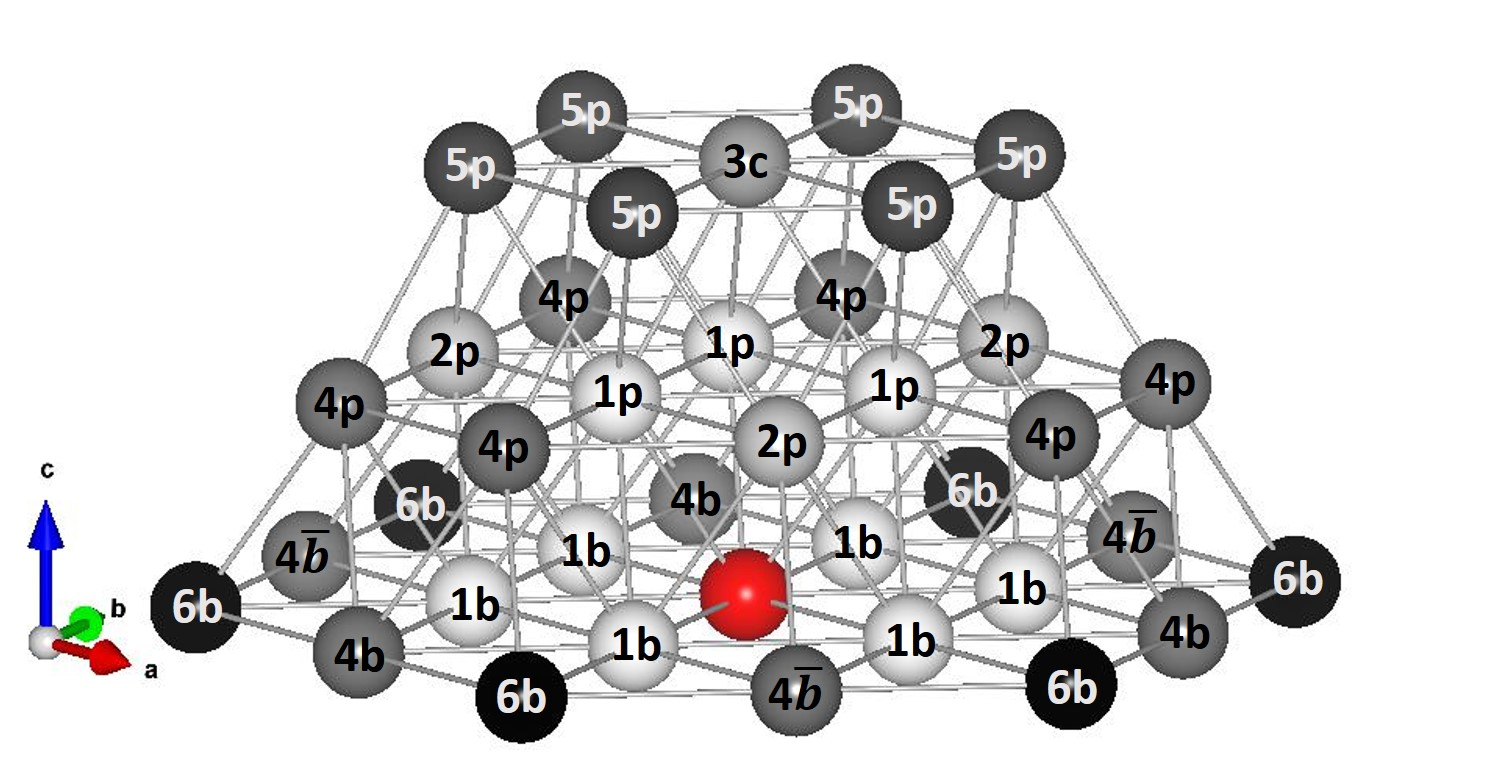
\includegraphics[width=0.8\textwidth]{configurations_labelled.jpg}
%DIFDELCMD <     %%%
\DIFdelendFL \DIFaddbeginFL 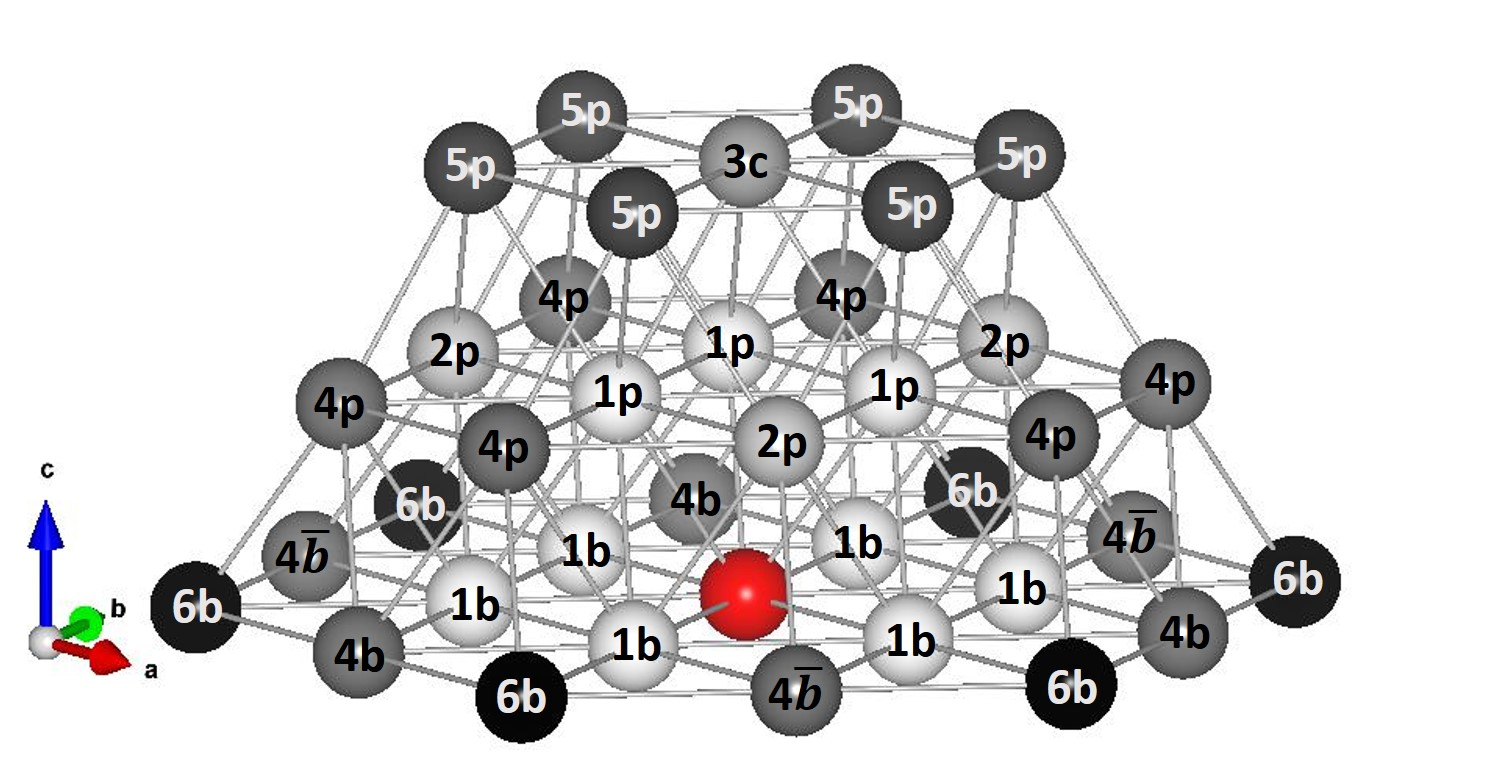
\includegraphics[width=0.8\textwidth]{1_configurations_labelled.jpg}
    \DIFaddendFL \caption{The possible vacancy-solute configurations within the $6^{th}$ nearest neighbor shell in HCP Zr. Three basal planes are shown with the solute atom (red) in the first basal plane at the bottom. The atoms with lighter colors are closer to the solute and those with darker colors have larger separation distances. The lattice sites are labeled with a number between 1 and 6 denoting the nearest neighbor number to the solute and a letter (b, p, or c) denoting the vacancy-solute orientation: basal, pyramidal, or axial (along the c-axis), respectively. \DIFaddbeginFL \DIFaddFL{The notations are inspired by those presented by Agarwal and Trinkle \cite{agarwal_exact_2017}.}\DIFaddendFL }
    \label{fig:configurations}
\end{figure}

The migration energies of these jumps $ E_m^{i\rightarrow f}$ from an initial configuration $i$ to a final configuration $f$ is calculated as follows:

\begin{equation}
\label{eq_KRA}
    E_m^{i\rightarrow f} = E_m^0 + \DIFdelbegin \DIFdel{\frac{E_{bind}^i + E_{bind}^f}{2}
}\DIFdelend \DIFaddbegin \DIFadd{\frac{E_{bind}^i - E_{bind}^f}{2}
}\DIFaddend \end{equation}

\noindent where $E_{bind}^i$ and $E_{bind}^f$ are the binding energies of the initial and final configurations, respectively. $E_m^0$ is the migration energy of a single vacancy in the pure HCP Zr. Since we neglect the binding energies beyond the thermodynamic range (i.e., beyond the $6^{th}$ nearest neighbor), \Cref{eq_KRA} simplifies to:

\begin{equation}
      E_m^{i\rightarrow f} = E_m^0 + \frac{E_{bind}^i}{2}  
\end{equation}

The vacancy-solute configurations in the HCP Zr structure considered in this work are listed in \Cref{tab:vac-solute_distance} with the separation distance and orientation of each pair. In \Cref{tab:vac-solute_distance}, there are three different configurations for $1^{st}$ nearest neighbor vacancy-solute pairs: $1p$ for a non-basal (pyramidal) pair, $1b$ for a basal pair, and $1b'$ for a basal pair where the solute exists between two half vacancies. This $1b'$-type configuration for oversized solutes has been reported for yttrium in body-centered cubic iron ($\alpha$-Fe) \cite{bocquet_migration_2017}, lanthanides in $\alpha$-Fe \cite{yang_significant_2023}, and for multiple solutes in HCP Zr \cite{jain_first-principles_2019}. The $1b$ and $1b'$ configurations have the same orientation but the prime superscript is to differentiate between the final relaxed position of the solute. In the case of $1b$, the solute atom remains on the lattice site while the solute atom falls into an intermediate position in the case of $1b'$. It should be noted that the two basal $4^{th}$ nearest neighbor configurations $4b$ and $4\overline{b}$ are symmetrically nonequivalent. They both can exist for any solute species and they have different binding energies as observed by Agarwal and Trinkle \cite{agarwal_exact_2017} in HCP \DIFdelbegin \DIFdel{magnesium }\DIFdelend \DIFaddbegin \DIFadd{Mg }\DIFaddend and by Jain et al. \cite{jain_first-principles_2019} in HCP Zr.

\begin{table}[h!]
    \centering
    \caption{Vacancy-solute configurations in HCP Zr. The letters p and b in the notations denote that the vacancy-solute pair lies within the same pyramidal or basal plane, respectively. The letter c means the vacancy-solute pair lies on the same c-axis.}
    \label{tab:vac-solute_distance}
    \begin{tabular}{c|c|c}
        \toprule
         Notation& Distance ({\AA})& Direction  \\
         \hline
         1p&3.19 & [2 4 $\overline{6}$ 3] \\
         1b&3.23 &[1 0 $\overline{1}$ 0] \\
         1b'& - & [1 0 $\overline{1}$ 0] \\
         2p&4.54 &[$\overline{4}$ $\overline{8}$ 12  3] \\
         3c&5.17 &[0 0 0 1] \\
         4p &5.57 &[2 10 $\overline{12}$ 3] \\
         4b&5.60 &[2 1 $\overline{3}$ 0] \\
         4$\overline{b}$&5.60 &[1 $\overline{1}$ 0 0] \\
         5p &6.10 & [1 0 $\overline{1}$ 1]\\
         6b &6.47 &[1 0 $\overline{1}$ 0] \\
         \bottomrule
    \end{tabular}
\end{table}

%DIF < In this subsection, 
The governing equations used to calculate point defect formation, binding, and migration energies are presented below. First, the formation energy of a single vacancy $E_{form}^{vac}$ is calculated as follows:
\begin{equation}
\label{eq_Ef_vac}
   E_{form}^{vac} = E^{vac}_{defect}[(N-1)Zr] - \frac{N-1}{N} E_{perfect}[(N) Zr] 
\end{equation}

\noindent where $E^{vac}_{defect}[(N-1)Zr]$ is the DFT energy of the defective supercell with a mono-vacancy having (N-1) Zr atoms, and $E_{perfect}[(N) Zr]$ is the DFT energy of the perfect (undefective) supercell with (N) Zr atoms. The formation energy of a substitutional defect for solute $X$, $E_{form}^{sub,X}$, is given by:
\begin{equation}
\label{eq_Ef_sub}
    E_{form}^{sub,X} = E_{defect}^{sub}[(N-1)Zr + X] - \frac{N-1}{N}E_{perfect}[(N) Zr] - E_{X}
\end{equation}
where $E_{defect}^{sub}[(N-1)Zr + X]$ is the DFT energy of the supercell with solute X as a substitutional and $E_X$ is the DFT energy per atom of element $X$ in its pure crystalline form. The formation energy of a vacancy-solute pair, $E_{form}^{sub-vac,X}$, for solute element $X$ is calculated similarly as follows:
\begin{equation}
\label{eq_Ef_vac_sub}
    E_{form}^{sub-vac,X} = E_{defect}^{sub-vac}[(N-2)Zr + X] - \frac{N-2}{N}E_{perfect}[(N) Zr] - E_{X}
\end{equation}

The vacancy-solute binding energies are calculated from the three formation energies in \Cref{eq_Ef_vac}, \Cref{eq_Ef_sub}, and \Cref{eq_Ef_vac_sub} using the following expression:
\begin{equation}
\label{eq_Eb}
    E_{bind}^{sub-vac,X} = E_{form}^{vac} + E_{form}^{sub,X} - E_{form}^{sub-vac,X}
\end{equation}
and, according to this definition, positive binding energy is attraction while negative binding energy means repulsion. These binding energies and the frequencies of each possible jump between the configurations in \Cref{tab:vac-solute_distance} are the input to the KineCluE code to calculate transport coefficients. The jump frequency, $\omega^{i\rightarrow f}$, for a transition from initial configuration (i) to final configuration (f) is: \begin{equation}
    \omega^{i\rightarrow f} = \nu^{i\rightarrow f} e^{\frac{-E_m^{i\rightarrow f}}{k_B T}}
\end{equation}
where $E_m^{i\rightarrow f}$ is the migration barrier for the jump from (i) to (f) which is calculated from the differences between the ground state energy of the initial configuration $E_i$ and the saddle point energy along the minimum energy path between the initial and final configurations, $E_s^{i\rightarrow f}$. $\nu^{i\rightarrow f}$ is the attempt frequency and is calculated from the phonon frequencies of the initial relaxed state and the transition state (saddle point) of the jump based on Vineyard's harmonic transition state theory \cite{vineyard_frequency_1957}. For computational purposes, the full Vineyard expression is approximated to consider the hopping atoms only as follows:
\begin{equation}
    \nu^{i\rightarrow f} = \frac{\Pi^{3N_{hop}}_j  \nu^{i}_j}{\Pi^{3N_{hop}-1}_j  \nu^{s,i\rightarrow f}_j}
\end{equation}
where $N_{hop}$ is the number of hopping atoms, which is 1 in most of the jumps considered and 2 in the jumps involving the 2 half-vacancies configuration. $\nu^{i}_j$ and $\nu^{s,i\rightarrow f}_j$ are phonon frequencies of the relaxed initial (i) configuration and the saddle point configuration, respectively. \DIFaddbegin \DIFadd{The approximation where only the phonon frequencies of the hopping atoms are considered significantly reduces the computing time. This should capture most of the vibrational contribution. However, the phonon frequencies of all surrounding atoms may be required to get quantitatively more accurate attempt frequencies. In the work done by Wu et al. \cite{wu_high-throughput_2016}, this approximation showed a reasonable accuracy and introduced an error by a factor of 2-2.5 in FCC and HCP systems. }\DIFaddend Finally, the vacancy formation entropy, $S_{form}^{vac}$, was calculated from the vibrational frequencies of the perfect, $\nu_j^{perfect}$, and defective supercells, $\nu_j^{def}$, as follows:
\begin{equation}
    S_{form}^{vac} = k_B ln(\frac{\Pi^{3N-1}_j \nu_j^{perfect}}{\Pi^{3N-1}_j \nu_j^{def}})
\end{equation}
where N is the total number of atoms in the perfect supercell. To reduce the computational expense, we obtained the vibrational frequencies of only the 12 Zr atoms which are the $1^{st}$ nearest neighbors to the vacancy atom. This $1^{st}$ nearest neighbor shell has the highest strain and is expected to have the highest contribution to $S_{form}^{vac}$. \DIFaddbegin \DIFadd{Similar to the approximation used in calculating the attempt frequencies, the approximation used for the vacancy formation entropy is expected to introduce a minor error that will not impact any qualitative conclusions in this work.
}\DIFaddend 

\FloatBarrier

\subsection{Density Functional Theory Computational Details}

DFT calculations were performed using the projector-augmented wave method \cite{blochl_projector_1994} as implemented in the VASP software \cite{kresse_ab_1993, kresse_efficient_1996}. All calculations were performed using a non-spin-polarized setting. The Perdew-Burke-Ernzerhof generalized gradient approximation \cite{perdew_generalized_1996} was utilized as the exchange-correlation functional. A plane-wave cutoff energy of 450 eV was applied in all calculations. $5\times5\times3$ supercells (150 atoms) were adopted in point defect energy calculations. The Brillouin zone sampling for these supercells was done using a $4\times4\times4$ $\Gamma$-centered k-points mesh. The Methfessel-Paxton smearing method was used with a width of 0.1 eV  \cite{methfessel_high-precision_1989}. The geometry relaxation of supercells with point defects was performed under a fixed volume constraint with a force convergence criterion of 5 meV/{\AA} using the conjugate gradient algorithm. The migration barriers of vacancy jumps were calculated using the \DIFdelbegin \DIFdel{climbing-image }\DIFdelend \DIFaddbegin \DIFadd{climbing image }\DIFaddend nudged elastic band (CI-NEB) method \cite{henkelman_climbing_2000} with a single intermediate image. 3-image CI-NEB was tested for the monovacancy jumps and the vacancy-solute jumps that start from the 2 half-vacancies, and produced the same results. Finally, the phonon calculations were performed by calculating the force constants using the finite-differences approach as implemented in VASP \cite{kresse_ab_1993,kresse_efficient_1996}. Displacements of width 0.02 {\AA} were applied to atoms to calculate the Hessian matrix \cite{hafner_ab-initio_2008}.

\FloatBarrier

\section{Results}
\label{results}

\subsection{Lanthanide-Vacancy Interactions and Migration}
\DIFaddbegin \label{lanthanide_vac_inter}
\DIFaddend 

The calculated value for vacancy formation energy $E_{form}^{vac}$ is 2.007 eV\DIFaddbegin \DIFadd{, }\DIFaddend which is in reasonable agreement with the DFT values in the literature: 2.002 \cite{jain_first-principles_2019}, 2.01 \cite{lu_first-principles_2018}, 2.07 \cite{varvenne_vacancy_2014}, and 1.95 \cite{pasianot_issues_2012} eV. The vacancy formation entropy $S_{form}^{vac}$ was found to be 1.122 $k_B$. The only calculation of $S_{form}^{vac}$ in HCP Zr in the literature was done by Pasianot and P\'erez \cite{pasianot_issues_2012}. They reported two values of 1.51 and 3.69 $k_B$ from 36-atoms and 96-atoms supercells, respectively. They also suggested a corrective -10\% for the 3.69 $k_B$ value to be 3.19 $k_B$. Since the vacancy concentration $[V]$ varies exponentially with $S_{form}^{vac}$ as seen in \Cref{eq_vac_conc}, the difference between using our value 1.122 $k_B$ and their value 3.19 $k_B$ \cite{pasianot_issues_2012} will result in a factor of 8 difference in the calculated diffusivities. However, it will not affect other quantities such as normalized transport coefficients, vacancy drag ratios, or any ratios between transport coefficients. 

The binding energies for all the considered lanthanide-vacancy pairs are given in \Cref{tab:BE}. All species exhibit an attractive binding for a 1$^{st}$ nearest neighbor pair, but \DIFdelbegin \DIFdel{we observe }\DIFdelend a relatively stronger attractive binding \DIFaddbegin \DIFadd{is observed }\DIFaddend for the La-vacancy pair in both the basal and pyramidal configurations compared to the other fission product species investigated. 
On the other hand, Pr is observed to have the weakest attractive binding with vacancies among the four lanthanides. The binding energies generally decrease with distance and no lanthanide-vacancy pair has an interaction larger than 0.05 eV beyond the 3$^{rd}$ nearest neighbor. 

\begin{table}[h!]
    \centering
    \caption{Binding energies in eV for lanthanide-vacancy pairs. Positive binding energies are attractive and negative binding energies are repulsive.}
    \label{tab:BE}
    \begin{tabular}{c|c|c|c|c}
        \toprule
       Configuration & La-vacancy & Ce-vacancy & Pr-vacancy & Nd-vacancy  \\
       \hline
       1p &0.389 &0.182 &0.103 &0.261 \\
       1b &- &- &- &0.226 \\
       1b' &0.358 &0.230 &0.151 &- \\
       2p &-0.081 &-0.050 &-0.056 &-0.077 \\
       3c &0.015 &0.085 &0.070 &-0.025 \\
       4p &-0.012 &-0.016 &-0.024 &-0.008 \\
       4b &-0.001 &0.010 &0.014 &-0.004 \\
       4$\overline{b}$ &0.015 &-0.014 &-0.043 &0.022 \\
       5p &-0.007 &-0.006 &-0.021 &-0.012 \\
       6b &-0.003 &-0.015 &-0.035 &0.003 \\
       \bottomrule
    \end{tabular}
\end{table}

The migration barriers and attempt frequencies of mono-vacancy jumps in pure Zr and solute-vacancy exchange jumps are shown in \Cref{tab:jumps}. 
\DIFdelbegin \DIFdel{It should }\DIFdelend \DIFaddbegin \DIFadd{The low migration barriers for the pyramidal solute-vacancy exchange of La and Ce are comparable to the value of $k_B$$T$, particularly at high temperatures. This raises questions about the validity of the transition state theory in this context. However, the calculation of solute transport coefficients also depends on other migration barriers, with the complete list shown in Tables \ref{tab:jumps_vac_oversized} and \ref{tab:jumps_vac_nd}. Therefore, even if these jumps are nearly instantaneous, they do not serve as the rate-limiting step in the diffusion behavior of these solutes.
It should also }\DIFaddend be noted that the basal solute-vacancy exchange jump is only allowed for Nd (\Cref{fig:basal_jumps_1b_and_1bb}(a)) and is not allowed for the oversized solutes, La, Ce, and Pr. In the case of the 1b configuration in \Cref{fig:basal_jumps_1b_and_1bb}(a), the vacancy-solute exchange jump is allowed (black arrow) and the colored arrows represent other possible jumps 1b-1b, 1b-4b, 1b-4$\overline{b}$, and 1b-6b, where the Ln atom remains on the lattice site. In the case of oversized solutes in \Cref{fig:basal_jumps_1b_and_1bb}(b), the vacancy-solute exchange is not allowed. In the 1b'-1b' jump, one of the first nearest neighbor atoms migrate to one of the two half vacancies and the solute atom moves to occupy the intermediate position (dashed circle) between the newly-formed two half vacancies. In the 1b'-4b, 1b-4$\overline{b}$, and 1b-6b jumps, the solute moves back to the lattice site, and the atom on the 4b, 4$\overline{b}$, or 6b site moves to one of the two half vacancies. The possible pyramidal jumps from the 1b configuration for Ln and the oversized solutes are shown in \Cref{fig:pyr_jumps_1b_and_1bb}. \DIFaddbegin \DIFadd{Both \Cref{fig:basal_jumps_1b_and_1bb}(a) and \Cref{fig:pyr_jumps_1b_and_1bb}(a) are inspired by the paper by Agarwal and Trinkle \cite{agarwal_exact_2017} on HCP Mg. Herein it is modified to visualize the jump starting from the two half vacancies configuration (1b') in \Cref{fig:basal_jumps_1b_and_1bb}(b) and \Cref{fig:pyr_jumps_1b_and_1bb}(b) for oversized solutes in HCP Zr.
}\DIFaddend 

\begin{table}[h!]
    \centering
    \caption{The migration energies and attempt frequencies of Zr single vacancy jumps and solute-vacancy exchange jumps.}
    \begin{tabular}{c|c|c|c}
    \toprule
        Solute & Jump & $E_m$ (eV) & $\nu$ (THz) \\
        \hline
       -  &basal&0.567 & 4.65\\
       - &pyramidal &0.649 & 4.58\\
       \hline
       La&pyramidal &0.049 &1.81 \\
       Ce&pyramidal &0.090 &2.16 \\
       Pr&pyramidal &0.158 &2.85 \\
       Nd&basal &0.117 &2.62 \\
       Nd&pyramidal &0.140 &2.26 \\
       \bottomrule
    \end{tabular}
    \label{tab:jumps}
\end{table}

\begin{figure}[h!]
    \centering
    \DIFdelbeginFL %DIFDELCMD < 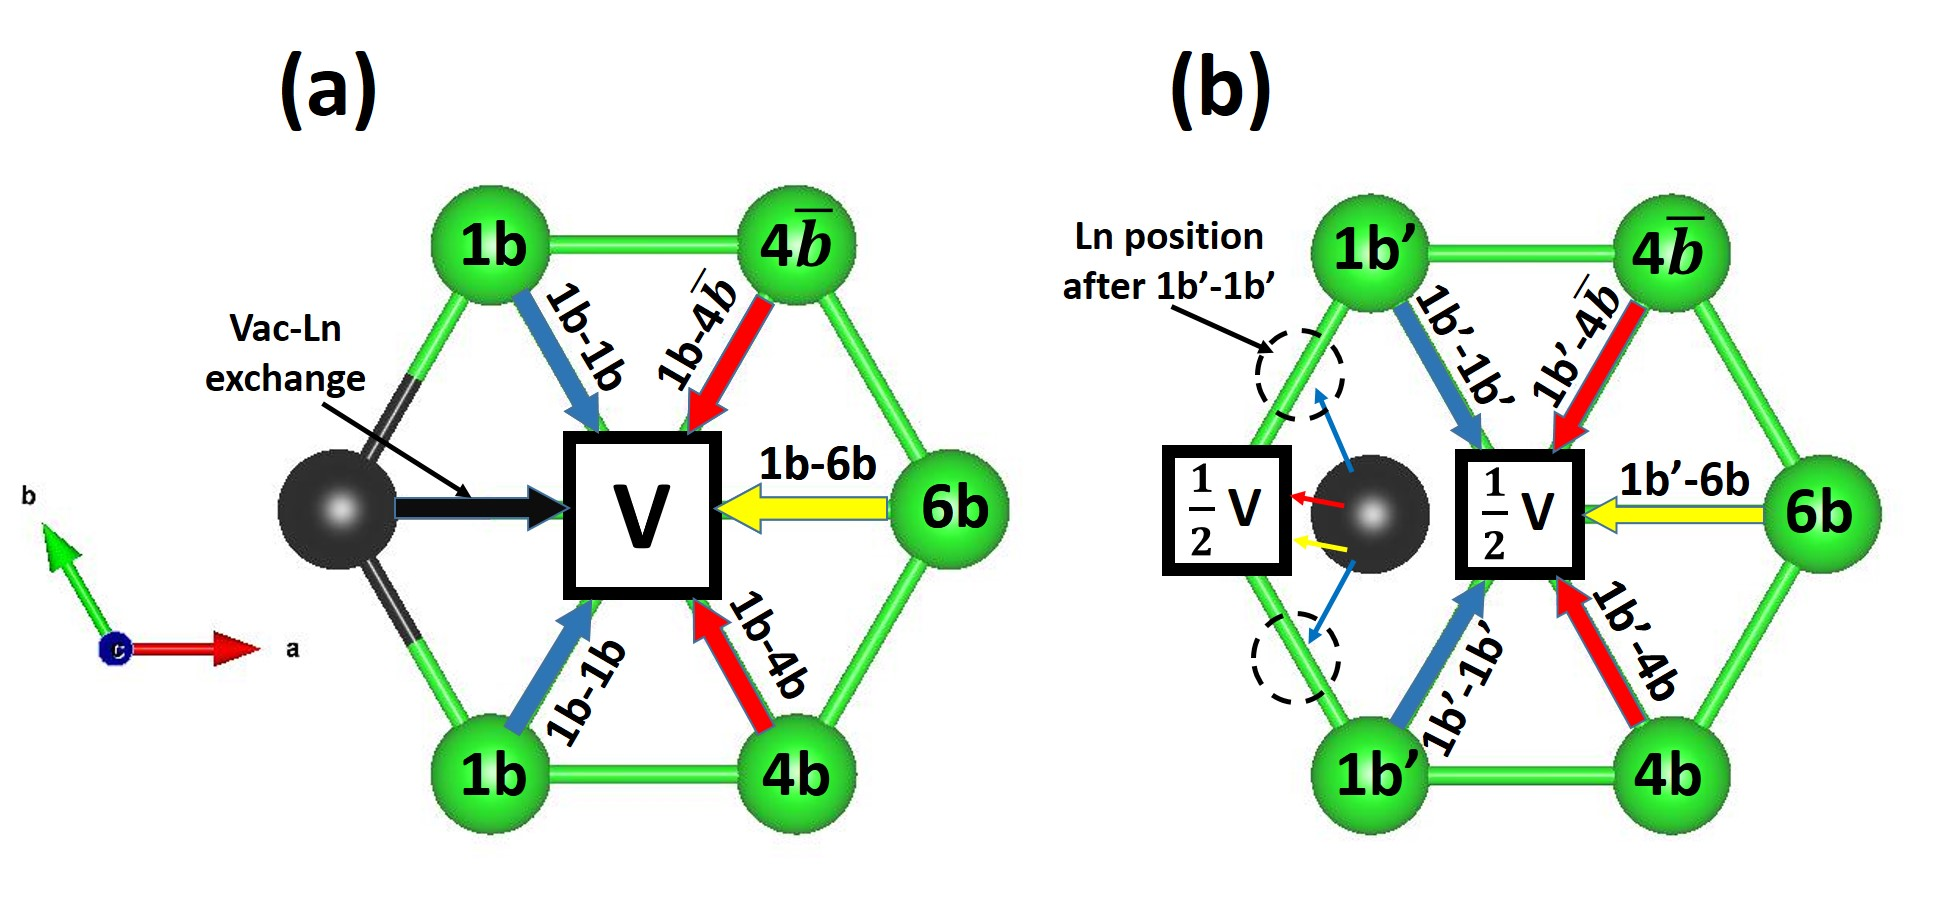
\includegraphics[scale=0.5]{basal_jumps_1b_1bb.jpg}
%DIFDELCMD <     %%%
\DIFdelendFL \DIFaddbeginFL 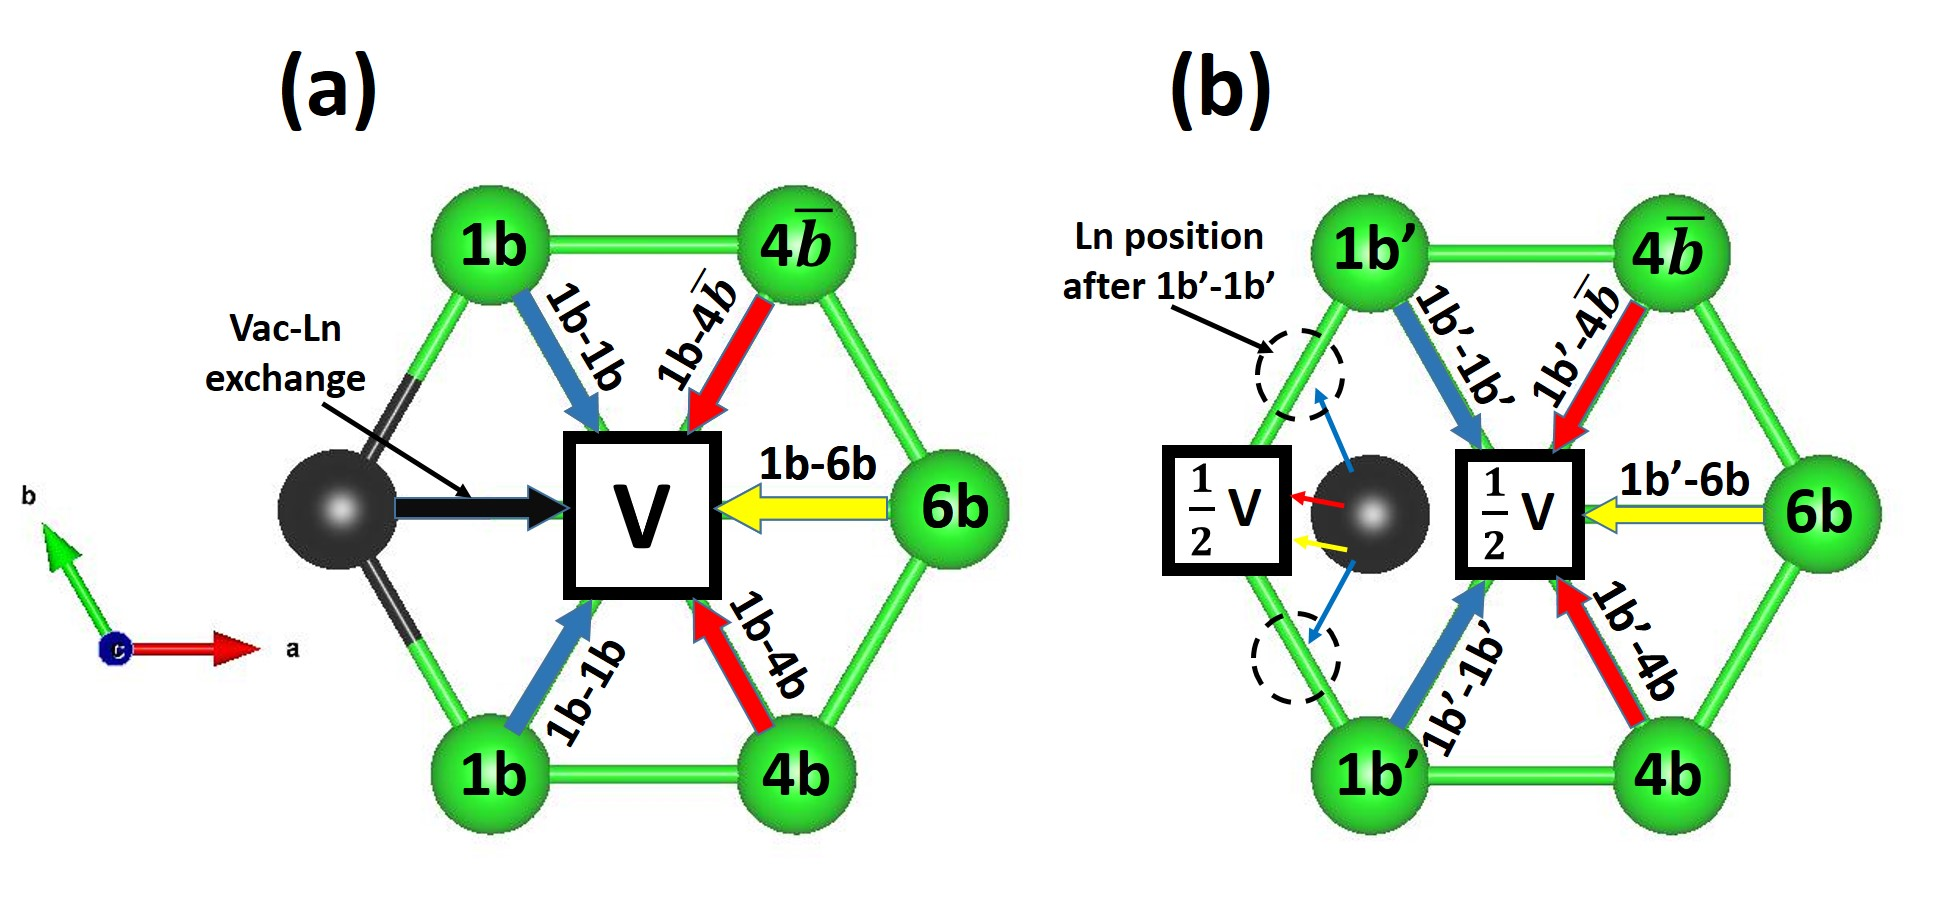
\includegraphics[width=0.9\textwidth]{2_basal_jumps_1b_1bb.jpg}
    \DIFaddendFL \caption{Possible basal jumps starting from the 1b configuration in panel (a) which applies for the Nd solute, and from the 1b' configuration in panel (b) which applies for La, Ce, and Pr. The lanthanide solute atom (Ln) is shown as a black sphere while Zr host atoms are green spheres. The vacancy and half vacancies are represented by empty squares. }
    \label{fig:basal_jumps_1b_and_1bb}
\end{figure}

\begin{figure}[h!]
    \centering
    \DIFdelbeginFL %DIFDELCMD < 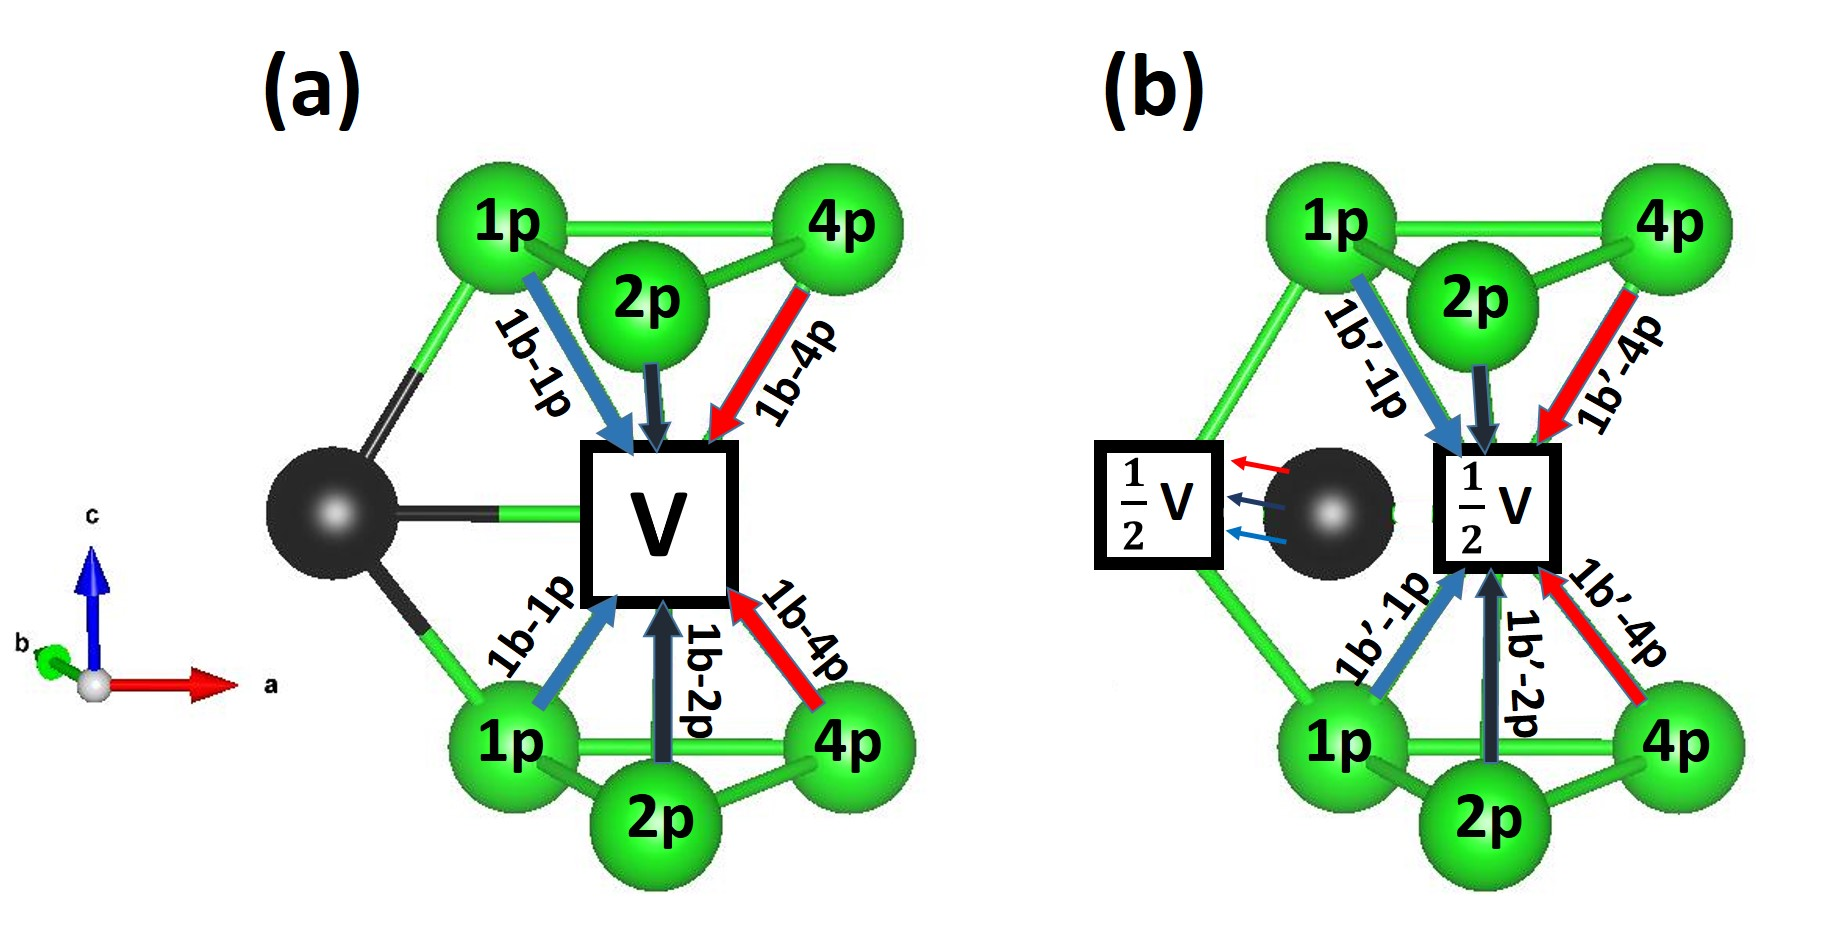
\includegraphics[scale=0.5]{pyramidal_jumps_1b_1bb.jpg}
%DIFDELCMD <     %%%
\DIFdelendFL \DIFaddbeginFL 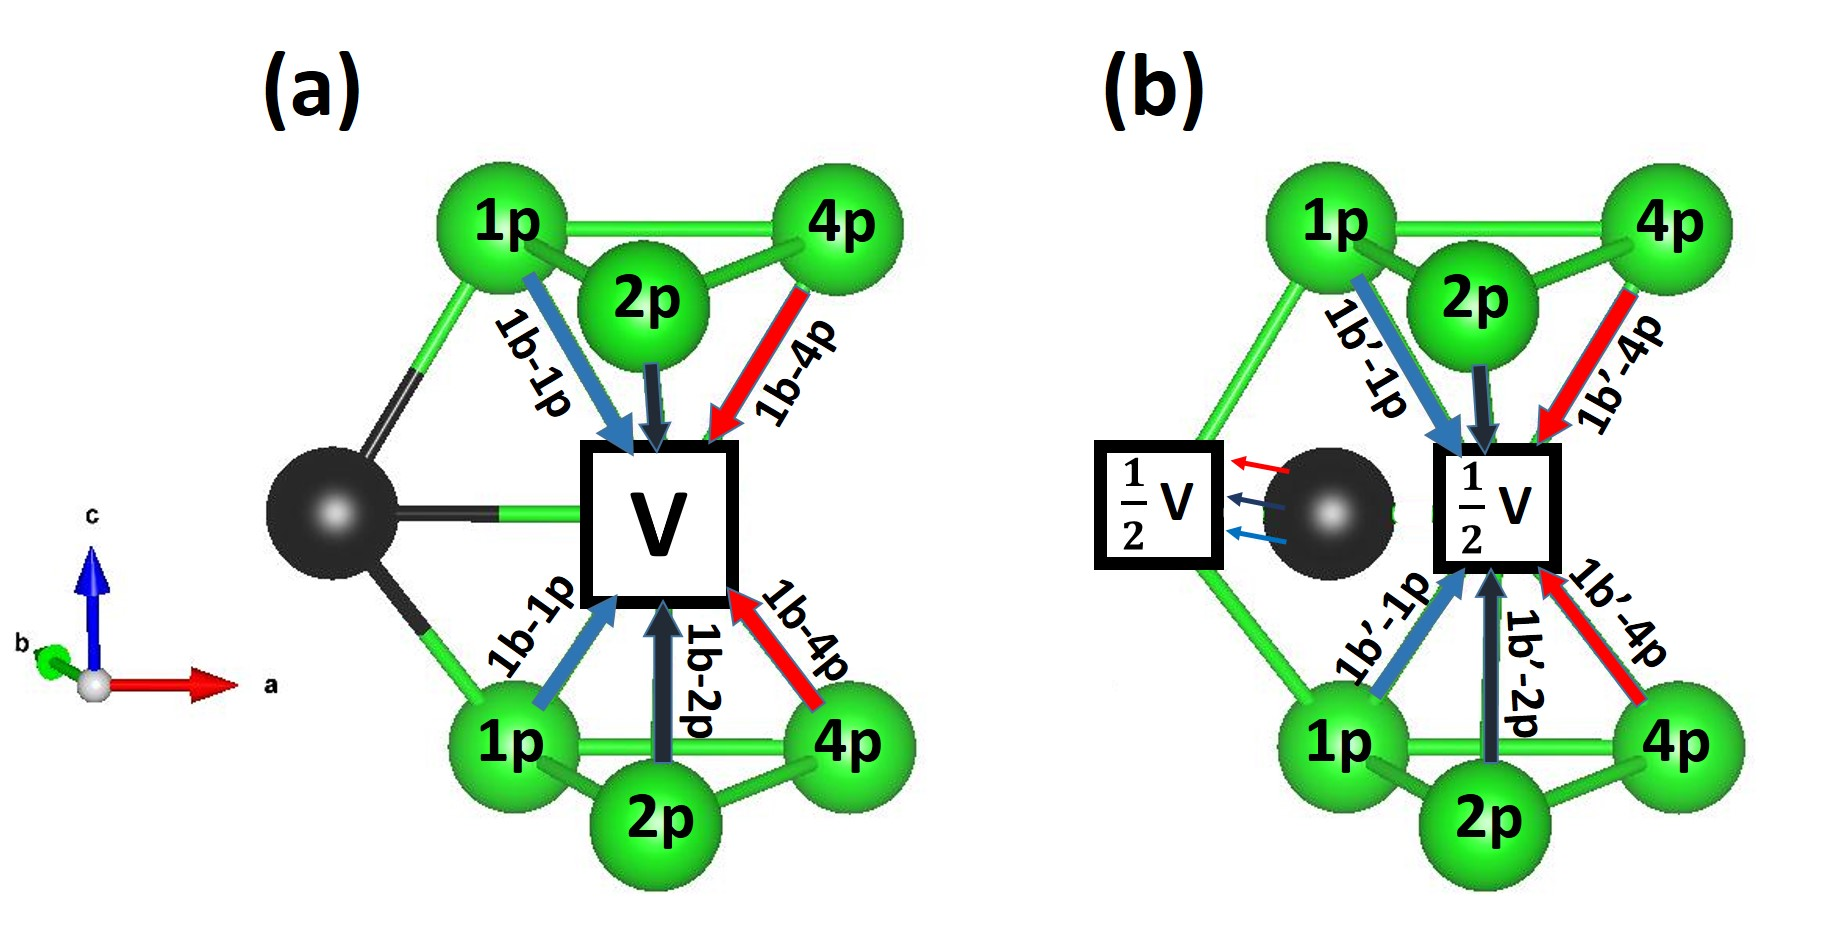
\includegraphics[width=0.9\textwidth]{3_pyramidal_jumps_1b_1bb.jpg}
    \DIFaddendFL \caption{Possible pyramidal jumps starting from the 1b configuration in panel (a) for Nd in HCP Zr and from the 1b' configuration in panel (b) for La, Ce, or Pr in HCP Zr.The lanthanide solute atom (Ln) is shown as a black sphere while Zr host atoms are green spheres. The vacancy and half vacancies are represented by empty squares.}
    \label{fig:pyr_jumps_1b_and_1bb}
\end{figure}

The migration energies of the basal and pyramidal mono-vacancy jumps in pure HCP Zr are 0.567 eV and 0.649 eV, respectively. These values are consistent with DFT calculations in the literature: 0.51 \cite{verite_anisotropy_2007}, 0.538 \cite{samolyuk_analysis_2014}, and 0.553 \cite{jain_first-principles_2019} eV for the basal jump, and  0.67 \cite{verite_anisotropy_2007}, 0.629 \cite{samolyuk_analysis_2014}, and 0.613 \cite{jain_first-principles_2019} eV for the pyramidal jump. However, we do not observe the double-humped barrier for the basal vacancy jump that is reported by Samolyuk et al. \cite{samolyuk_analysis_2014} and Jain et al. \cite{jain_first-principles_2019}. The migration barriers presented in \Cref{tab:jumps} were obtained using 1-image and 3-image CI-NEB and the corresponding attempt frequencies were calculated using the same supercell size. Both 1-image and 3-image CI-NEB calculations yielded the same barrier shape and migration energy values within a 0.01 eV difference. The double-humped barrier reported in the literature may be a finite-size artifact. In this work, all calculations were performed using the $5\times5\times3$ supercell while the $4\times4\times3$ supercell was used in the prior references \cite{samolyuk_analysis_2014, jain_first-principles_2019} which used VASP \cite{kresse_ab_1993} and QuantumESPRESSO \cite{giannozzi_quantum_2009}, respectively. Jain et al.~tested the $6\times6\times4$ supercell \cite{jain_first-principles_2019} in another DFT code, CASTEP \cite{clark_first_2005}. \DIFdelbegin \DIFdel{They }\DIFdelend \DIFaddbegin \DIFadd{Jain et al. \cite{jain_first-principles_2019} }\DIFaddend emphasize that metastable states exist for substitutional solute jumps in the basal plane regardless of the supercell size. When we tested the $4\times4\times3$ supercell, we also did not observe that double-humped barrier.

The full set of migration barriers and attempt frequencies of vacancy jumps in lanthanide-containing Zr are listed in \ref{app:dft_data} in \Cref{tab:jumps_vac_oversized} and \Cref{tab:jumps_vac_nd} for oversized substitutional systems (Zr-La, Zr-Ce, and Zr-Pr), and Zr-Nd, respectively. In both tables, there are 23 possible vacancy jumps within the $6^{th}$ nearest neighbor distance. The majority of these jumps are direct transitions between the lattice sites shown in \Cref{fig:configurations}. However, for the case of oversized substitutionals (La, Ce, and Pr), the $1^{st}$ nearest neighbor Ln-vacancy pairs in the basal plane have the 1b' configuration instead of the regular 1b configuration observed for \DIFaddbegin \DIFadd{the }\DIFaddend Nd-vacancy pair. The 1b' configuration denotes the two-half-vacancies configuration in the basal plane.


The attempt frequencies for the basal jumps 1b'-1b' and the pyramidal jumps 1b'-1p were calculated for each lanthanide species. For computational purposes, we assumed the attempt frequency of any basal jump starting from 1b' is equal to that of 1b'-1b'. Similarly, we assume that the attempt frequency of any pyramidal jump starting from 1b' is equal to that of 1b'-1p. Other basal and pyramidal jumps starting from different configurations (not 1b') are assumed to have the same attempt frequency as the monovacancy basal and pyramidal jumps, respectively. The calculated attempt frequencies for monovacancy jumps in pure HCP Zr are 4.65 THz and 4.58 THz, for the basal and pyramidal jump, respectively. Employing these values for vacancy jumps in lanthanide-containing HCP-Zr is a reasonable approximation as these jumps (all jumps except those starting from 1b' configuration) do not involve the movement of the solute atom. The same applies to all the vacancy jumps in the Zr-Nd system in \Cref{tab:jumps_vac_nd} where we also assume an attempt frequency of 4.65 THz and 4.58 THz for all basal and pyramidal jumps, respectively. Finally, all the DFT energetics and attempt frequencies presented in this subsection are used as input to the KineCluE code\cite{schuler_kineclue_2020} to calculate the transport coefficients.

\FloatBarrier

\subsection{Lanthanide Diffusivities}
\label{subsection_diffusivities}

The lanthanide diffusivities ($D_B$) are calculated from the $L_{BB}$ transport coefficient:
\begin{equation}
\DIFaddbegin \label{solute_diffusion_coeff}
    \DIFaddend D_B = \DIFdelbegin \DIFdel{\frac{L_{BB}}{[B]}
}\DIFdelend \DIFaddbegin \DIFadd{\frac{L_{BB}}{C_B}
}\DIFaddend \end{equation}
where \DIFdelbegin \DIFdel{$[B]$ is the }\DIFdelend \DIFaddbegin \DIFadd{$C_B$ is the nominal }\DIFaddend solute concentration within the dilute limit (See \ref{appendix_partition}). 
\DIFdelbegin \DIFdel{Similarly, the }\DIFdelend \DIFaddbegin 

\DIFadd{The }\DIFaddend self-diffusivity ($D_{self}$) of Zr \DIFaddbegin \DIFadd{via a vacancy mechanism }\DIFaddend can be calculated from the \DIFdelbegin \DIFdel{$L_{AA}$ transport coefficient :
}\begin{displaymath}
    \DIFdel{D_{self} = D_A = \frac{L_{AA}}{1-[B]}
\label{eq_self_diff}
}\end{displaymath}%DIFAUXCMD
\DIFdel{In }\DIFdelend \DIFaddbegin \DIFadd{$L_{VV}^{(V)}$ transport coefficient in the }\DIFaddend pure HCP Zr \DIFdelbegin \DIFdel{and at very low lanthanide concentrations, \Cref{eq_self_diff} converges to:
}\DIFdelend \DIFaddbegin \DIFadd{system (solute-free):
}\DIFaddend \begin{equation}
    D_{self} = \DIFdelbegin \DIFdel{L_{AA} = L_{VV} = }\DIFdelend \DIFaddbegin \DIFadd{f_0 }\DIFaddend C_V L_{VV}^{(V)}
\end{equation}
\DIFaddbegin \DIFadd{where $C_V$ is the equilibrium concentration of vacancies calculated by Equation \ref{eq_vac_conc} in \ref{appendix_partition}. The correlation factor for self-diffusion is $f_0$ \cite{allnatt_atomic_2003}. The value of $f_0$ can be calculated using the KineCluE code
\cite{schuler_kineclue_2020} by adding a solute species that has the same energetics as the matrix host atoms (i.e., a tracer atom).
}\DIFaddend 

The self-diffusion coefficient is plotted versus inverse temperature in \Cref{fig:self_diff}. The calculated diffusion coefficients show a reasonable agreement with experiments \cite{hood_self-_1997, horvath_anomalous_1984}. The activation energy for self-diffusion in HCP-Zr is \DIFdelbegin \DIFdel{2.572 eV and 2.649 }\DIFdelend \DIFaddbegin \DIFadd{2.579 eV and 2.644 }\DIFaddend eV in the basal and axial directions, respectively. The diffusion in the basal plane is faster than that in the axial direction at all temperatures\DIFaddbegin \DIFadd{, }\DIFaddend in agreement with the experimental measurements reported by Hood et al. \cite{hood_self-_1997}. \DIFaddbegin \DIFadd{The activation energies are also in excellent agreement with theoretical DFT studies in the literature. Lu et al. \cite{lu_first-principles_2018} reported activation energies of 2.58 eV (basal) and 2.65 eV (axial). The calculated activation energies by Pasianot and Perez \cite{pasianot_issues_2012} are 2.62 eV (basal) and 2.66 eV (axial). The discrepancy in the absolute values of self-diffusion coefficients between this work and the other DFT studies \cite{pasianot_issues_2012, lu_first-principles_2018} can be attributed to the different prefactors used in each study and in particular, $S_{form}^{vac}$, and $\nu$. Both studies \cite{pasianot_issues_2012, lu_first-principles_2018} used a value of 3.19 $k_B$ for $S_{form}^{vac}$, which was calculated by Pasianot and Perez \cite{pasianot_issues_2012}, while a value of 1.122 $k_B$ is used in this work. This leads to a factor of eight difference as mentioned earlier in section \ref{lanthanide_vac_inter}. Another difference is that in reference \cite{pasianot_issues_2012}, a relatively high value for $\nu$ (18.56 THz) was employed. The values used in this work are 4.65 and 4.58 THz, for basal and pyramidal jumps, respectively, which are in closer agreement with other DFT calculations in the literature, such as 5.205 and 5.849 THz reported by Jain et al.\cite{jain_first-principles_2019}. This difference in prefactor calculations explains the shift between the self-diffusivity calculated in this work and in other DFT studies \cite{pasianot_issues_2012, lu_first-principles_2018}.
}\DIFaddend 

\begin{figure}[h!]
    \centering
    \DIFdelbeginFL %DIFDELCMD < 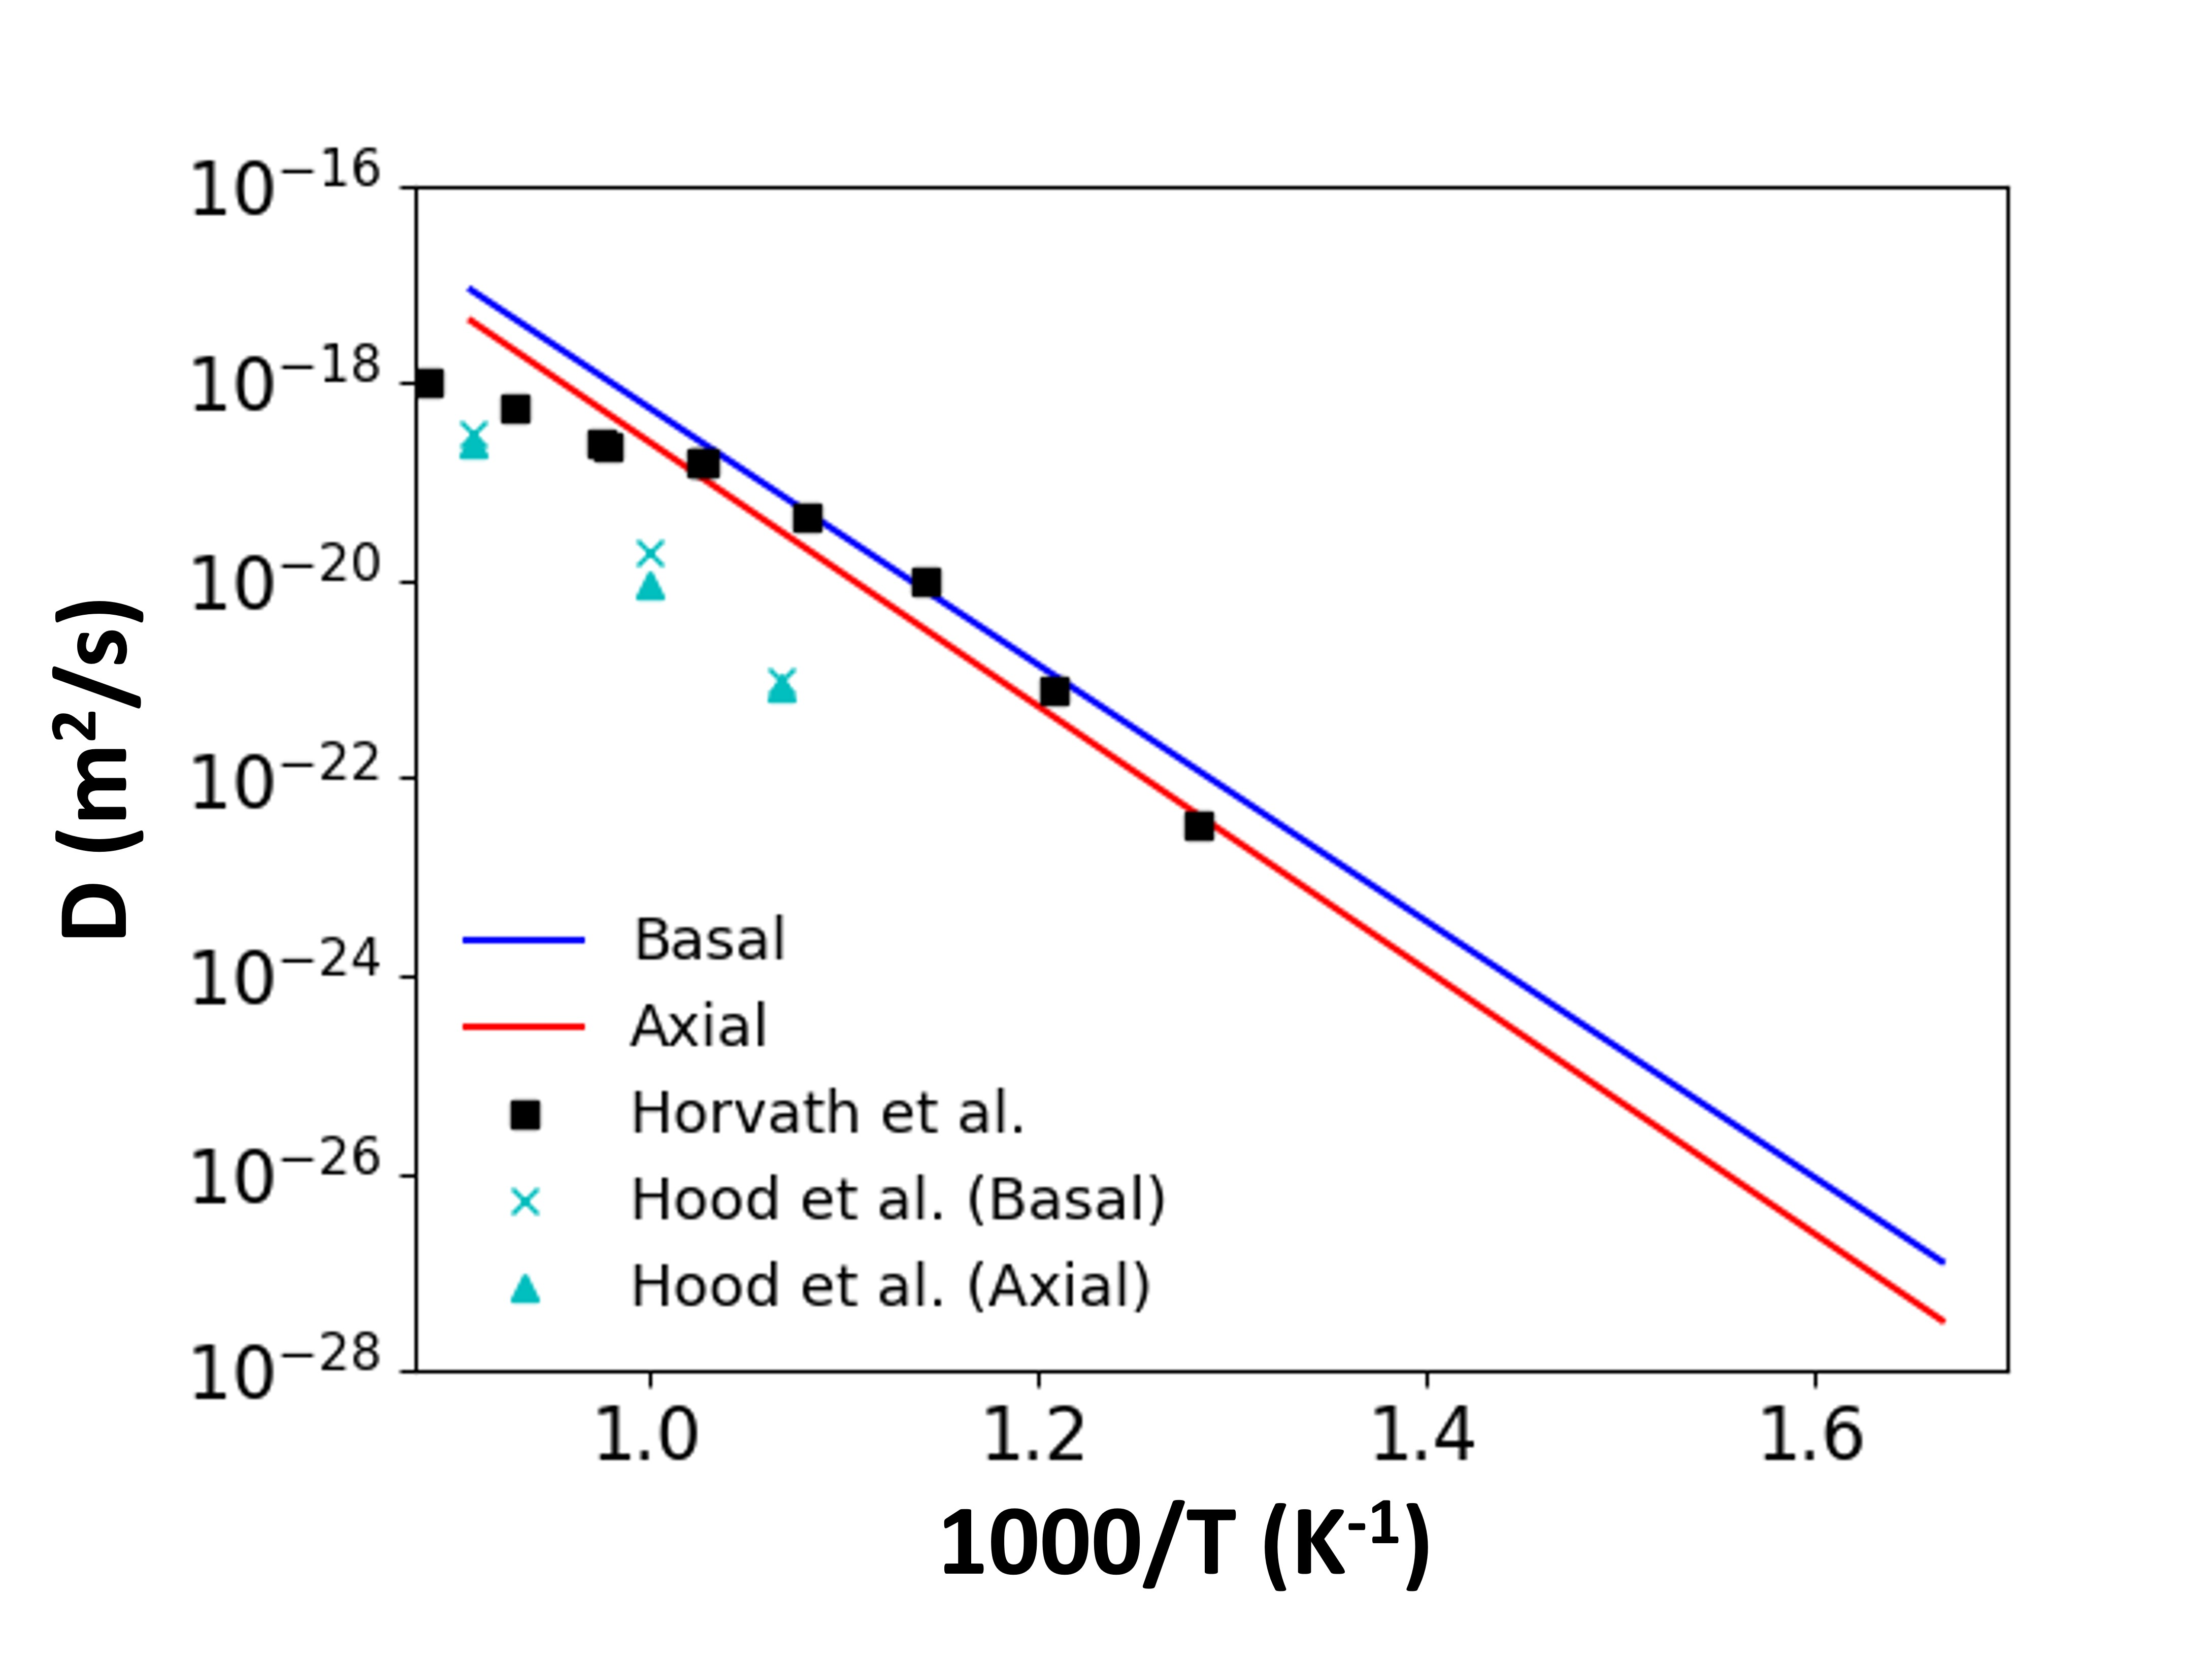
\includegraphics[width=0.8\textwidth]{self_diff_updated.jpg}
%DIFDELCMD <     %%%
\DIFdelendFL \DIFaddbeginFL 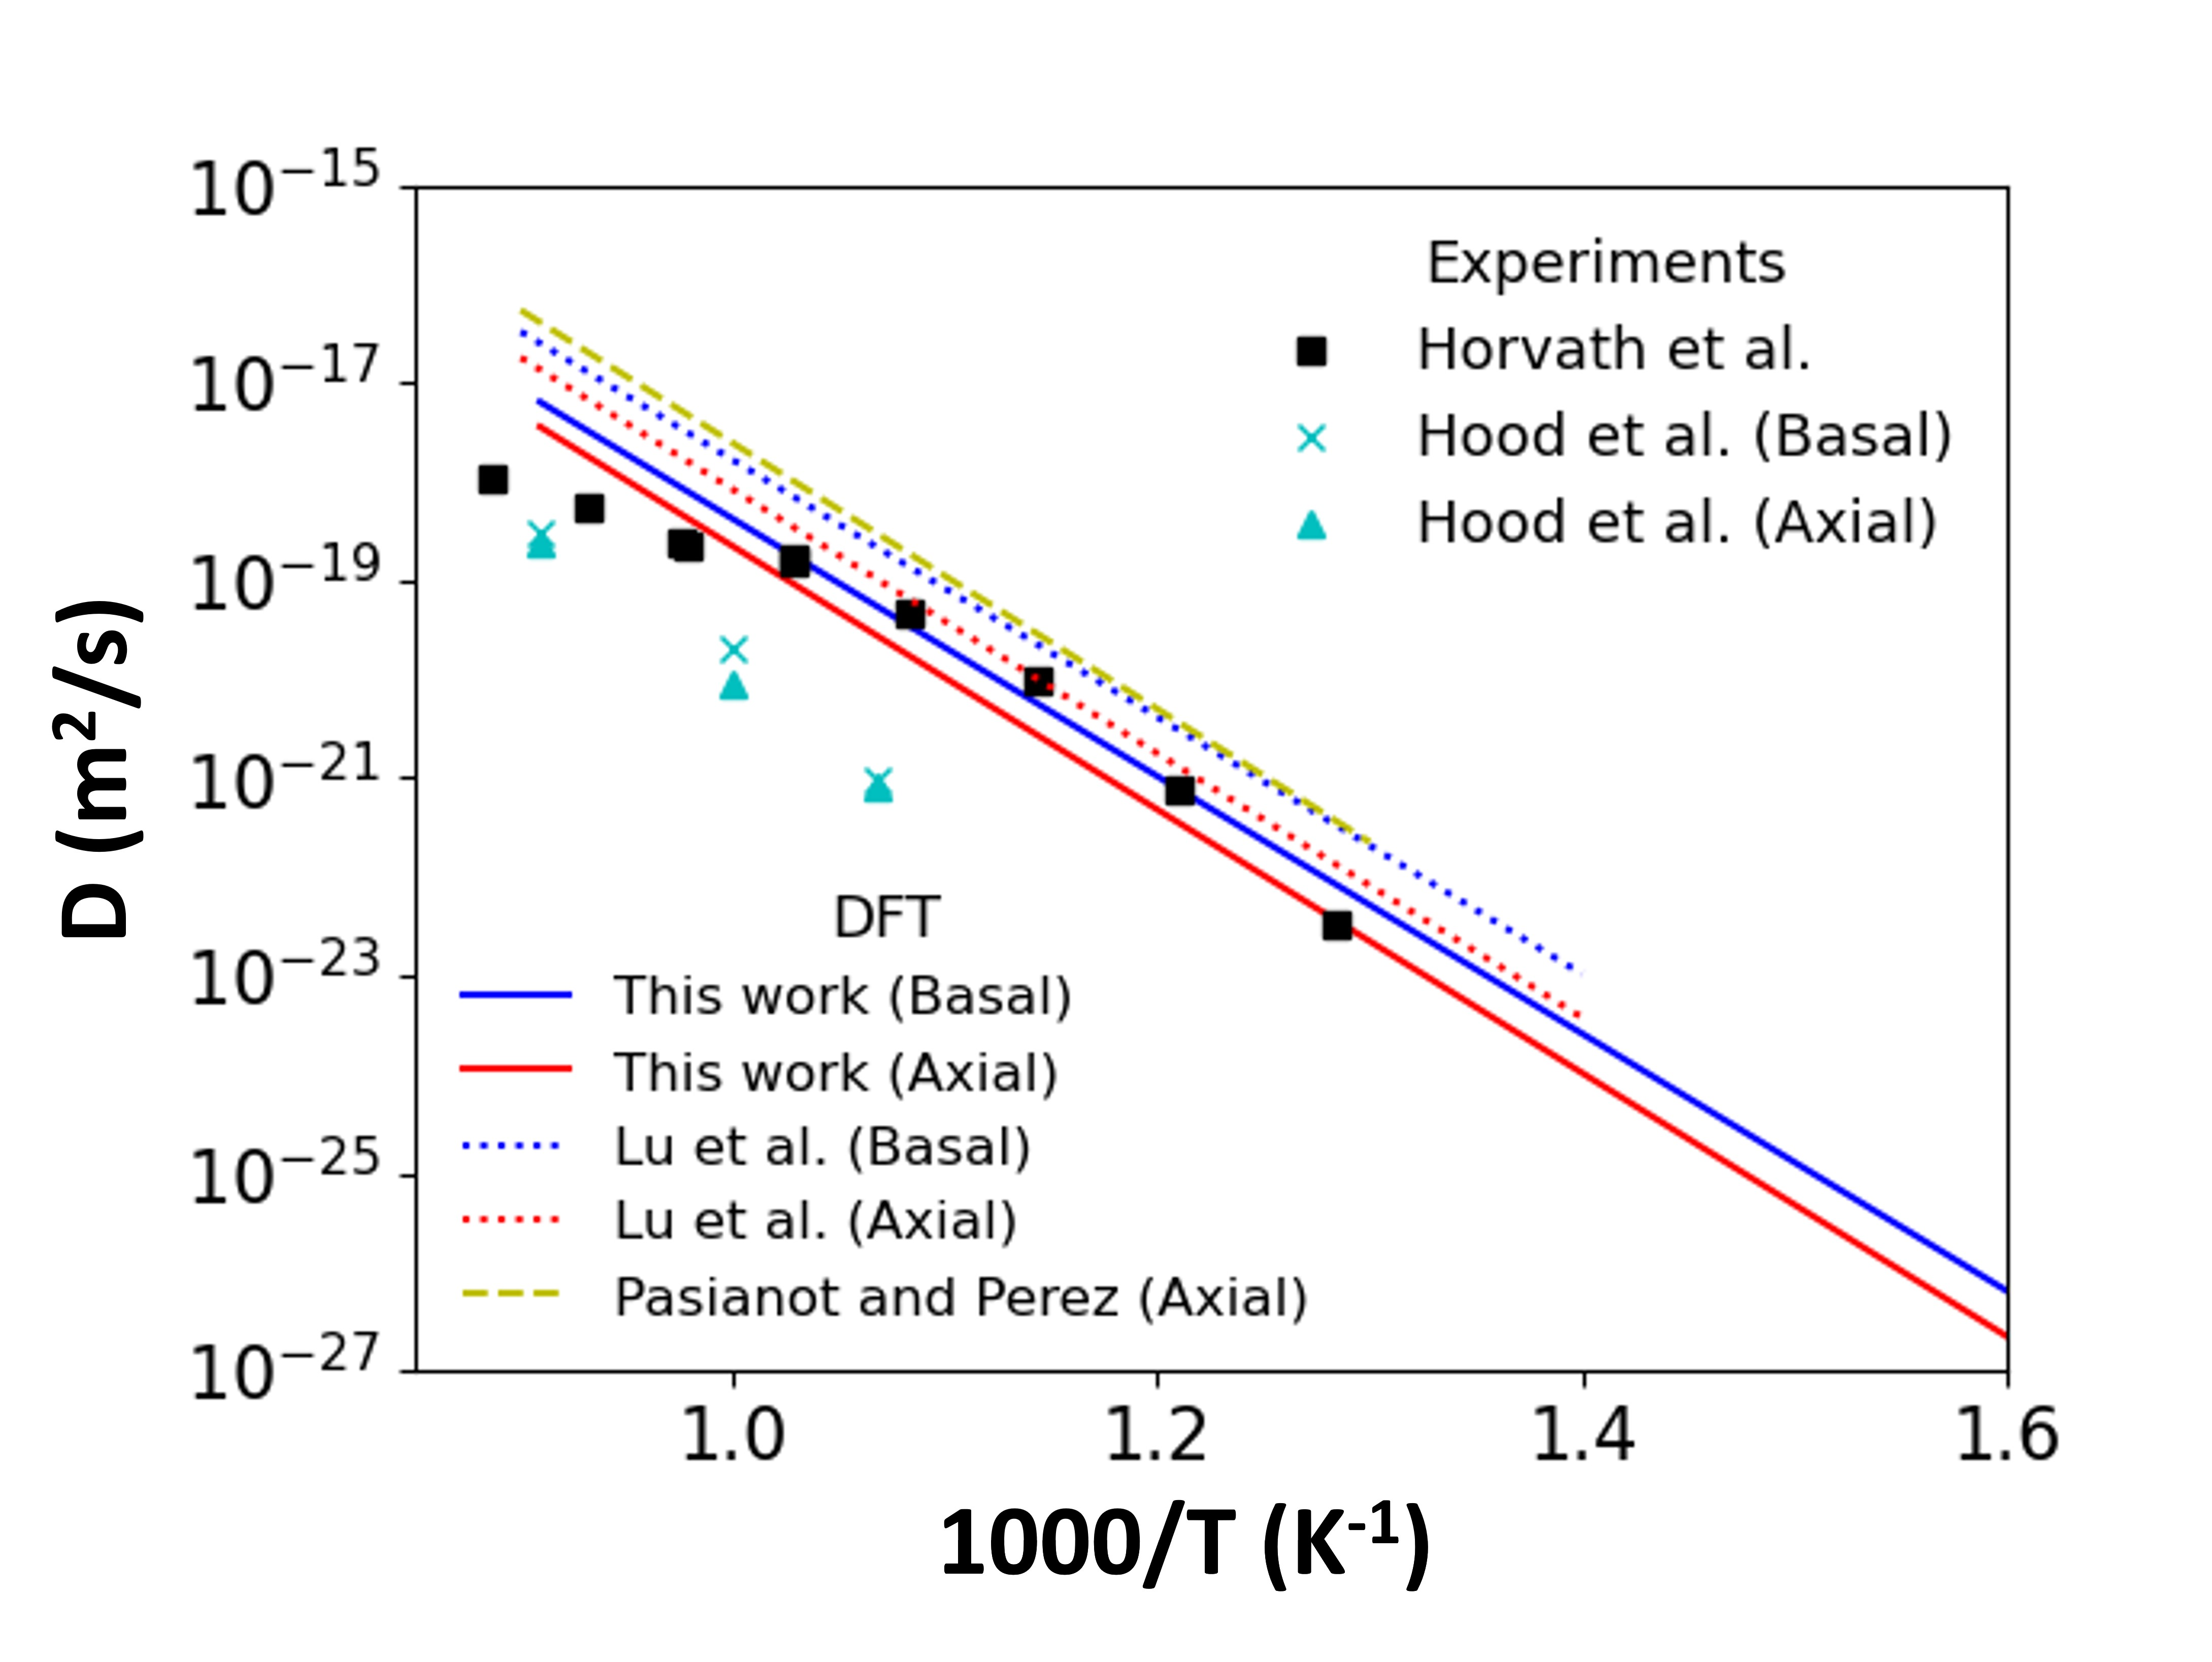
\includegraphics[width=0.7\textwidth]{4_self_diff_added_f0_dft_literature.jpg}
    \DIFaddendFL \caption{Self-diffusivity in HCP Zr via vacancy-mediated transport is plotted versus inverse temperature along basal (blue) and axial (red) directions. \DIFdelbeginFL \DIFdelFL{Scattered data }\DIFdelendFL \DIFaddbeginFL \DIFaddFL{The dotted and dashed lines are DFT-calculated self-diffusivities from references \cite{pasianot_issues_2012, lu_first-principles_2018}. Data }\DIFaddendFL points are experimental self-diffusivities from \DIFdelbeginFL \DIFdelFL{references \cite{hood_self-_1997, horvath_anomalous_1984}}\DIFdelendFL \DIFaddbeginFL \DIFaddFL{Hood et al}\DIFaddendFL . \DIFaddbeginFL \DIFaddFL{\cite{hood_self-_1997} and Horvath et al. \cite{horvath_anomalous_1984}.}\DIFaddendFL }
    \label{fig:self_diff}
\end{figure}

The diffusion coefficients of the lanthanides in Zr are plotted in \Cref{fig:diffusivities_ln} where Zr self-diffusivities are also plotted for comparison.  The diffusion coefficients were calculated from T = 300 K to T = 1100 K with temperature increments of 25 K and the full set of data was used to fit an Arrhenius equation.
\begin{equation}
    D = D_0 e^{-Q/{k_B T}}
\end{equation}
The prefactors $D_0$ and the activation energies $Q$ are listed in \Cref{tab:arrhenius_fit}. It can be observed from \Cref{fig:diffusivities_ln} that the four lanthanides have higher diffusivity than the Zr self-diffusivity in both basal and axial directions. The diffusion in the basal planes is faster than in the axial direction for both self-diffusion and \DIFdelbegin \DIFdel{lanthanides }\DIFdelend \DIFaddbegin \DIFadd{lanthanide }\DIFaddend diffusion in HCP Zr.

\begin{figure}[h!]
    \centering
    \DIFdelbeginFL %DIFDELCMD < 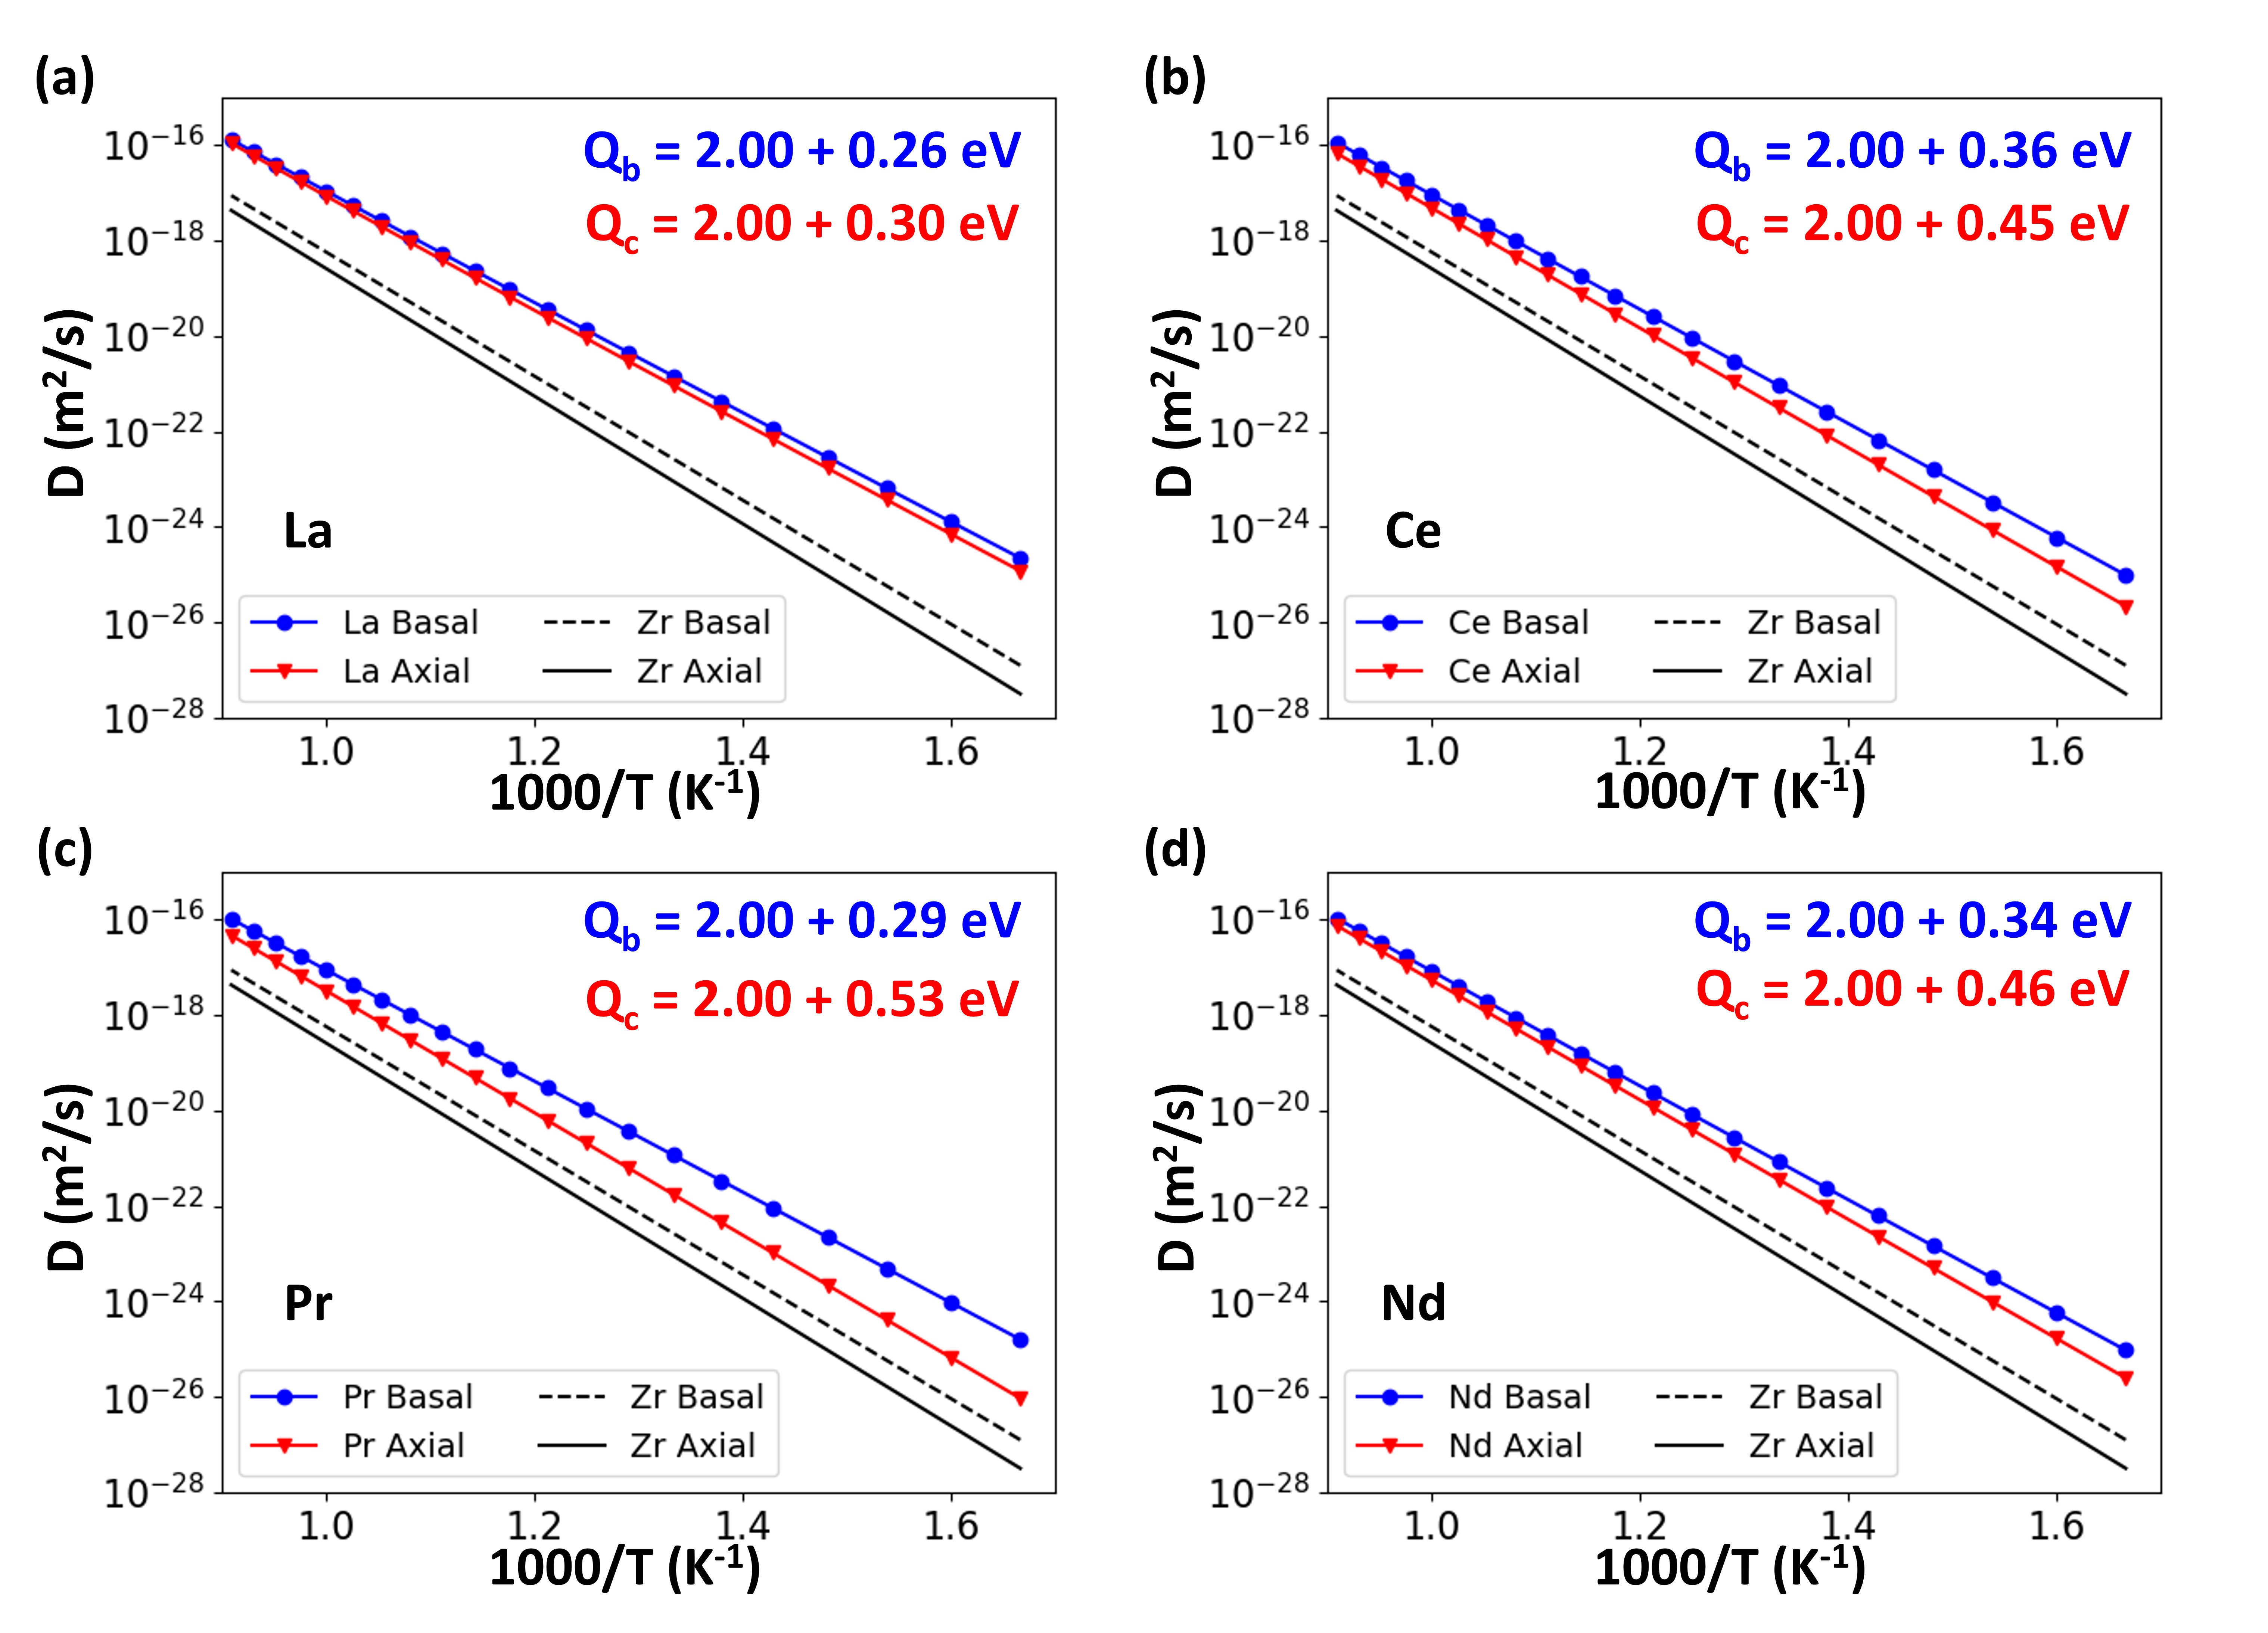
\includegraphics[width=\textwidth]{diffusivities_Q_updated.jpg}
%DIFDELCMD <     %%%
\DIFdelendFL \DIFaddbeginFL 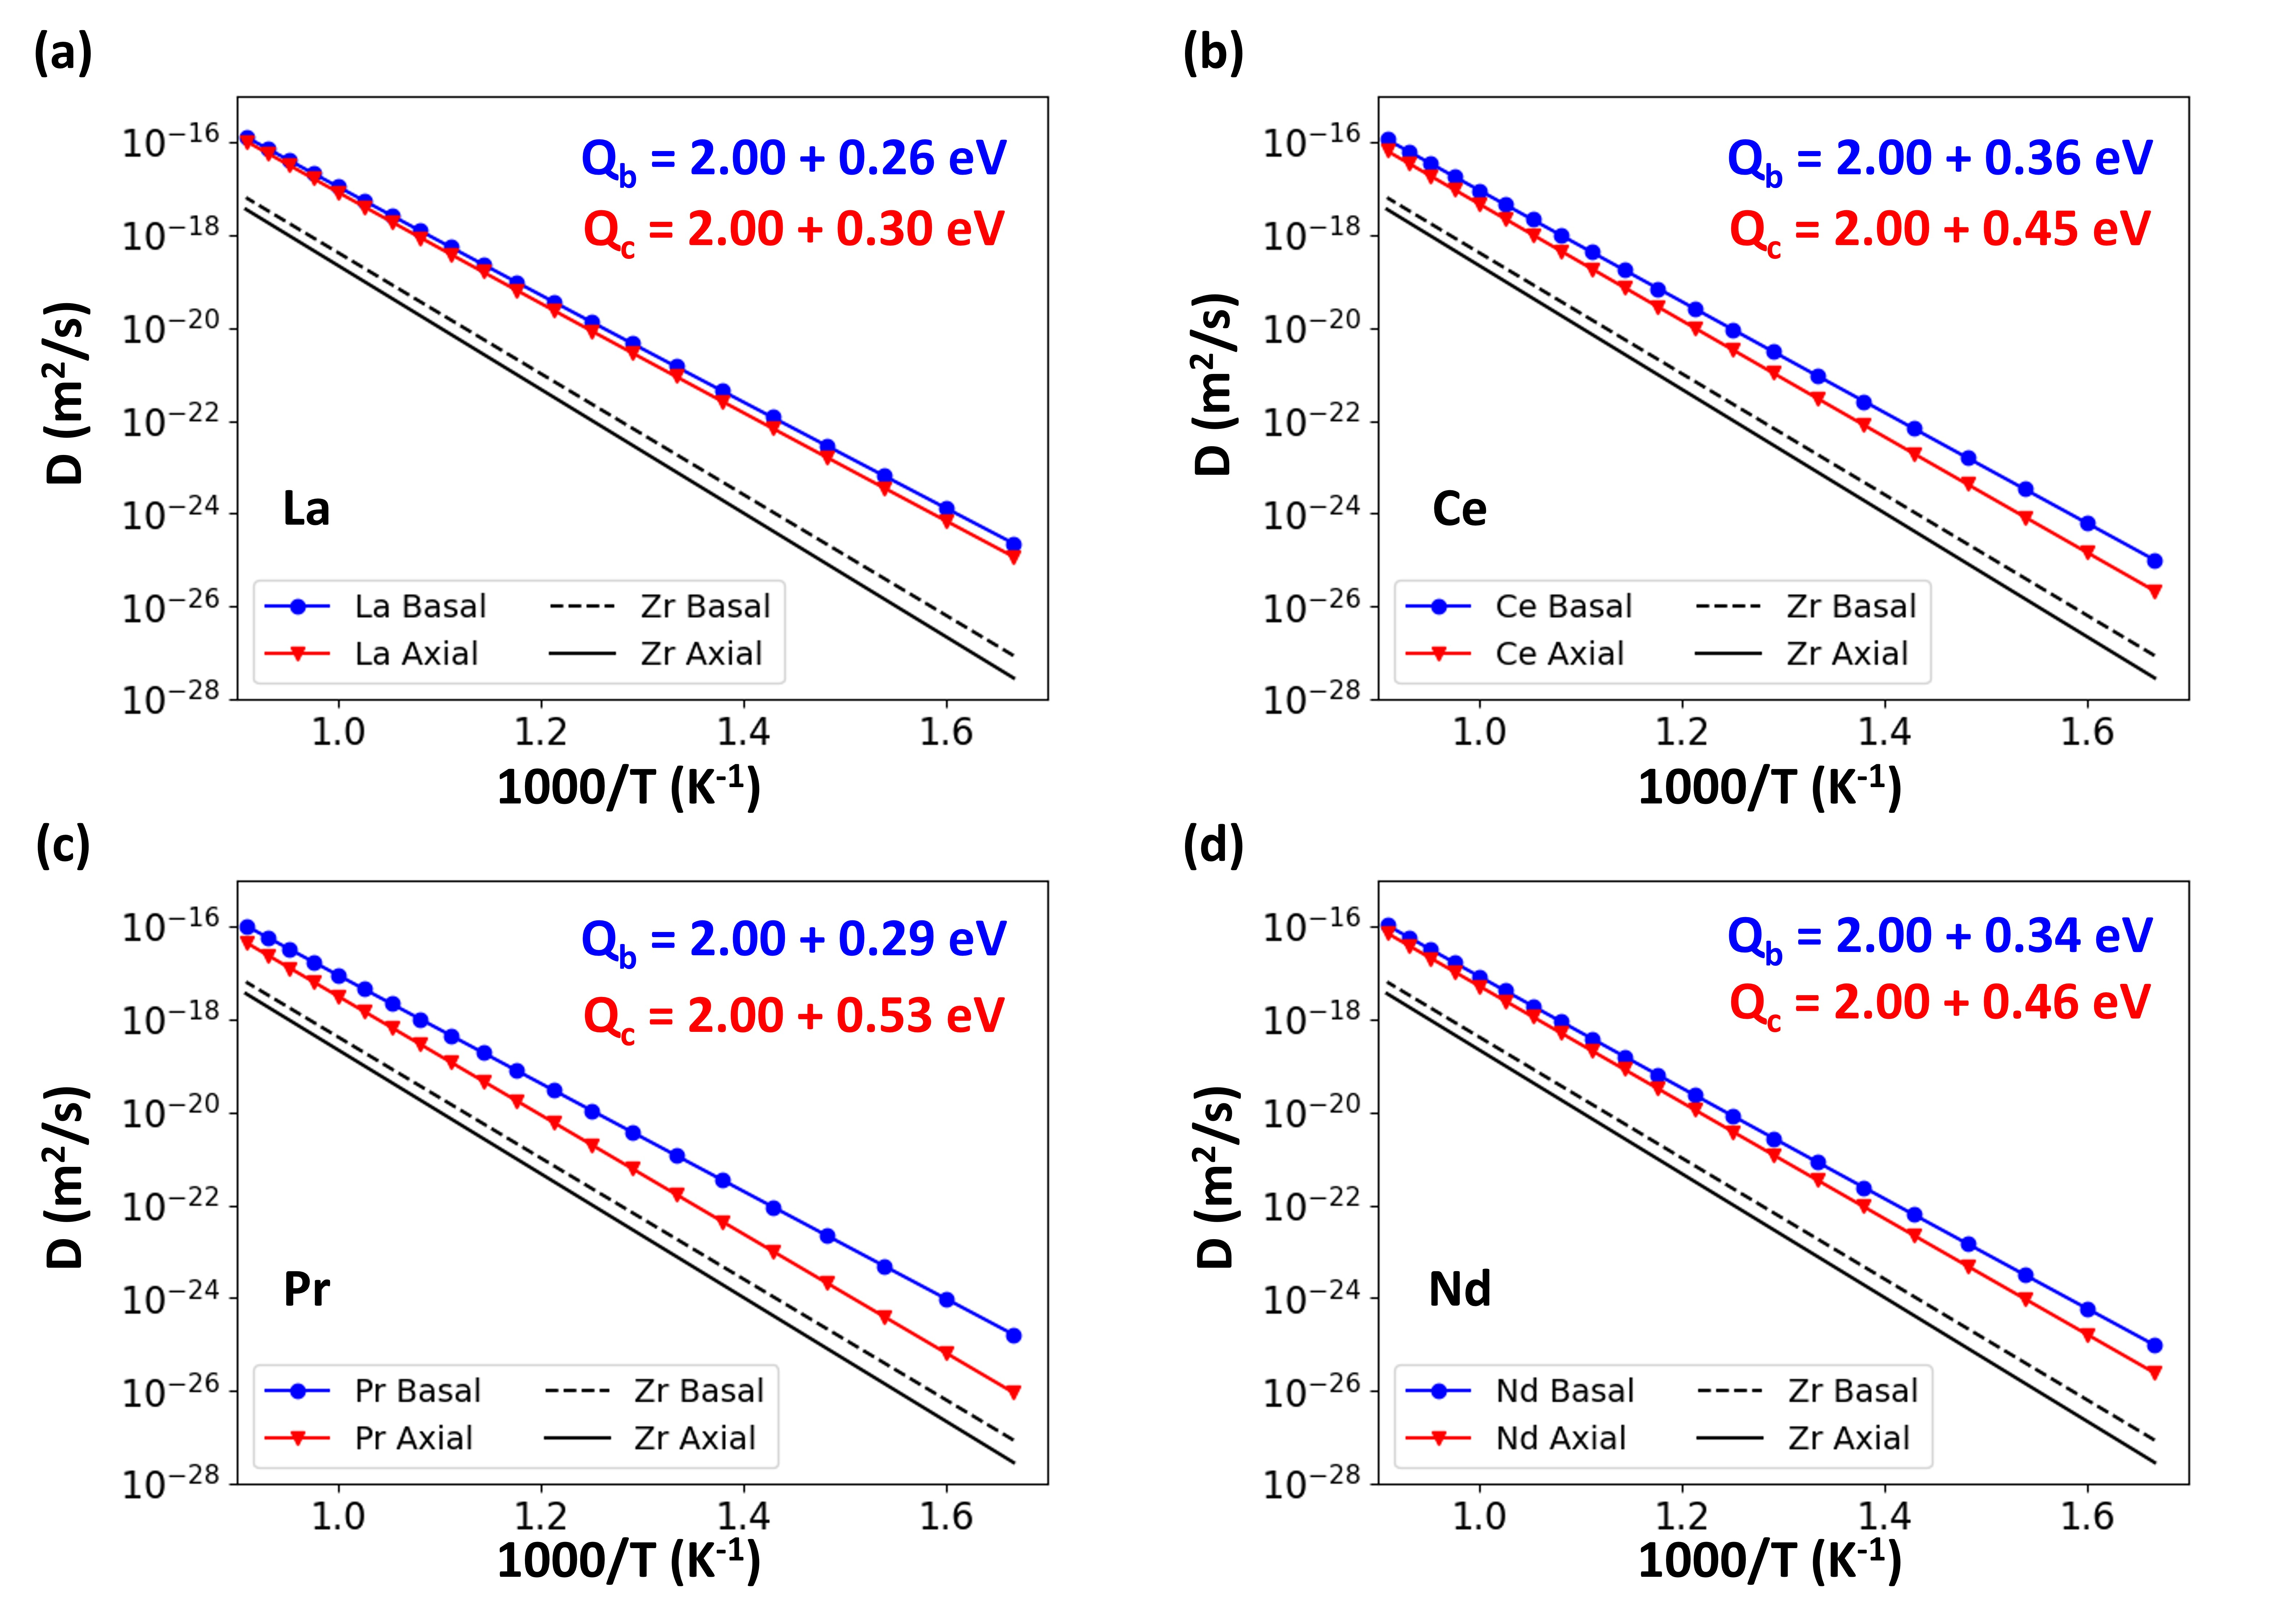
\includegraphics[width=0.9\textwidth]{5_diffusivities_Q_updated_added_f0.jpg}
    \DIFaddendFL \caption{The bulk diffusivities (D) of the four lanthanides La, Ce, Pr, and Nd in HCP-Zr are plotted versus inverse temperature in panels (a), (b), (c), and (d), respectively, at temperatures between 600 K and 1100 K. The lanthanide diffusivities in the basal planes (circle markers) and the corresponding activation barrier ($Q_b$) are in blue while the diffusivities along the c-axis (triangle markers) and the corresponding activation barrier ($Q_c$) are in red. The activation barriers shown are the sum of contributions from the vacancy formation energy (2 eV) and an effective migration barrier. %DIF < (binding and migration energies from all the considered configurations and jumps). 
    For comparison, the self-diffusivity in pure HCP-Zr is plotted in each panel using dashed and solid black lines for basal and axial directions, respectively.}
    \label{fig:diffusivities_ln}
\end{figure}

\begin{table}[h!]
    \centering
    \caption{The fitted activation energies ($Q$) and prefactors ($D_0$). The subscripts (b) and (c) denote diffusion along basal and c-axis directions, respectively.}
    \label{tab:arrhenius_fit}
    \begin{tabular}{c|c|c|c|c|c}
    \toprule
       & Zr (self-diffusion) & La & Ce & Pr & Nd  \\
       \hline
      $Q_b$ (eV) & \DIFdelbeginFL \DIFdelFL{2.572 }\DIFdelendFL \DIFaddbeginFL \DIFaddFL{2.579 }\DIFaddendFL &2.262 &2.358 & 2.292  & 2.342 \\
      $D_{0b} (\times10^{-6} m^2s^{-1})$ & \DIFdelbeginFL \DIFdelFL{5.2 }\DIFdelendFL \DIFaddbeginFL \DIFaddFL{4.1 }\DIFaddendFL & 2.5 & 6.7 & 3.1  &5.0 \\
      \hline
      $Q_c$ (eV) & \DIFdelbeginFL \DIFdelFL{2.649 }\DIFdelendFL \DIFaddbeginFL \DIFaddFL{2.644 }\DIFaddendFL &2.301 &2.450 &2.531   &2.460 \\
      $D_{0c}  (\times10^{-6} m^2s^{-1})$  &\DIFdelbeginFL \DIFdelFL{5.8 }\DIFdelendFL \DIFaddbeginFL \DIFaddFL{4.7 }\DIFaddendFL &2.9 &9.5 & 17.3  &12.2 \\
      \bottomrule
    \end{tabular}
\end{table}

\DIFaddbegin \FloatBarrier
\DIFaddend La is the fastest \DIFaddbegin \DIFadd{diffusing }\DIFaddend species and has the least anisotropic diffusion behavior with activation energies of 2.26 eV and 2.30 eV in the basal and axial directions, respectively. This low degree of anisotropy and the relatively fast diffusion along the c-axis is primarily because of the relatively low migration barrier of the pyramidal La-vacancy exchange jump ($E_m$=0.049 eV, \Cref{tab:jumps}). This jump contributes to the net diffusion of La in both basal and axial directions. On the other hand, Pr shows the highest degree of anisotropic diffusion with activation energies of 2.29 eV and 2.53 eV in the basal and axial directions, respectively. This can be explained by the relatively high migration barrier of the pyramidal Pr-vacancy exchange ($E_m$=0.158 eV, \Cref{tab:jumps}) compared to the three other species which translates into a slow diffusion along the c-axis. This does not significantly slow the diffusion of Pr in the basal plane because other jumps that contribute solely to the basal diffusion (1b'-1b', 1b'-1p, 1b'-2p, 1b'-4b, 1b'-4$\overline{b}$, 1b'-4p, and 1b'-6b in \Cref{tab:jumps_vac_oversized}) have relatively low migration barriers.

In summary, the diffusivities of La, Ce, Pr, and Nd in the basal plane in HCP-Zr are comparable to each other with activation energies between 2.26 and 2.36 eV. On the other hand, in the axial direction, the variation is larger. La is significantly the fastest species with an activation energy of 2.30 eV, while Pr is the slowest with an activation energy of 2.53 eV. Ce and Nd have intermediate values of 2.45 eV, and 2.46 eV, respectively. The diffusion of all lanthanides is faster than Zr self-diffusion in both the basal and axial directions. To facilitate this comparison, the four lanthanides' diffusivities are plotted together in \DIFdelbegin \DIFdel{\Cref{fig:diffusion_all_lanthanides} in \ref{app:dft_data}}\DIFdelend \DIFaddbegin \DIFadd{\Cref{fig:correlation_factors} in \ref{appendix_correlation}}\DIFaddend .

\FloatBarrier

\subsection{Solute Drag and Segregation Tendencies}
\label{subsection_drag}

In addition to diffusion coefficients, the vacancy drag ratios and partial diffusion coefficient ratios were calculated to obtain insight into the flux coupling and the segregation tendencies of lanthanides and vacancies in HCP Zr. The vacancy drag ratio ($G_V$) indicates if a solute diffuses in the same direction of the vacancy flux due to vacancy drag\DIFaddbegin \DIFadd{, }\DIFaddend $G_V > 0$\DIFaddbegin \DIFadd{, }\DIFaddend or diffuses in the opposite direction\DIFaddbegin \DIFadd{, }\DIFaddend $G_V < 0$ (known as the inverse Kirkendall effect (IKE) \cite{marwick_segregation_1978}). $G_V$ is defined by \Cref{eq:drag}.
\begin{equation}\label{eq:drag}
    G_V = \DIFdelbegin \DIFdel{\frac{L_{VB}}{L_{BB}}
}\DIFdelend \DIFaddbegin \DIFadd{\frac{L_{VB}^{(VB)}}{L_{BB}^{(VB)}}
}\DIFaddend \end{equation}
Another important quantity, the partial diffusion coefficient ratio $D_{pd}$, \DIFdelbegin \DIFdel{evaluates the solute diffusivity relative to the diffusivity }\DIFdelend \DIFaddbegin \DIFadd{describes the diffusion speed and direction of a solute relative to that }\DIFaddend of the host atoms (Zr) including the \DIFaddbegin \DIFadd{effect of }\DIFaddend flux coupling with vacancies \DIFaddbegin \DIFadd{\cite{messina_solute_2020, messina_exact_2014} }\DIFaddend and is given by \Cref{eq:pdc}.
\begin{equation}\label{eq:pdc}
    D_{pd} = \DIFdelbegin \DIFdel{\frac{(1-[B])}{[B]} }\DIFdelend \DIFaddbegin \DIFadd{\frac{(1-C_B)}{C_B} }\DIFaddend \frac{L_{VB}}{L_{AV}}
\end{equation}
$D_{pd}$ may indicate the tendency of enrichment or depletion of solute atoms at vacancy sinks \DIFdelbegin \DIFdel{, }\DIFdelend \DIFaddbegin \DIFadd{(}\DIFaddend e.g., grain boundaries\DIFdelbegin \DIFdel{. This quantity is closely related to the vacancy drag ratio and its value }\DIFdelend \DIFaddbegin \DIFadd{) \cite{messina_exact_2014}. The value of this quantity }\DIFaddend can be interpreted in three different regimes. The first regime is at $D_{pd} < 0$, when $L_{VB} > 0$ and $L_{AV}$ is always negative. This indicates solute enrichment at the sinks resulting from the diffusion of solute atoms in the same direction as the vacancy flux ($G_V > 0$). The second regime is at $D_{pd} > 1$ where solute depletion takes place at sinks due to favorable vacancy-solute exchange. In this scenario, solute atoms are moving in the opposite direction to the vacancy flux ($G_V < 0$) and are faster than the Zr host atoms. In the third regime ($0 < D_{pd} < 1$), solute enrichment is taking place at sinks even though there is no vacancy drag ($G_V < 0$). In this regime, both solute and host atoms are moving away from the sinks (opposite to the vacancy flux) \DIFdelbegin \DIFdel{but because }\DIFdelend \DIFaddbegin \DIFadd{and since }\DIFaddend the solute atoms are slower, the solute is effectively enriched at the sinks \DIFaddbegin \DIFadd{\cite{messina_exact_2014}}\DIFaddend . 

$G_V$ and $D_{pd}$ are plotted in the basal and axial directions in \Cref{fig:drag_ratios} at temperatures between 300 K and 1100 K. First\DIFaddbegin \DIFadd{, }\DIFaddend if we consider the diffusion in the basal planes in \Cref{fig:drag_ratios}(a), lanthanides have $G_V \approx 1$ at low temperatures (300 K) and $G_V$ decreases with temperature until it reaches a crossover temperature at T = 910, 1000, and 1030 K, for Nd, La, and Ce, respectively. Below these temperatures, lanthanide enrichment at the vacancy sinks driven by the vacancy drag is expected ($D_{pd} < 0$) as shown in \Cref{fig:drag_ratios}(c). While above these transition temperatures, lanthanides are no longer dragged by vacancies and they move in the opposite direction to the vacancy flux (\DIFdelbegin \DIFdel{IKE}\DIFdelend \DIFaddbegin \DIFadd{i.e., IKE takes place}\DIFaddend ). The lanthanides are still enriched at the sinks within a narrow temperature window when $ 0 < D_{pd} < 1$. Nd, La, and Ce are depleted at sinks when $ D_{pd} > 1$ for high temperatures above 930, 1030, and 1080 K, respectively.
Pr is always dragged by vacancies and enriched at sinks in the basal planes at all temperatures below 1100 K.



\begin{figure}[h!]
    \centering
    \DIFdelbeginFL %DIFDELCMD < 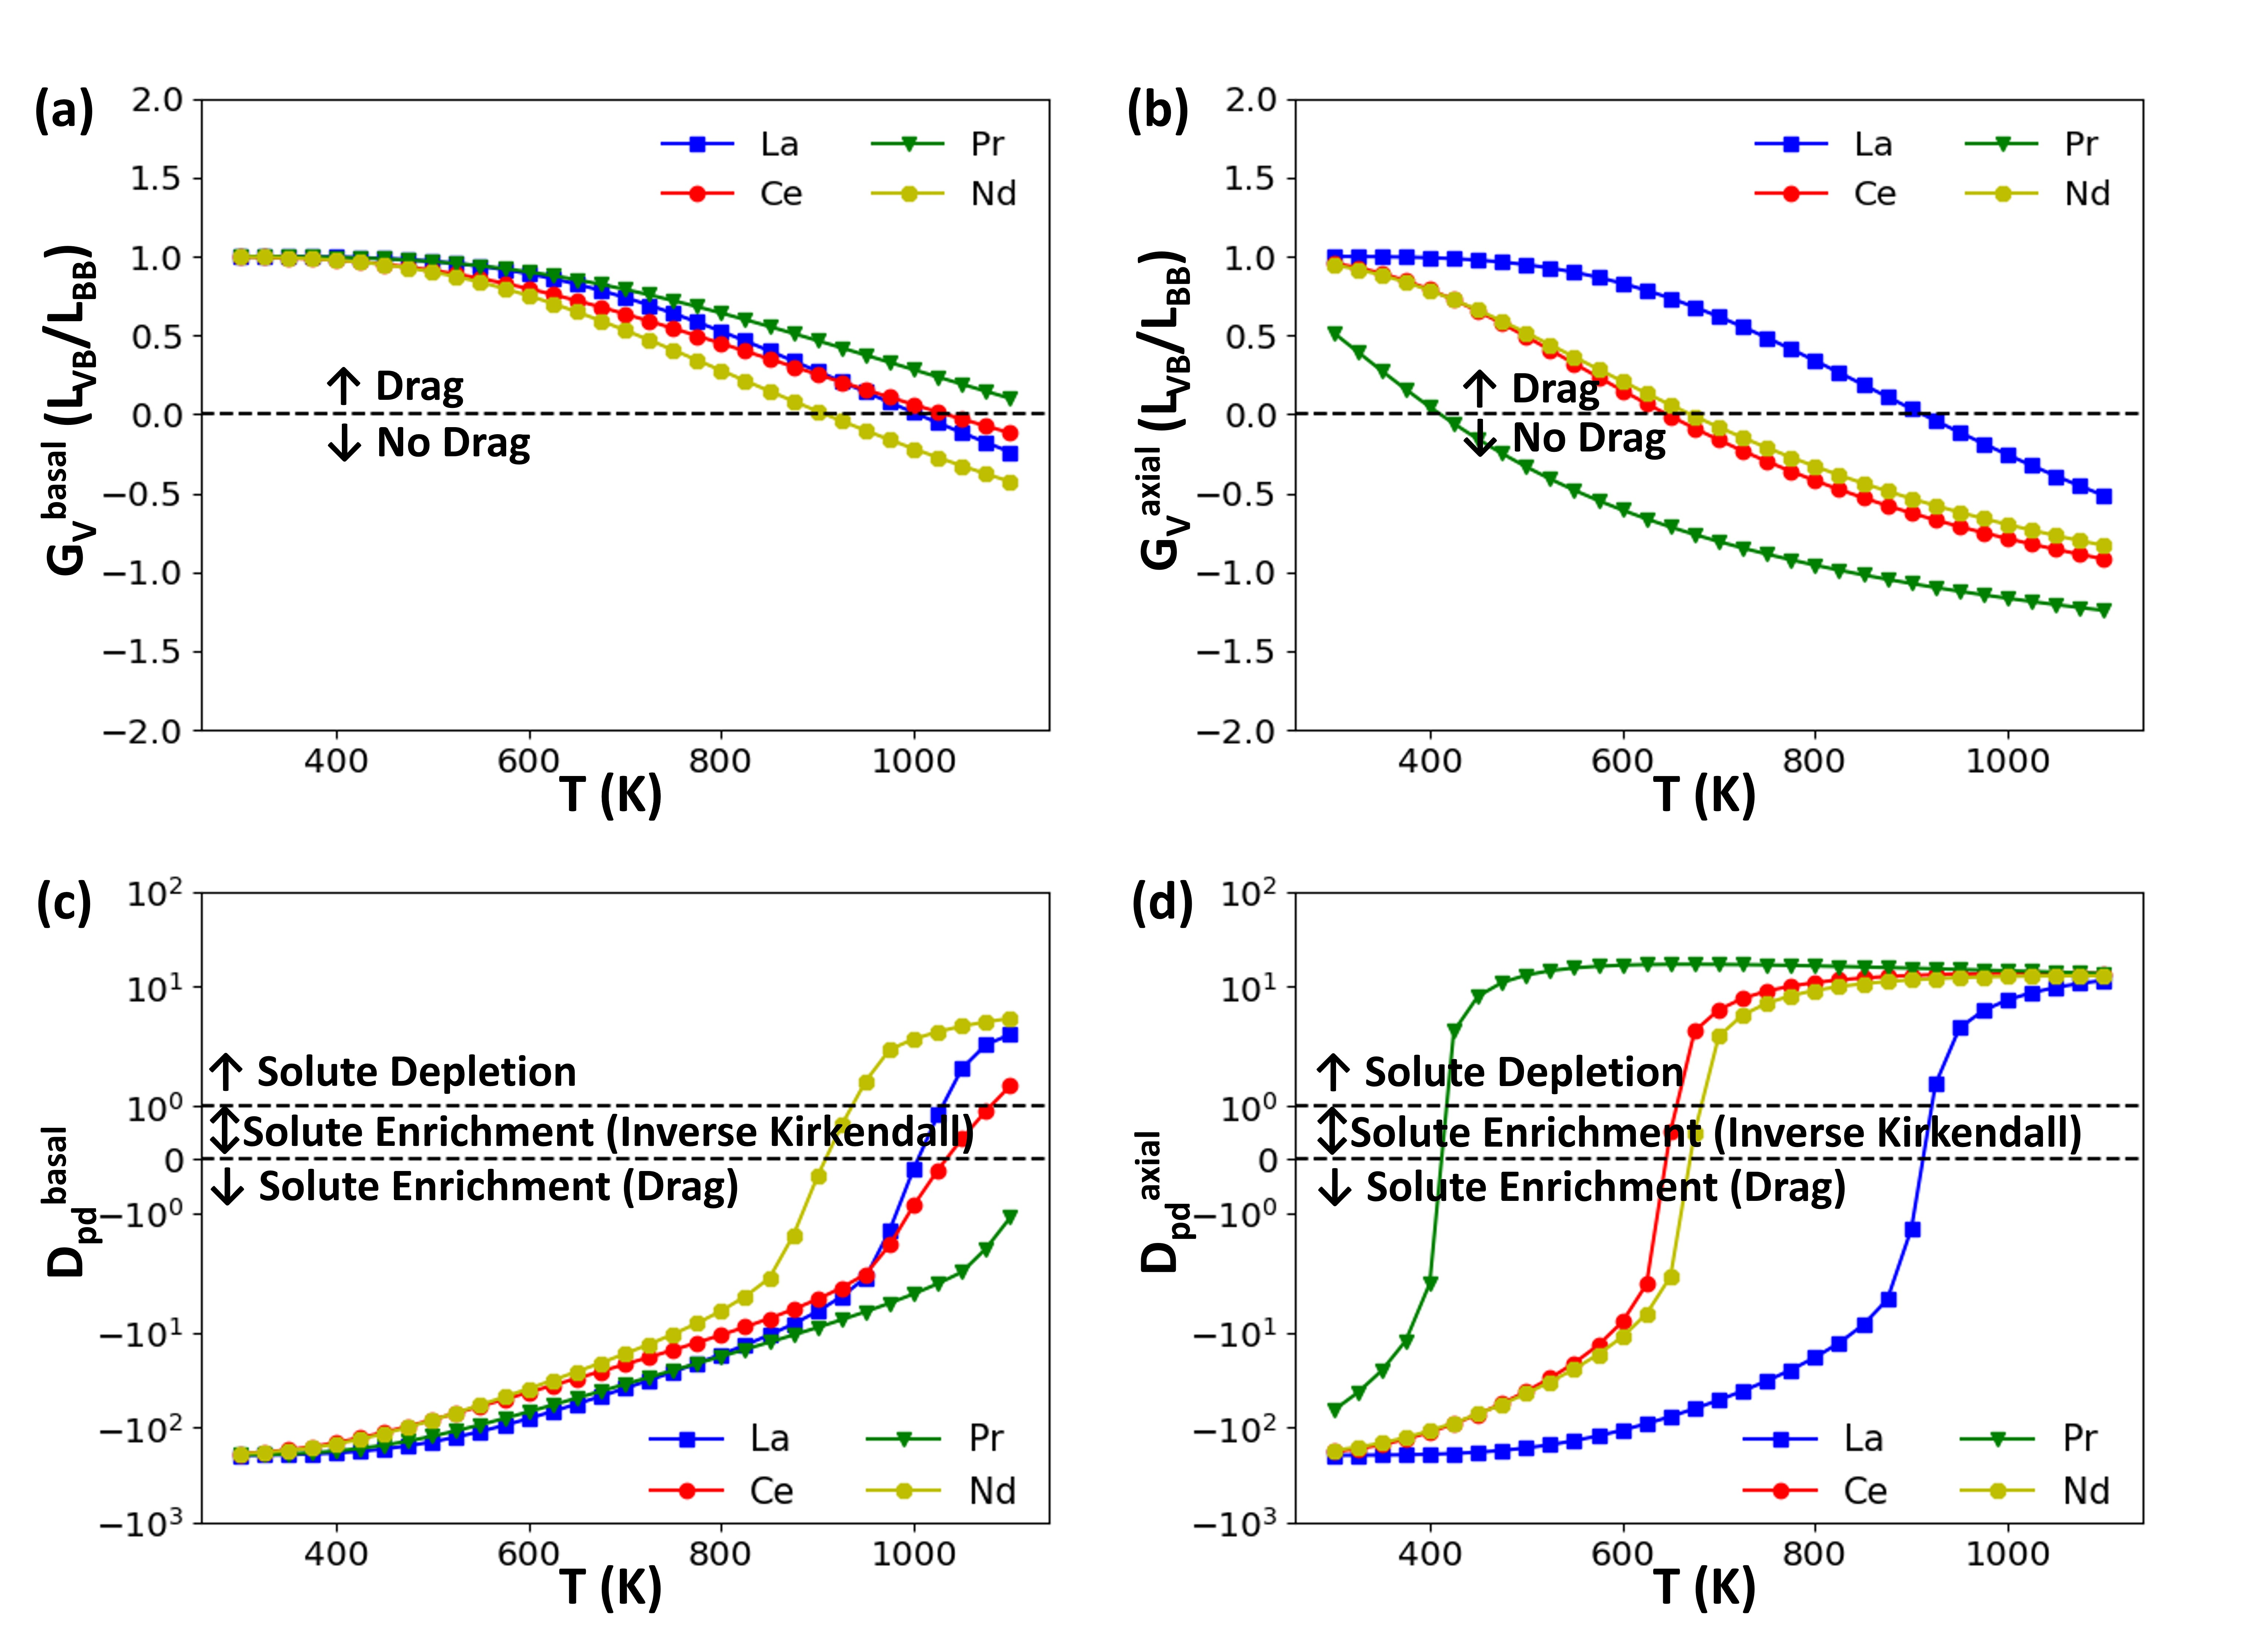
\includegraphics[width=\textwidth]{drag_pdc_basal_axial_updated.jpg}
%DIFDELCMD <     %%%
\DIFdelendFL \DIFaddbeginFL 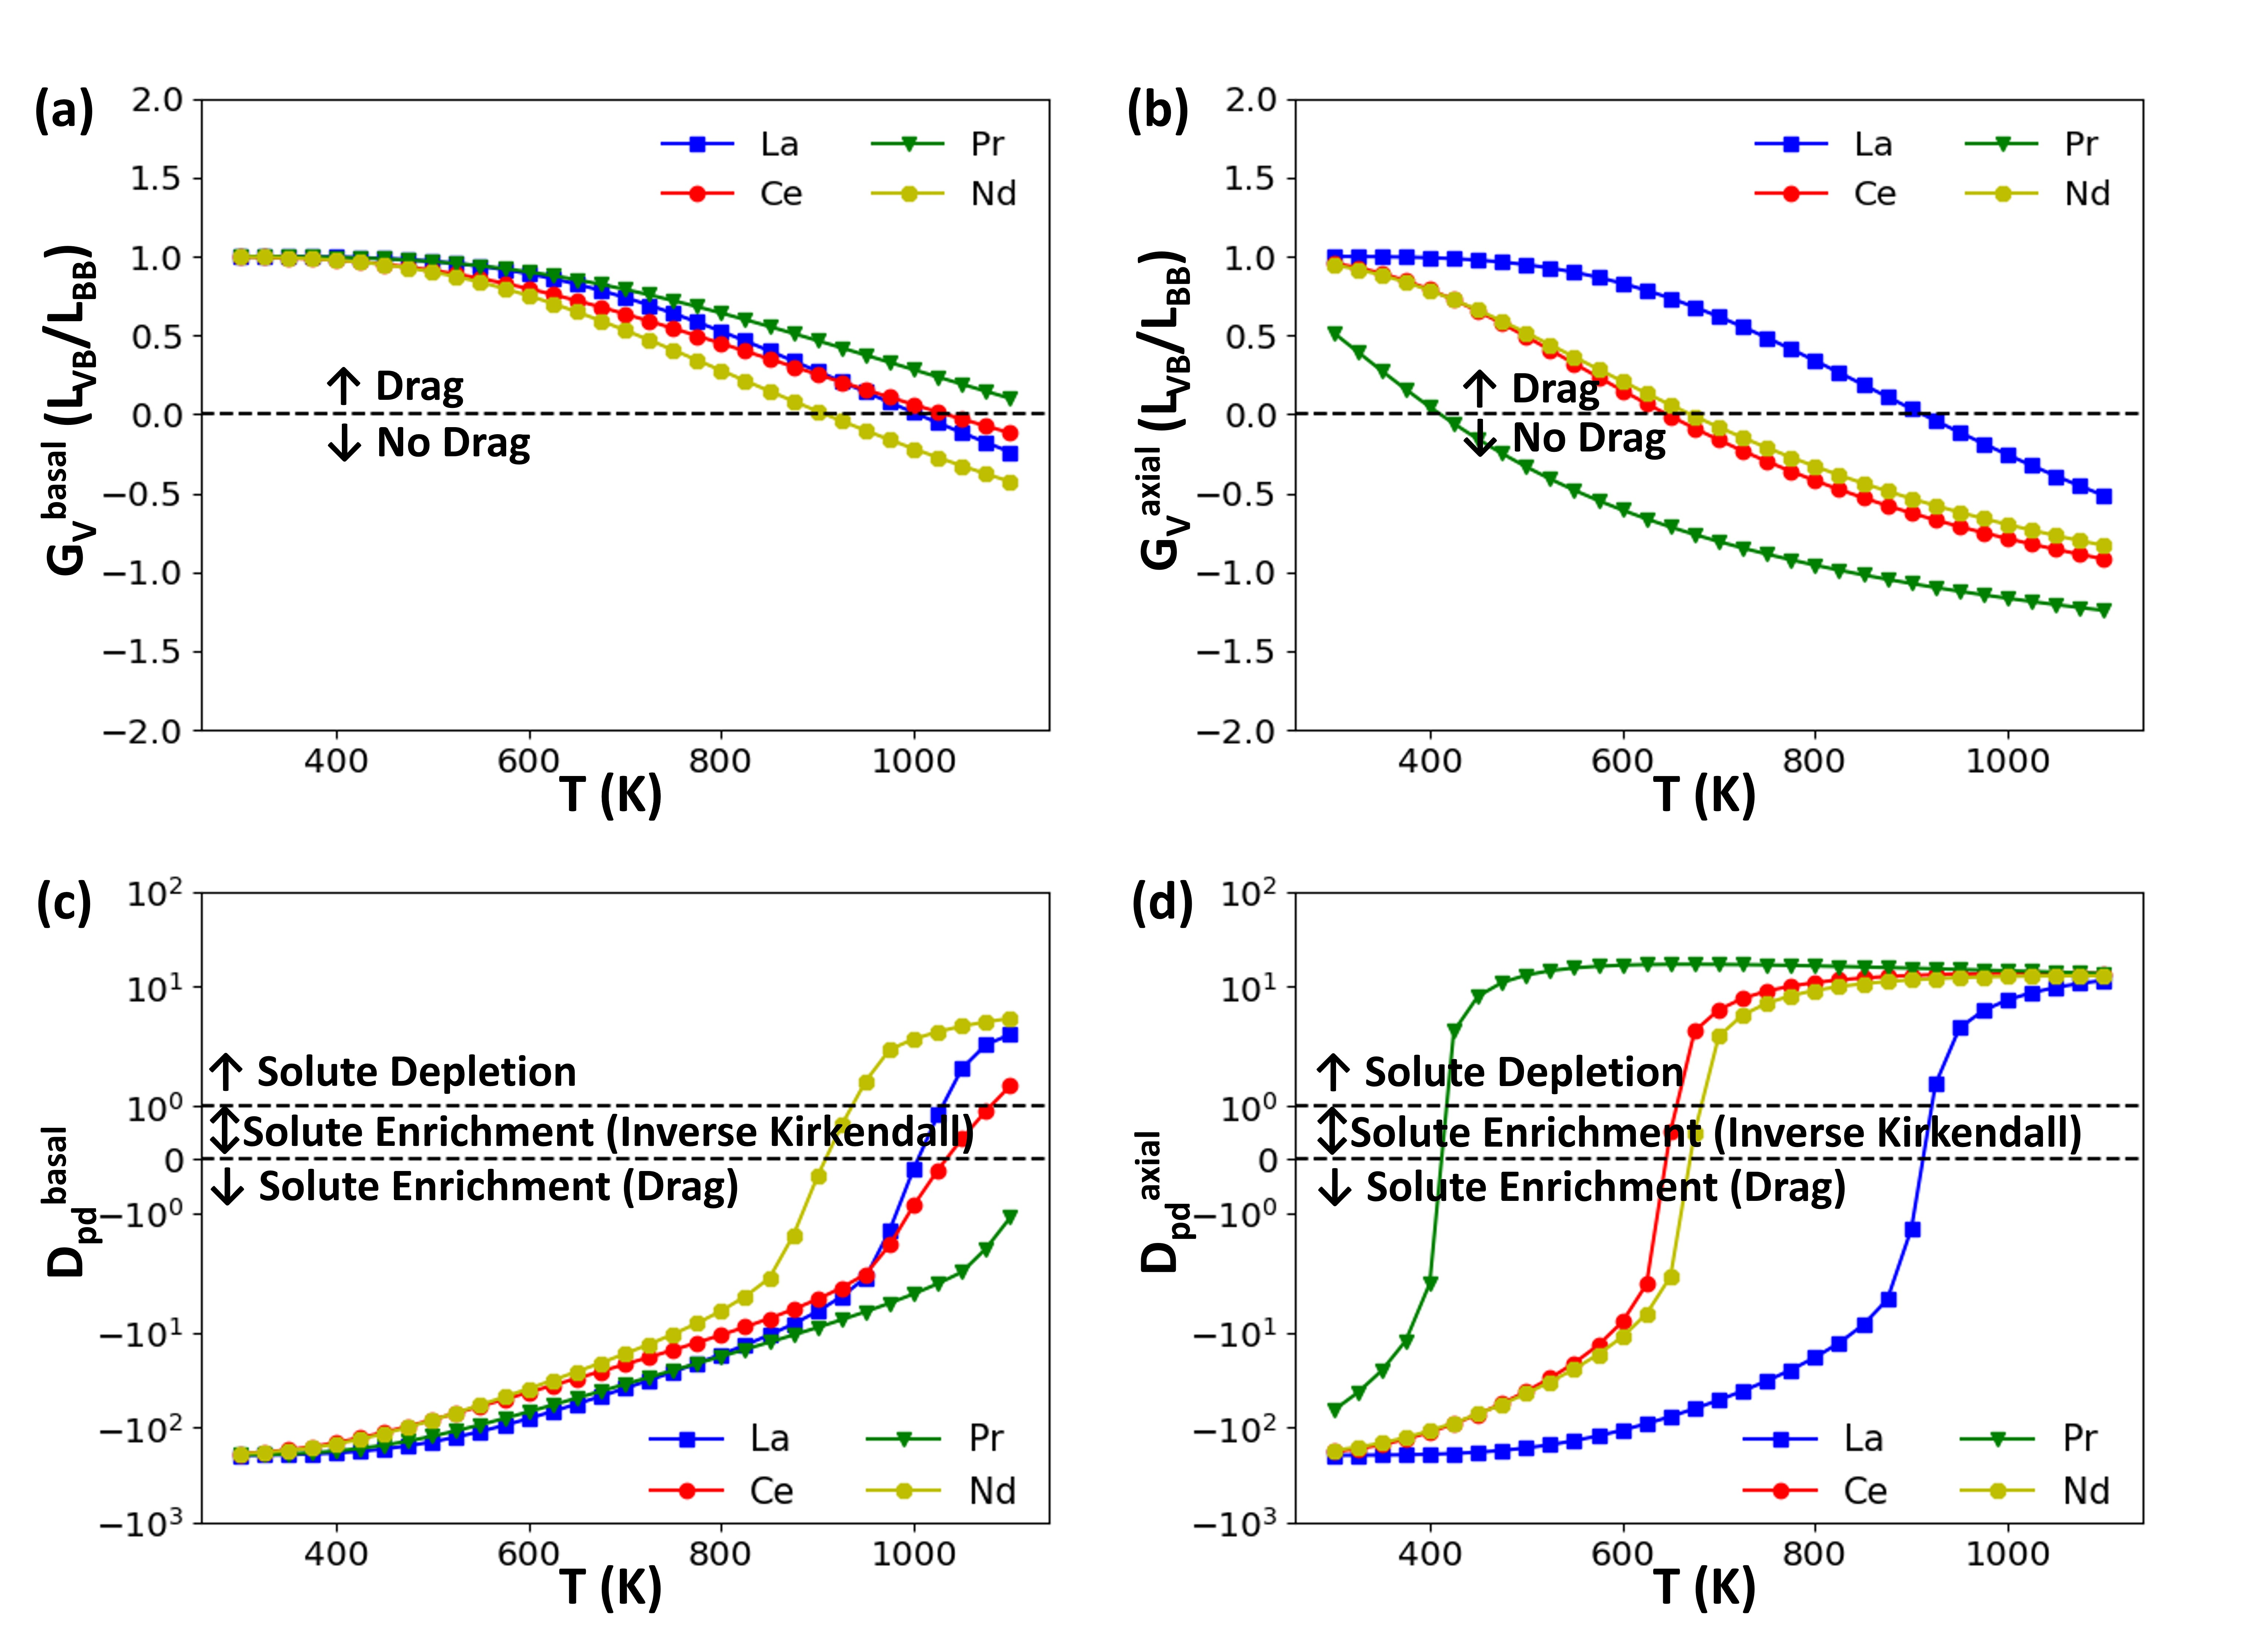
\includegraphics[width=0.9\textwidth]{6_drag_pdc_basal_axial_updated.jpg}
    \DIFaddendFL \caption{The vacancy drag ratios in the basal and axial directions ($G_V^{basal}$ and $G_V^{axial}$) are plotted versus temperature in (a) and (b), respectively, for La (blue), Ce (red), Pr (green), and Nd (yellow) in HCP Zr. The partial diffusion coefficient ratios in the basal and axial directions ($D_{pd}^{basal}$ and $D_{pd}^{axial}$) are plotted using the same color code in (c) and (d), respectively. $D_{pd}$ is calculated at the maximum solute concentration allowed in the dilute limit \DIFdelbeginFL \DIFdelFL{$[B] = 0.256 \%$ }\DIFdelendFL \DIFaddbeginFL \DIFaddFL{$[B] = 0.512$ ($at\%$) }\DIFaddendFL for La, Ce, and Pr, and \DIFdelbeginFL \DIFdelFL{$[B] = 0.258 \%$ }\DIFdelendFL \DIFaddbeginFL \DIFaddFL{$[B] = 0.516$ ($at\%$) }\DIFaddendFL for Nd (see \ref{appendix_partition}).}
    \label{fig:drag_ratios}
\end{figure}

Now, consider the diffusion in the axial (c-axis) direction in \Cref{fig:drag_ratios}, panels (b) and (d). Due to the low degree of anisotropy in La diffusion\DIFaddbegin \DIFadd{, }\DIFaddend as mentioned earlier in \cref{subsection_diffusivities}, it exhibits a similar drag behavior to that in the axial direction with strong vacancy drag and solute enrichment for a wide temperature range. The transition from vacancy drag to IKE and the change of segregation tendency from enrichment to depletion at sinks also occur at relatively high temperatures of T = 910 and 920 K, respectively. For the other three lanthanides with a higher degree of anisotropy, the vacancy-drag behavior in the axial direction is different from that in the basal planes. The main feature in the axial direction is that the vacancy drag of Pr, Ce, and Nd changes steeply with temperature as seen in \Cref{fig:drag_ratios}(b). Consequently, the transition from the enrichment to depletion regimes occurs at relatively lower temperatures in the axial direction as seen in \Cref{fig:drag_ratios}(d). For the most anisotropic case, Pr, the vacancy drag regime in the axial direction constitutes a relatively narrow temperature range below T = 410 K. On the other hand, Pr depletion at sinks is expected for all temperatures above T = 420 K. Ce and Nd have very similar segregation behavior in the axial direction where the transition temperatures from vacancy drag to IKE are 645 and 670 K, respectively, and the transition from enrichment to depletion occurs at temperatures of 655 and 680 K, for Ce and Nd, respectively.



\DIFdelbegin \DIFdel{Finally, to get an insight into the sink enrichment/depletion tendencies in a polycrystalline microstructure, we obtain an average of the transport coefficients along three crystallographic directions:
}\begin{displaymath}
   \DIFdel{L_{VB}^{av} = \frac{1}{3} ( L_{VB}^{[1 0 \overline{1} 0] } +  L_{VB}^{[0 1 \overline{1} 0]} +   L_{VB}^{[0 0 0 1]}) = \frac{2}{3}  L_{VB}^{basal} + \frac{1}{3}  L_{VB}^{axial}
   \label{av_LVB}
}\end{displaymath}%DIFAUXCMD
\DIFdel{and, similarly :
}\begin{displaymath}
    \DIFdel{L_{AV}^{av} = \frac{2}{3}  L_{AV}^{basal} + \frac{1}{3}  L_{AV}^{axial}
    \label{av_LAV}
}\end{displaymath}%DIFAUXCMD
\DIFdel{The $D_{pd}$ for the polycrystalline Zr from these two average transport coefficients was calculated for the four lanthanides and is plotted in \Cref{fig:pdc_average}. The resulting $D_{pd}$ versus temperature behavior is a left shift of the basal plane results. For Nd, La, and Ce, the transition temperatures from vacancy drag to the IKE regime are slightly lower than when only considering diffusion in the basal planes. For Pr, the axial contribution makes the transition to the depletion regime feasible at high temperatures above 1075 K, unlike the case of basal diffusion. It should be noted that in this treatment we neglect the contribution from diffusion along grain boundaries and we are assuming a random grain orientation without texture.
}%DIFDELCMD < 

%DIFDELCMD < \begin{figure}[h!]
%DIFDELCMD <     \centering
%DIFDELCMD <     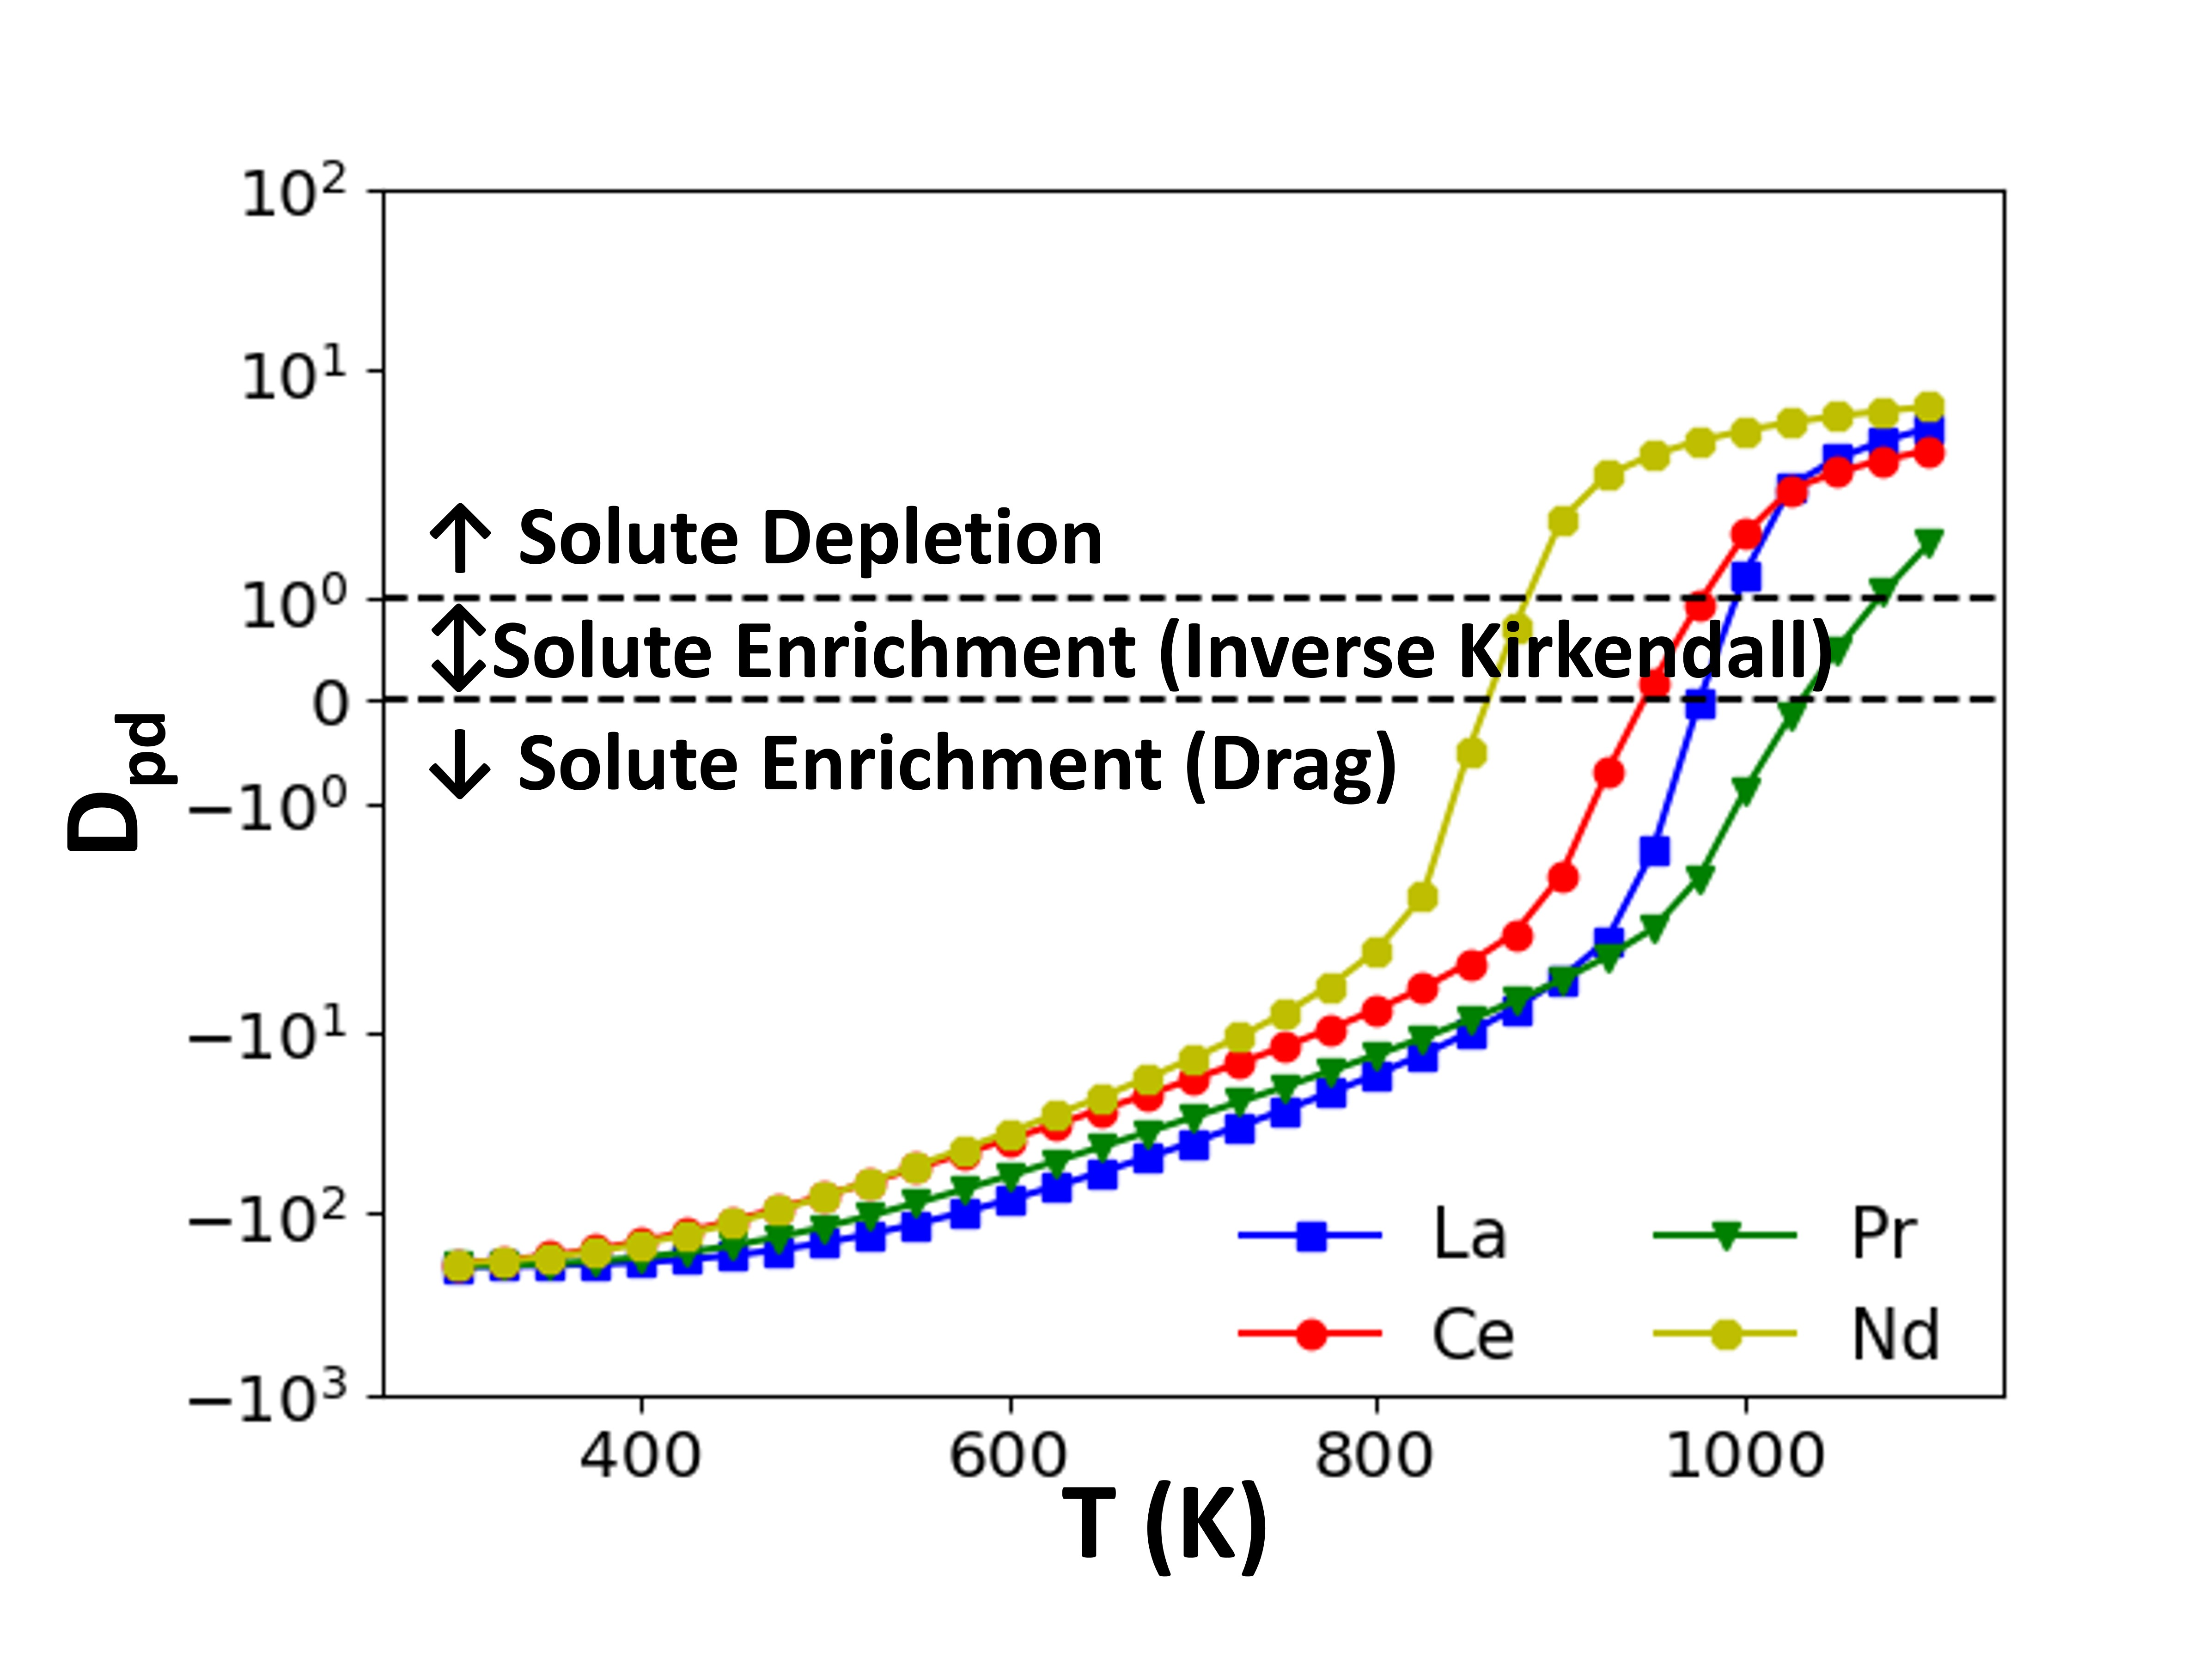
\includegraphics[width=0.8\textwidth]{pdc_av_updated.jpg}
%DIFDELCMD <     %%%
%DIFDELCMD < \caption{%
{%DIFAUXCMD
\DIFdelFL{Expected partial diffusion coefficient ratios for lanthanides in polycrystalline (isotropic) HCP Zr.}}
    %DIFAUXCMD
%DIFDELCMD < \label{fig:pdc_average}
%DIFDELCMD < \end{figure}
%DIFDELCMD < 

%DIFDELCMD < %%%
\DIFdelend \FloatBarrier

\section{Discussion}

\subsection{Vacancy-mediated diffusion vs. experimental measurements}
The diffusivities of lanthanides we report in this paper are considered the \DIFdelbegin \DIFdel{first of a kind}\DIFdelend \DIFaddbegin \DIFadd{first-of-a-kind}\DIFaddend . To the best of our knowledge, there \DIFdelbegin \DIFdel{have not been any atomistic calculations }\DIFdelend \DIFaddbegin \DIFadd{is only one other publication by Wang et al.\cite{wang_first_2019} that investigated the diffusion }\DIFaddend of these species in HCP Zr up to the date of publishing this work\DIFdelbegin \DIFdel{except for one study by Wang et al. that }\DIFdelend \DIFaddbegin \DIFadd{. This study }\DIFaddend considered the diffusion of Ce in HCP Zr using DFT and the simplified 8-frequency model\DIFdelbegin \DIFdel{\cite{wang_first_2019}. However}\DIFdelend \DIFaddbegin \DIFadd{. Our calculated Ce diffusivity in HCP-Zr and the results reported by Wang et al.\cite{wang_first_2019} show excellent agreement, as shown in Figure \ref{fig:ce_nd_exp}. Also}\DIFaddend , there are two experimental measurements of lanthanide diffusivities in HCP Zr in the literature that we can utilize for comparison. The \DIFaddbegin \DIFadd{experiment by Helmreich \cite{helmreich_diffusion_2014} employed a diffusion couple to obtain the Nd diffusivity from concentration profiles in HCP Zr. The reported diffusivities from Helmreich do not agree with the data from this work. Although the magnitude of the Nd diffusivity is comparable at T = 825 K, the difference in activation energies is very significant. The activation energy reported by Helmreich is 0.385 eV, which is too low compared to the activation energies reported in this work (2.34 eV and 2.46 eV, for basal and axial directions, respectively). However, it should be noted that the diffusivities reported by Helmreich are interdiffusion coefficients which are composition-dependent and involve both species (Zr and Nd). In contrast, the diffusion coefficients computed in this work are composition-independent and are analogous to tracer diffusion coefficients. Thus, the difference in activation energies is expected. The }\DIFaddend study by Paul et al. \cite{paul_diffusion_1968} measured the Ce diffusivity in $\alpha$ and $\beta$ \DIFdelbegin \DIFdel{zirconium }\DIFdelend \DIFaddbegin \DIFadd{Zr }\DIFaddend phases by using the \DIFaddbegin \DIFadd{residual activity technique with the }\DIFaddend $^{141}$Ce isotope\DIFdelbegin \DIFdel{in the residual activity technique}\DIFdelend \DIFaddbegin \DIFadd{. The Ce concentration in the sample was not reported explicitly in that study}\DIFaddend . The experimental data obtained by Paul et al. \cite{paul_diffusion_1968} for the $\alpha$-Zr HCP phase is plotted in \Cref{fig:ce_nd_exp} and compared to the results presented in this work. \DIFdelbegin \DIFdel{We find that there is a large disagreement in both the magnitude and the slope (activation barrier). The experiment by Helmreich \cite{helmreich_diffusion_2014} employed a diffusion couple to obtain the Nd diffusivity from concentration profiles }\DIFdelend \DIFaddbegin \DIFadd{To the best of our knowledge, this study by Paul et al. \cite{paul_diffusion_1968} is the only tracer diffusion experiment for a lanthanide in Zr, making the comparison of our calculated diffusivities meaningful. The activation barrier for Ce diffusion }\DIFaddend in HCP Zr \DIFdelbegin \DIFdel{. The reported diffusivities from Helmreich also do not agree with the data from this work. Although the magnitude of the Nd diffusivity is comparable at T = 825 K, the difference in activation energies is very significant}\DIFdelend \DIFaddbegin \DIFadd{reported by Paul et al. is 1.10 eV \cite{paul_diffusion_1968}. This value is significantly lower than the activation energies reported in this work: 2.36 eV and 2.45 eV, for basal and axial directions, respectively}\DIFaddend . 

\begin{figure}[h!]
    \centering
    \DIFdelbeginFL %DIFDELCMD < 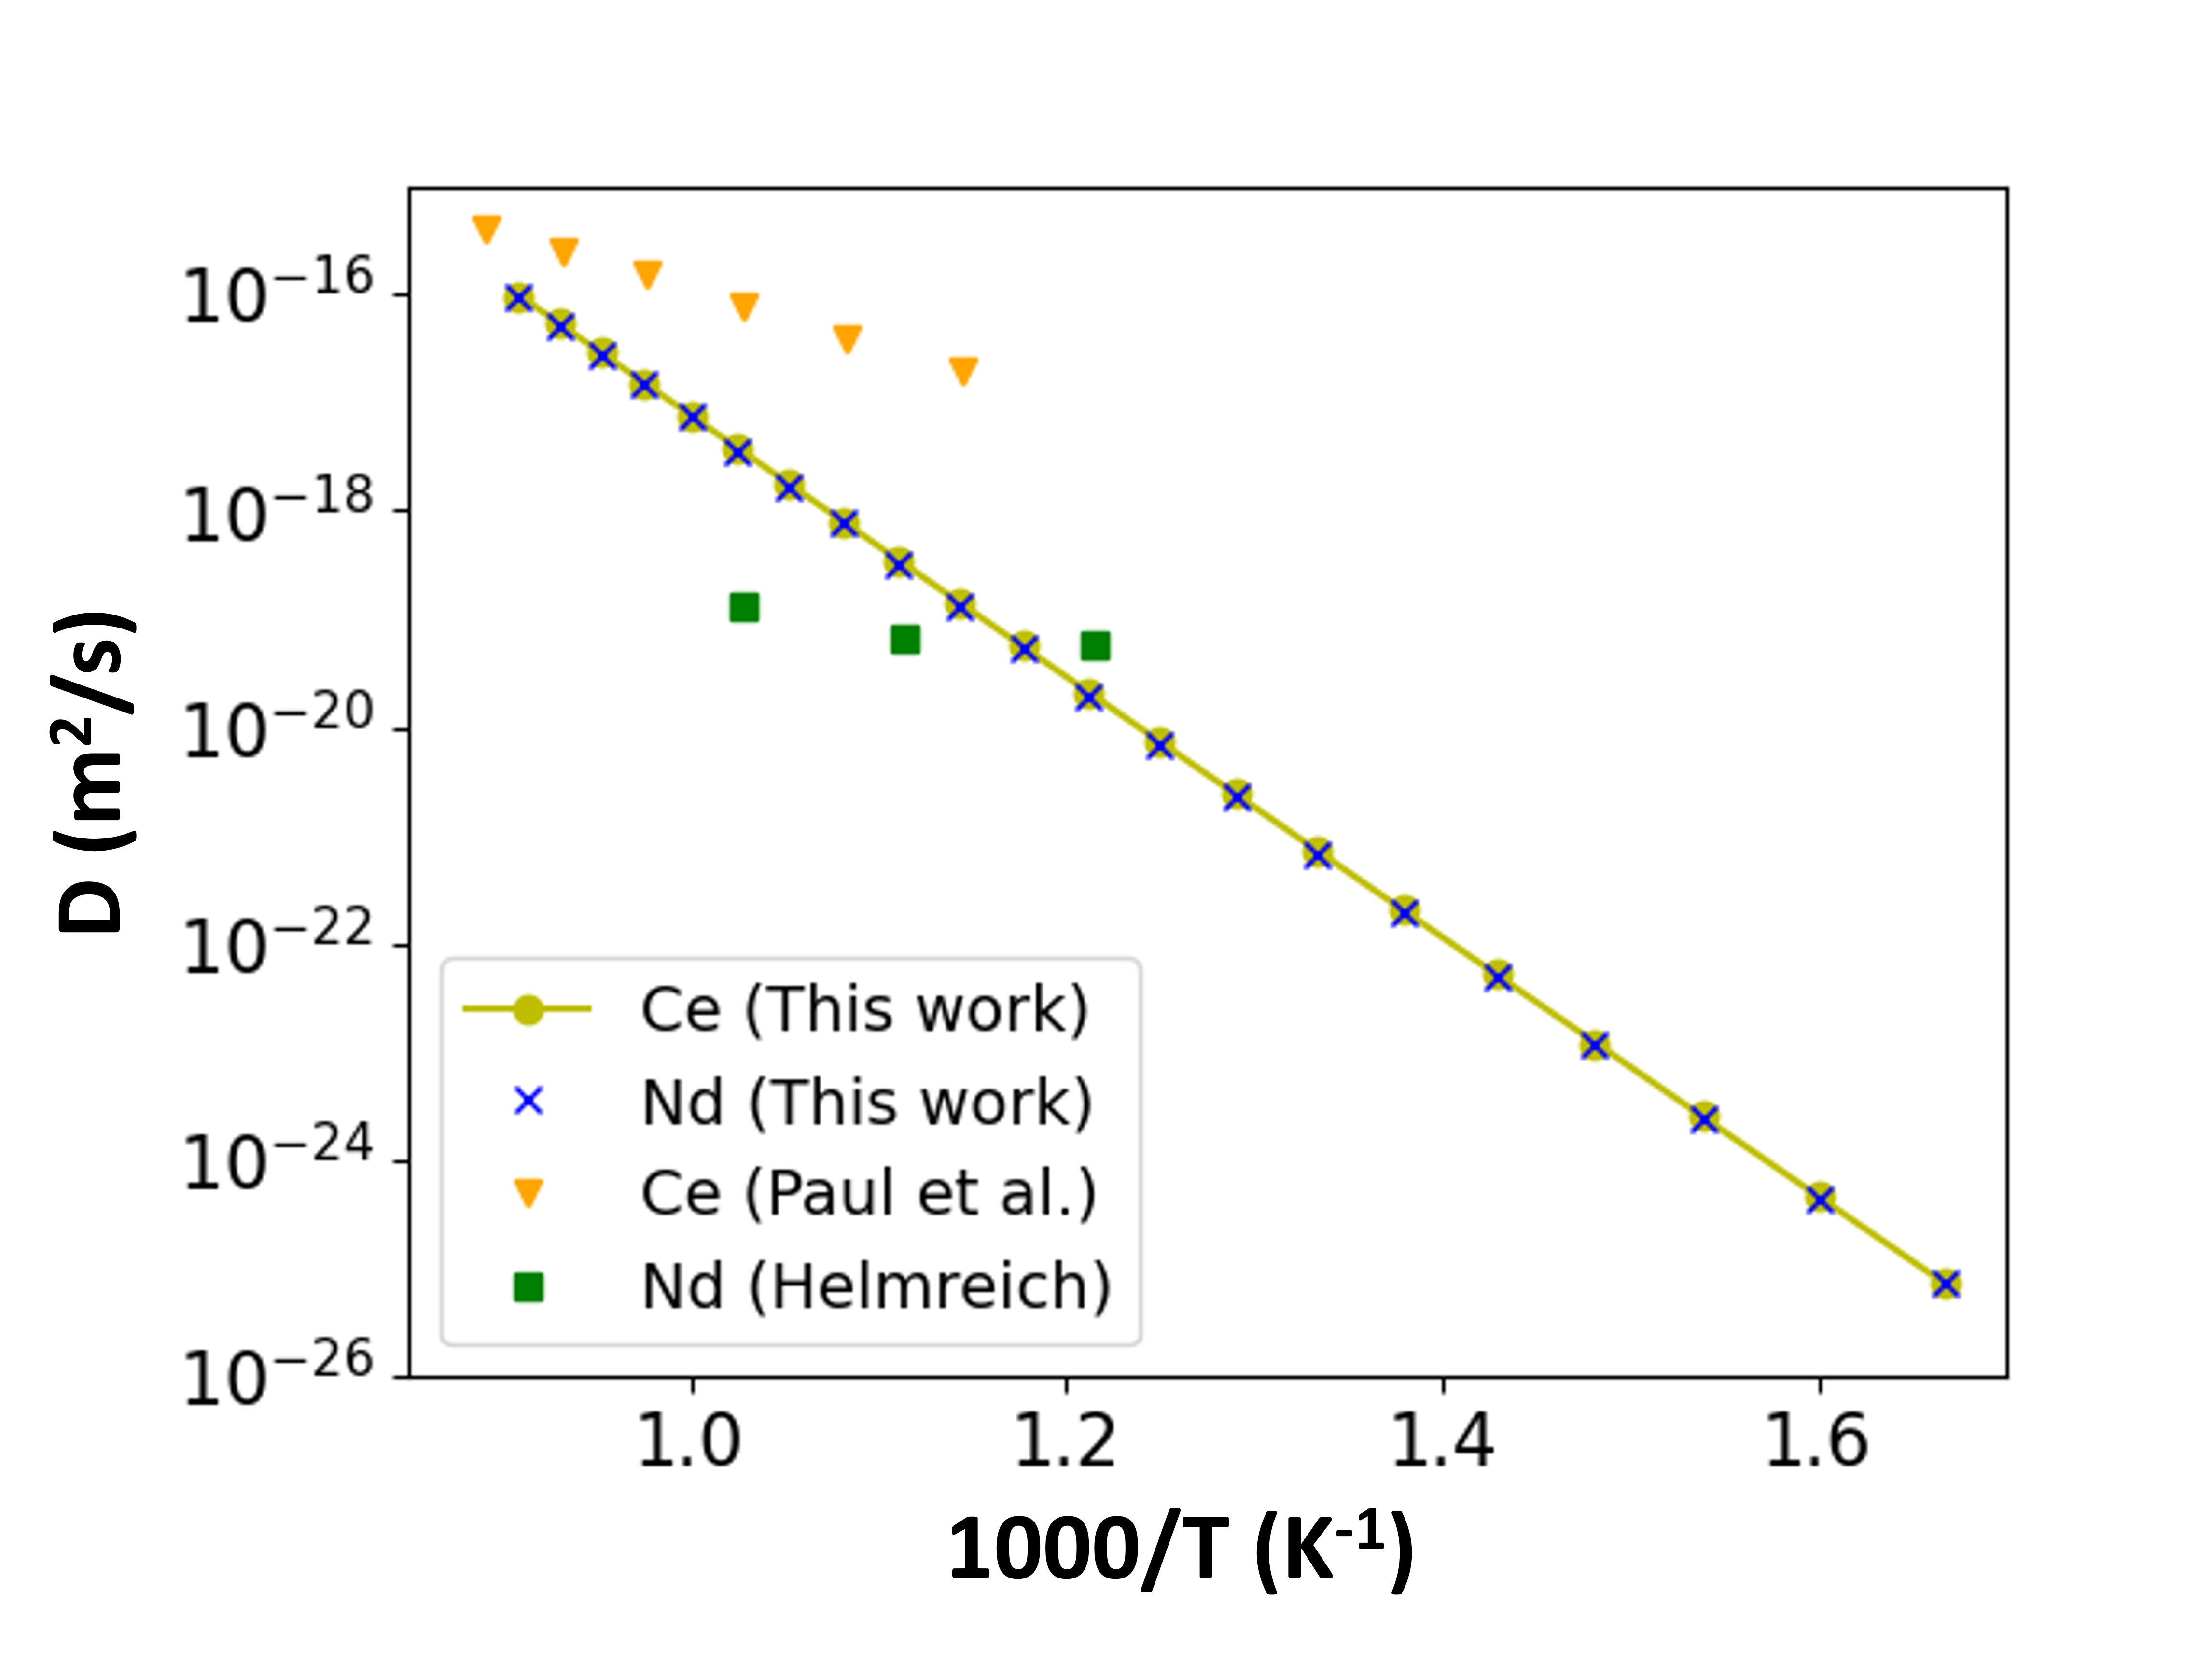
\includegraphics[width=0.8\textwidth]{ce_nd_diff_exp_updated.jpg}
%DIFDELCMD <     %%%
\DIFdelendFL \DIFaddbeginFL 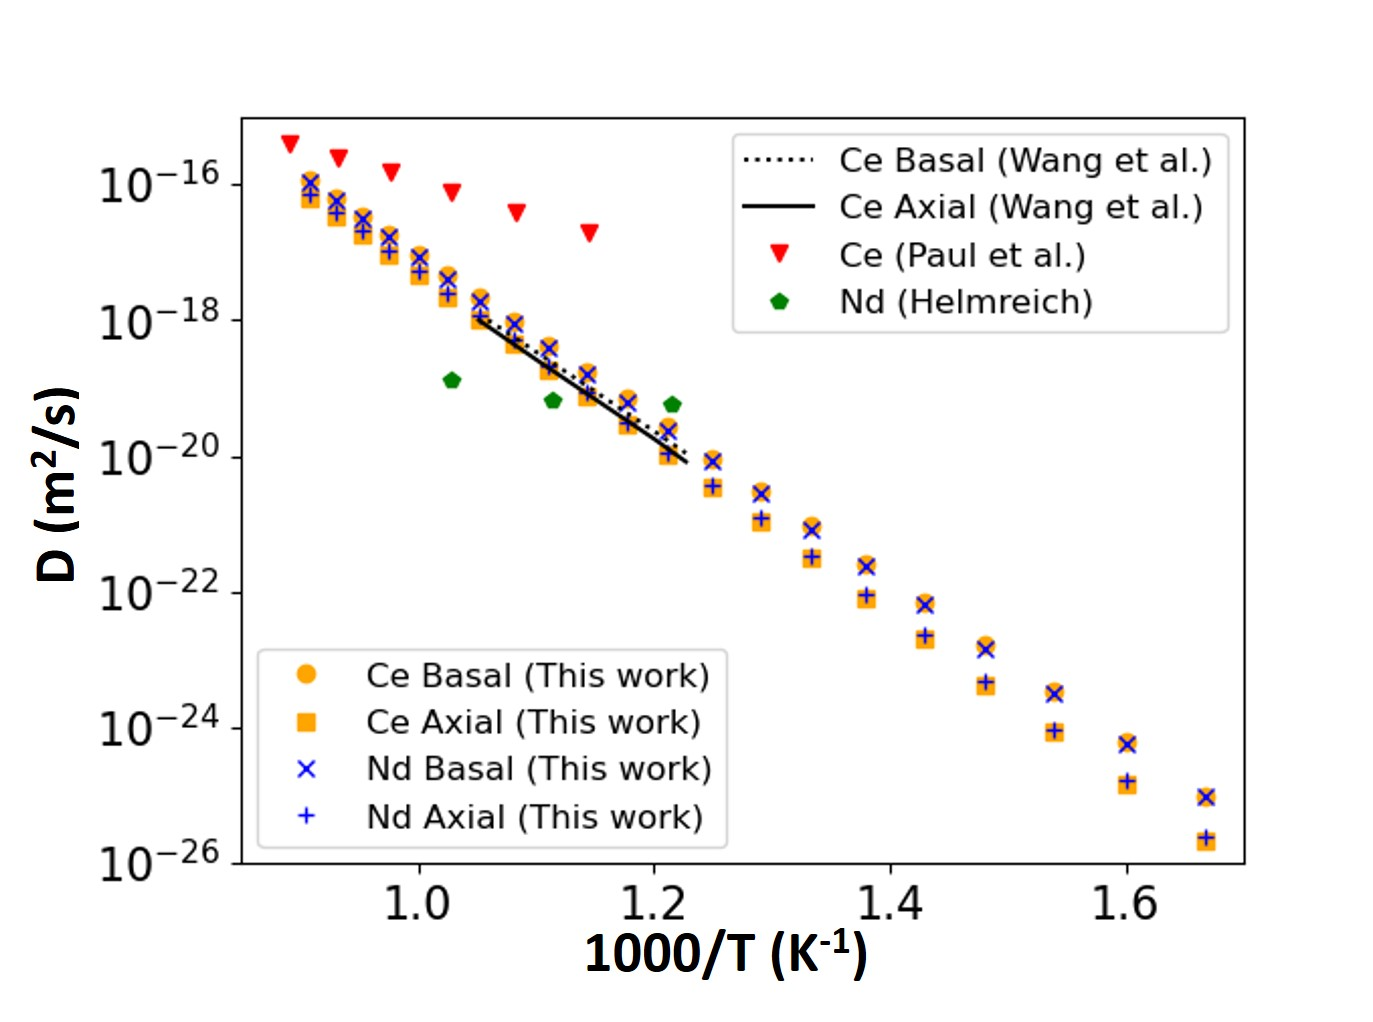
\includegraphics[width=0.7\textwidth]{8_ce_nd_diff_exp_8freq.jpg}
    \DIFaddendFL \caption{The average (isotropic) bulk diffusivity of Ce and Nd in HCP Zr compared to \DIFaddbeginFL \DIFaddFL{theoretical 8-frequency model results by Wang et al. \cite{wang_first_2019} and }\DIFaddendFL experimental results \DIFdelbeginFL \DIFdelFL{from }\DIFdelendFL \DIFaddbeginFL \DIFaddFL{by }\DIFaddendFL Paul \DIFaddbeginFL \DIFaddFL{et al. }\DIFaddendFL \cite{paul_diffusion_1968} and Helmreich \cite{helmreich_diffusion_2014}. \DIFdelbeginFL \DIFdelFL{The average diffusivity (D) is calculated similarly to Equations \ref{av_LVB} and \ref{av_LAV} by averaging the basal and axial contributions as follows: $D^{av} = \frac{2}{3} D^{basal} + \frac{1}{3} D^{axial}$}\DIFdelendFL }
    \label{fig:ce_nd_exp}
\end{figure}

Assuming that the samples used \DIFdelbegin \DIFdel{in the two studies \cite{paul_diffusion_1968, helmreich_diffusion_2014} }\DIFdelend \DIFaddbegin \DIFadd{by Paul et al. \cite{paul_diffusion_1968} }\DIFaddend are of high purity and that impurity diffusion does not affect the results, the comparison of our calculations to their results suggests that the vacancy mechanism \DIFaddbegin \DIFadd{alone }\DIFaddend may not be sufficient to describe the diffusion of lanthanides in HCP Zr. This may require accounting for interstitial diffusion mechanisms and/or grain boundary diffusion, especially in polycrystalline Zr. Even though interstitials have significantly higher formation energies than substitutionals, they may play a role in diffusive processes, especially at elevated temperatures. However, \DIFdelbegin \DIFdel{we find that }\DIFdelend the interstitial formation energies are at least 2 eV higher than the substitutional formation energies for Ce and Nd. \DIFaddbegin \DIFadd{We performed additional DFT calculations utilizing the same methodology presented above and found that the formation energies of Ce and Nd interstitials in octahedral sites are 2.81 and 4.00 eV, respectively. This is relatively high compared to the substitutional formation energies of 0.45 and 0.59 eV for Ce and Nd, respectively. }\DIFaddend Therefore, we suggest that the very low activation energies reported in experiments \DIFdelbegin \DIFdel{\cite{paul_diffusion_1968, helmreich_diffusion_2014} }\DIFdelend \DIFaddbegin \DIFadd{\cite{paul_diffusion_1968} }\DIFaddend cannot be explained by interstitial diffusion\DIFaddbegin \DIFadd{, }\DIFaddend but are most likely due to grain boundary diffusion. The grain boundary diffusion may be the dominant diffusion mechanism, especially at lower temperatures\DIFdelbegin \DIFdel{but }\DIFdelend \DIFaddbegin \DIFadd{. However, }\DIFaddend this also depends on the microstructure and grain boundary orientations. Both interstitial diffusion and grain boundary diffusion are outside the scope of this paper but will be explored in future work. Additional experimental investigations of the diffusion of lanthanides in single or pseudo-single crystals are required to experimentally validate the reported diffusivities calculated here.

\subsection{HCP Zr as an interdiffusion barrier in nuclear fuels}

The calculated bulk diffusivities of lanthanides in HCP Zr are relatively low. For instance, the Nd bulk diffusivity in $\alpha$-U calculated by Jiang and coworkers \cite{jiang_bulk_2021} is 1-2 orders of magnitude higher than that in HCP-Zr calculated in this work (\Cref{fig:nd_av_diff_alphaU}). \DIFdelbegin \DIFdel{Also, the surface diffusion calculated in the same work }\DIFdelend \DIFaddbegin \DIFadd{However, lanthanides such as Nd can migrate more rapidly through the surfaces of interconnected pores and bubbles that form during fission or through liquid sodium and cesium that fill these pores \cite{matthews_fuel-cladding_2017}. 
The surface diffusion coefficient of Nd in $\alpha$-U calculated by Jiang et al. \cite{jiang_bulk_2021} is also plotted in Figure \ref{fig:nd_av_diff_alphaU} and }\DIFaddend is more than 10 orders of magnitude higher than that in HCP-Zr. This can give us an insight into why Zr liners may be \DIFdelbegin \DIFdel{used to mitigate }\DIFdelend \DIFaddbegin \DIFadd{effective in mitigating }\DIFaddend FCCI.

\begin{figure}[h!]
    \centering
    \DIFdelbeginFL %DIFDELCMD < 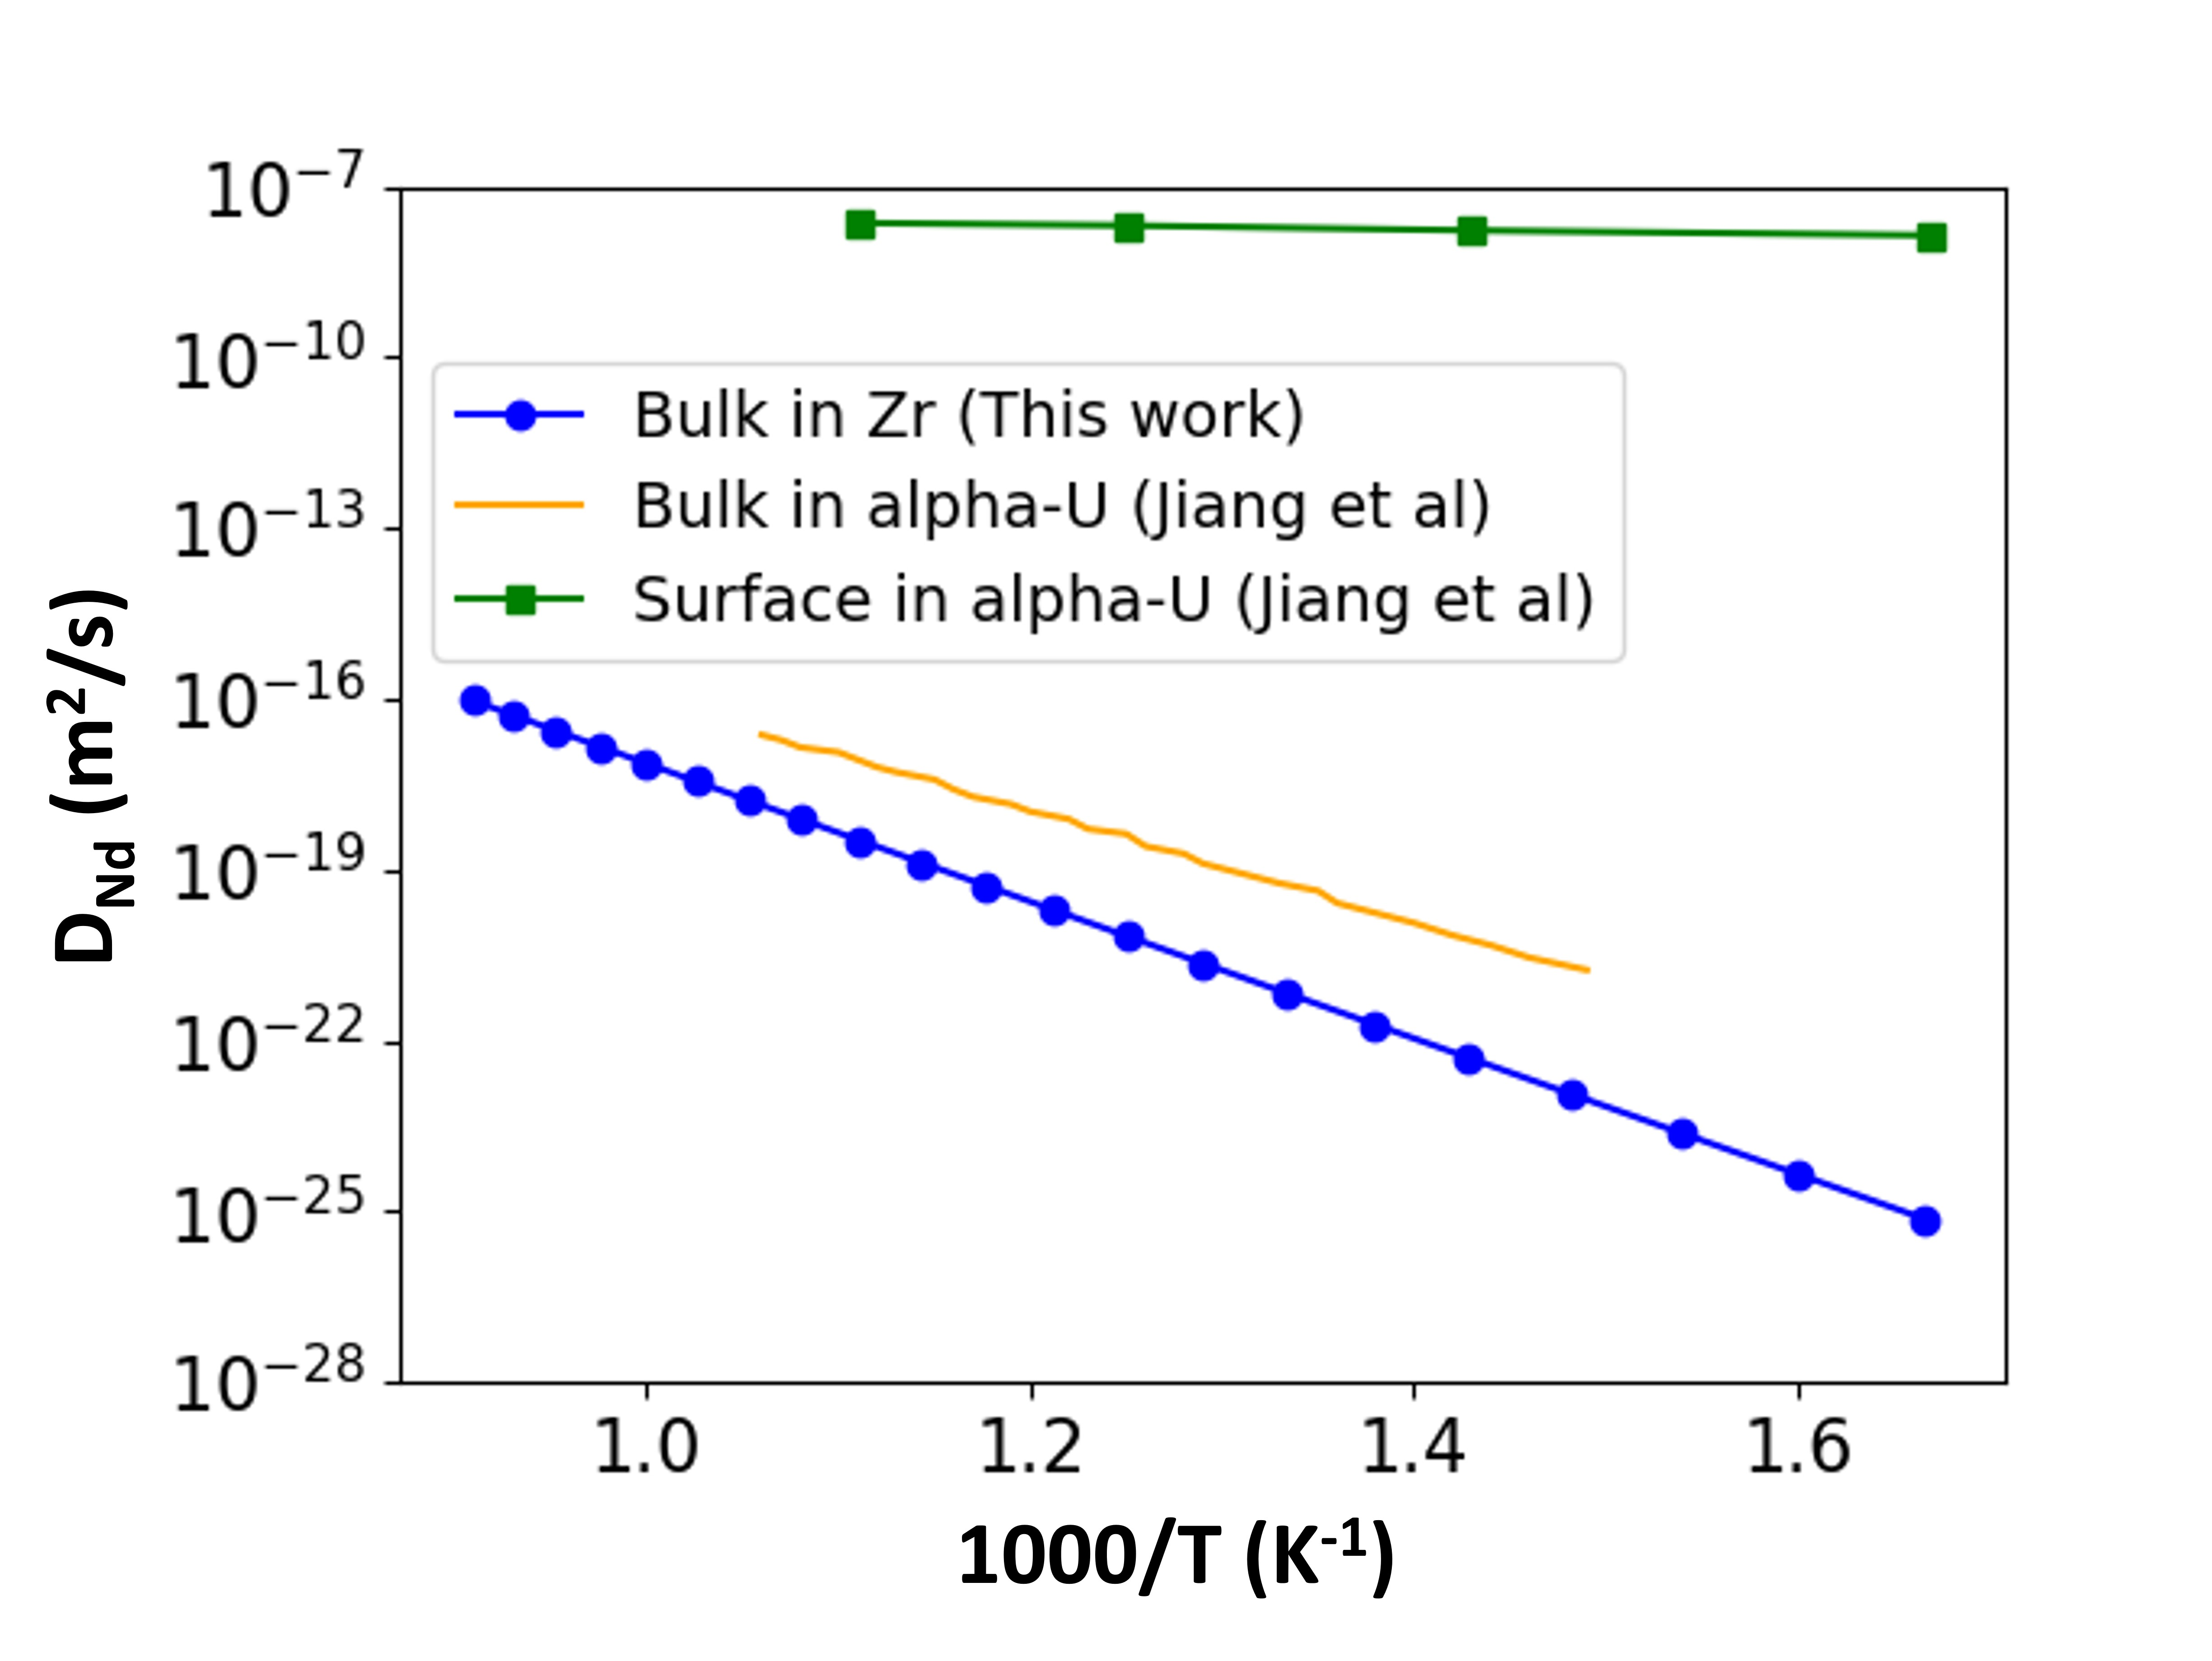
\includegraphics[width=0.8\textwidth]{nd_diff_zr_vs_alphaU_updated.jpg}
%DIFDELCMD <     %%%
\DIFdelendFL \DIFaddbeginFL 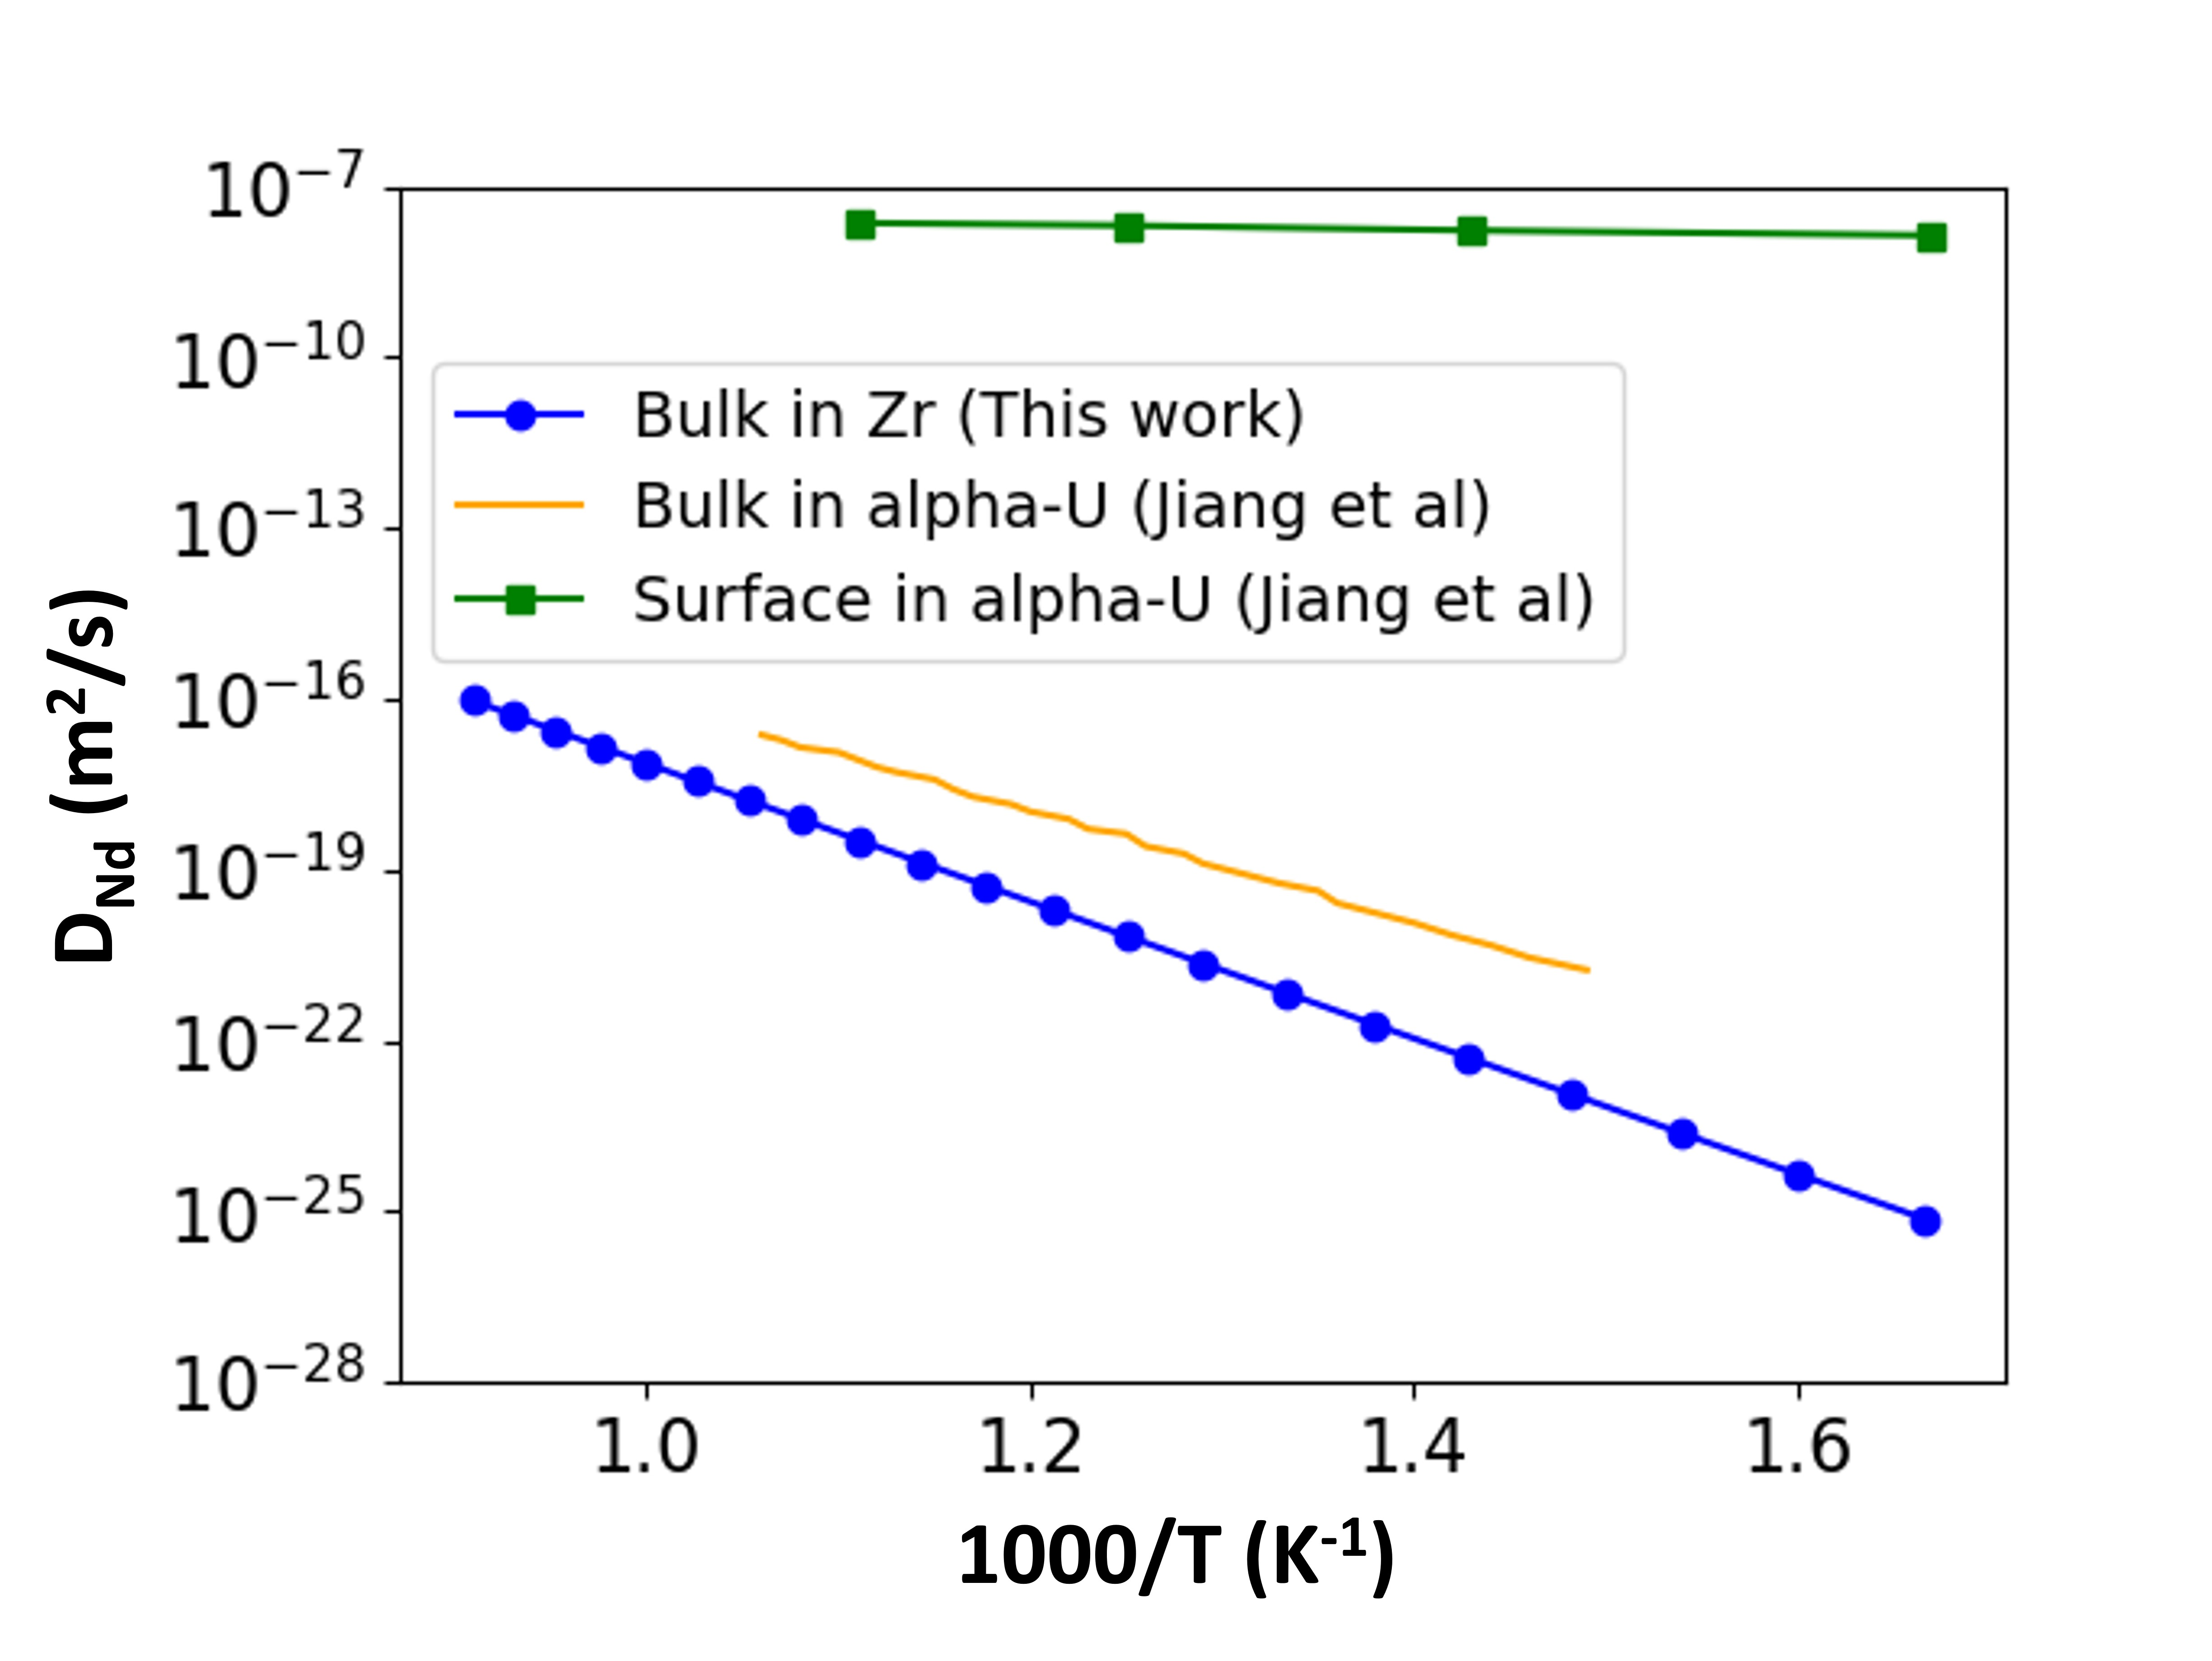
\includegraphics[width=0.7\textwidth]{9_nd_diff_zr_vs_alphaU_updated.jpg}
    \DIFaddendFL \caption{The average (isotropic) bulk diffusivity of Nd in HCP Zr is plotted compared to the bulk and surface diffusivities of Nd in $\alpha$-U from reference \cite{jiang_bulk_2021}}
    \label{fig:nd_av_diff_alphaU}
\end{figure}
\FloatBarrier

The effectiveness of Zr liners as interdiffusion barriers for lanthanides can be also assessed by looking at the segregation tendencies presented in \cref{subsection_drag}. The solute enrichment regimes in \Cref{fig:drag_ratios} \DIFdelbegin \DIFdel{and \Cref{fig:pdc_average} }\DIFdelend indicate that lanthanides will diffuse to vacancy sinks such as grain boundaries and surfaces\DIFaddbegin \DIFadd{, }\DIFaddend and possibly reach the interface of the cladding. The solute depletion regime indicates that lanthanides will diffuse into the bulk Zr and be retained within the Zr matrix. Therefore, the desirable segregation behavior in Zr liners is the depletion tendency at sinks.
Since the enrichment/depletion tendencies of the lanthanides in HCP Zr \DIFdelbegin \DIFdel{is }\DIFdelend \DIFaddbegin \DIFadd{are }\DIFaddend temperature dependent, the optimal case is to ensure that lanthanide depletion takes place at the operating temperature of the liner (T $\approx$ 400 -- 600 \DIFaddbegin \DIFadd{$^{\circ}$}\DIFaddend C) \cite{beausoleil_fast_2022}. Since the temperature of the liner varies along its height and will also depend on the position of the fuel element, the best option is to have a wide temperature range of solute depletion. One way to achieve this is to lower the transition temperature from enrichment to depletion regime. This can be accomplished by controlling the \DIFaddbegin \DIFadd{crystallographic }\DIFaddend grain texture of Zr liners \DIFaddbegin \DIFadd{while maintaining a large grain size to limit grain boundary diffusion}\DIFaddend . According to our results in \Cref{fig:drag_ratios}, solute depletion is dominant for a wider temperature range in the axial direction compared to the basal direction. So, if grain orientations are controlled during manufacturing of the liners to align the c-axis normal to the liner surface, this will provide better retention of lanthanides in the liner. \DIFaddbegin \DIFadd{It should be noted that solute depletion does not mean that lanthanides will never reach the sinks. Solute segregation to grain boundaries due to a thermodynamic preference may still occur. However, controlling the crystallographic orientation of grains will increase the tendency of solutes to remain within the bulk. }\DIFaddend In addition, the effective diffusion coefficient of the lanthanides along the liner thickness will be lower because of the higher activation energy of diffusion in the axial direction than the basal direction as seen in \Cref{fig:diffusivities_ln} and \Cref{tab:arrhenius_fit}.

\section{Conclusion}
For the first time, FCCI-relevant lanthanide (La, Ce, Pr, and Nd) diffusivities in HCP Zr are calculated from the first principles. We employed density functional theory calculations to calculate the formation, binding, and migration energies of vacancies and vacancy-solute pairs. The lanthanide-vacancy pairs have attractive binding energies (0.1 - 0.4 eV) when they are at the $1^{st}$ nearest neighbor position to a vacancy. The binding energies are below 0 (repulsive) at the $2^{nd}$ nearest neighbor and alternate between weak attraction/repulsion beyond that ($|E_b| < $ 0.1 eV). We found that three of the lanthanides (La, Ce, and Pr) behave as oversized solutes. When a lanthanide of these species forms a vacancy-solute pair in a basal plane it occupies an intermediate position between two nearest neighbor lattice sites forming two half vacancies (1b' configuration). This was not observed for non-basal (pyramidal) lanthanide-vacancy pairs \DIFdelbegin \DIFdel{and was not observed }\DIFdelend \DIFaddbegin \DIFadd{or }\DIFaddend in the case of Nd (either basal or non-basal).

The atomistic data was incorporated into the self-consistent mean field theory approach as implemented in the KineCluE code \cite{schuler_kineclue_2020} to calculate the transport coefficients and diffusivities. We found that the four lanthanides have higher diffusivity than Zr self-diffusion by 1-3 orders of magnitude. Our vacancy-mediated diffusion results show that La is the fastest lanthanide and has the least anisotropic behavior with activation energies of 2.26 eV and 2.30 eV in the basal and axial directions, respectively. On the other hand, Pr experiences a large anisotropy with a relatively fast diffusion in the basal plane with an activation energy of 2.29 eV and a slower diffusion along the axial direction with an activation energy of 2.53 eV. Ce and Nd have comparable diffusivities in HCP Zr even though they have different point defect configurations and migration pathways in the HCP lattice (1b' for the Ce-vacancy pair and 1b for the Nd-vacancy pair). The calculated activation energies for Ce are 2.36 eV and 2.45 eV in the basal and axial directions, respectively, while for Nd \DIFdelbegin \DIFdel{, }\DIFdelend they are 2.34 eV and 2.46 eV in the basal and axial directions, respectively. \DIFdelbegin %DIFDELCMD < 

%DIFDELCMD < %%%
\DIFdelend Furthermore, we calculated the vacancy drag ratios and partial diffusion coefficient ratios to extract the depletion/enrichment tendencies of the four lanthanides at vacancy sinks. \DIFdelbegin \DIFdel{According to our results, we expect that in an isotropic polycrystalline Zr, the four lanthanides (La, Ce, Pr, and Nd) are always enriched at sinks at low temperatures and there is a transition to a depletion regime at high temperatures above 875 K . }\DIFdelend We suggest that the transition temperature from enrichment to depletion can be tuned through refining the grain texture. For FCCI liner applications, adjusting grain orientations to align the c-axis perpendicular to the liner surface is desired. This would favor the diffusion of the lanthanides within bulk Zr, resulting in solute depletion at sinks.

Finally, we emphasize that the reported diffusion parameters (activation energies and prefactors) can be a useful input to fuel performance models to quantitatively measure the effectiveness of the Zr liners in limiting the growth of the FCCI region. 

\FloatBarrier
\section{Acknowledgments}

This work was supported by grants from the U.S. Department of Energy, Office of Nuclear Energy (DOE-NE) (DE-NE0009271, Project 22-26632). This research made use of the resources of the High-Performance Computing Center at Idaho National Laboratory, which is supported by the Office of Nuclear Energy of the U.S. Department of Energy and the Nuclear Science User Facilities under Contract No. DE-AC07-05ID14517.

\appendix

\section{Evaluation of Partition Functions and Cluster Fractions}
\label{appendix_partition}

\DIFaddbegin \DIFadd{This appendix is inspired by the formulation presented by Messina et al. \cite{messina_solute_2020} for BCC Fe. }\DIFaddend The total defect concentration includes the concentration of all single vacancies and vacancy-solute pairs:
\begin{equation}
\label{eq_tot_conc}
    C = C_V + C_{VB} - C_{corr}
\end{equation}
where $C_V$ is the concentration of single vacancies and can be obtained at thermodynamic equilibrium from the vacancy formation energy $E_{form}^{vac}$ and vacancy formation entropy $S_{form}^{vac}$ according to the following relation at the dilute limit:
\begin{equation}
\label{eq_vac_conc}
    C_V = Z_V [V] = Z_V e^{\frac{-E_{form}^{vac}}{k_B T}} e^{\frac{S_{form}^{vac}}{k_B}}
\end{equation}
where $Z_V$ is the partition function of isolated single vacancies \DIFaddbegin \DIFadd{per primitive cell }\DIFaddend and corresponds to the number of symmetrically equivalent configurations. For instance, the value of $Z_V$ is 2 for the HCP crystal structure. The second term $C_{VB}$ in \Cref{eq_tot_conc} is the concentration of vacancy-solute pairs and is calculated as follows:
\begin{equation}
    C_{VB} = Z_{VB} [V] [B]
\end{equation}
where $[V]$ is the vacancy concentration in \Cref{eq_vac_conc} and $[B]$ is the solute concentration. \DIFaddbegin \DIFadd{In this work, $[B]$ is assumed fixed to a fixed nominal value ($C_B$) that is used in Equation \ref{solute_diffusion_coeff}. }\DIFaddend $Z_{VB}$ is the pair partition function and is calculated in KineCluE by summation of Boltzmann terms, $exp(\frac{E_{bind}^i}{k_B T})$, for all possible configurations ($i$) for the pair \cite{schuler_kineclue_2020}. Finally, a correction term $C_{corr}$ is subtracted to account for the sites that single vacancies cannot occupy because of the geometrical definition of the vacancy-solute pair. This correction was introduced by Messina et al. \cite{messina_solute_2020} and is defined as:
\begin{equation}
\label{eq_corr_conc}
    C_{corr} = Z_{VB}^0 [V] [B]
\end{equation}
where $Z_{VB}^0$ is the non-interacting cluster partition function and is equal to the number of possible pair configurations within the specified kinetic radius ($r_{kin}$). KineCluE evaluates all the possible jumps up to a maximum trajectory that is equal to $r_{kin}$ and also calculates $Z_{VB}^0$ for that $r_{kin}$. A longer $r_{kin}$ will result in better accuracy. In this work, values of $r_{kin} = 3a, 4a, 5a,$ and $6a$ were explored (where `a' represents the lattice parameter of HCP Zr). We find that a value of $4a$ achieves good convergence and hence was used in all calculations. This resulted in $Z_{VB}^0 = 776$ for the Zr-Nd system and $Z_{VB}^0 = 782$ for the Zr-Ce, Zr-La, and Zr-Pr systems. This difference is due to the presence of different configurations (i.e., the two half vacancies configuration: 1b') for the oversized lanthanides (Ce, La, and Pr). 

The maximum solute concentration $[B]_{max}$ allowed in this dilute model can be derived from the fact that the $C_{corr}$ value cannot exceed the value of $C_V$. By applying this condition using \Cref{eq_vac_conc,eq_corr_conc}:
\begin{equation}
    Z_{VB}^0 [V] [B] < Z_V [V] \Longrightarrow [B] < \frac{Z_V}{Z_{Vb}^0},
\end{equation}
and the maximum solute concentration in the dilute limit for Ce, La, and Pr in HCP Zr is:
\begin{equation}
        [B]_{max} = \frac{2}{782} = 0.256\%
\end{equation}
and for Nd in HCP-Zr is:
\begin{equation}
        [B]_{max} = \frac{2}{776} = 0.258\%
\end{equation}
\DIFaddbegin \DIFadd{It should be noted that all concentrations ($C_V$, $C_{VB}$, $C_{corr}$, and $C_B = [B]$) are given in per-primitive cell quantities. The corresponding per-substitutional site concentrations (i.e., atomic percent) can be easily obtained by multiplying these per-primitive cell concentrations by two. 
}\DIFaddend Finally, the fractions $f_V$ and $f_{VB}$ in \Cref{eq_cluster_exp} can be evaluated by:
\begin{equation}
    f_V = \frac{C_V - C_{corr}}{C}
\end{equation}
\begin{equation}
    f_{VB} = \frac{C_{VB}}{C}.
\end{equation}

\FloatBarrier

\section{Thermodynamic Range Convergence Study}
\label{appendix_conv_th_ra}

\DIFaddbegin \setcounter{figure}{0}

\DIFaddend %Discuss the convergence study of nearest neighbors and thermodynamic threshold (here or in supplementary material)

In this appendix, the convergence of the calculated transport coefficients with the thermodynamic range (ThRa) is presented. The full model used in this work incorporates a ThRa equal to the $6^{th}$ nearest neighbor distance, where all the possible jumps within this range are explicitly calculated using the DFT and CI-NEB methods. This is considered a conservative approach and it required performing CI-NEB calculations for 23 independent jumps for each lanthanide species (listed in \Cref{tab:jumps_vac_oversized} and \Cref{tab:jumps_vac_nd}) in addition to the solute-vacancy exchange jumps in \Cref{tab:jumps}. Since this is computationally expensive, it is worth investigating how reducing this ThRa will impact results.

It is observed in \Cref{fig:convergence_nn} that the results from SCMF calculations using a ThRa of $2^{nd}$ or $3^{rd}$ nearest neighbor distance have large deviations from the full model accounting for all jumps up to the $6^{th}$ nearest neighbor. A ThRa of $4^{th}$ nearest neighbor distance results in more converged behavior and increasing the ThRa to the $5^{th}$ nearest neighbor enhances this convergence and yields almost identical results to that of $6^{th}$ nearest neighbor model.

It should be noted that when decreasing the ThRa, the jumps to the outside of the ThRa are not ignored completely because they are still within the kinetic range. These jumps are treated using the KRA approach \cite{van_der_ven_first_2005}, also known as the linear interpolation of migration barriers (LIMB). This approximation is valid for jumps far away from the solute. However, for jumps in the vicinity of the solute, it may result in large errors. In particular, for solutes in HCP Zr, it was reported by Jain et al.\cite{jain_first-principles_2019} that the LIMB approximation led to overestimating or underestimating the migration barriers by $>$0.1 eV for jumps 1b-4b, 1p-5p, 1b-4$\overline{b}$, and 3c-5p. The deviation of the results using a ThRa of $2^{nd}$ or $3^{rd}$ nearest neighbor distance in \Cref{fig:convergence_nn} agrees with the analysis done by Jain et al. that the LIMB approximation can lead to inaccurate migration barriers for jumps in the vicinity of the solute.

\begin{figure}[h!]
    \centering
    \DIFdelbeginFL %DIFDELCMD < 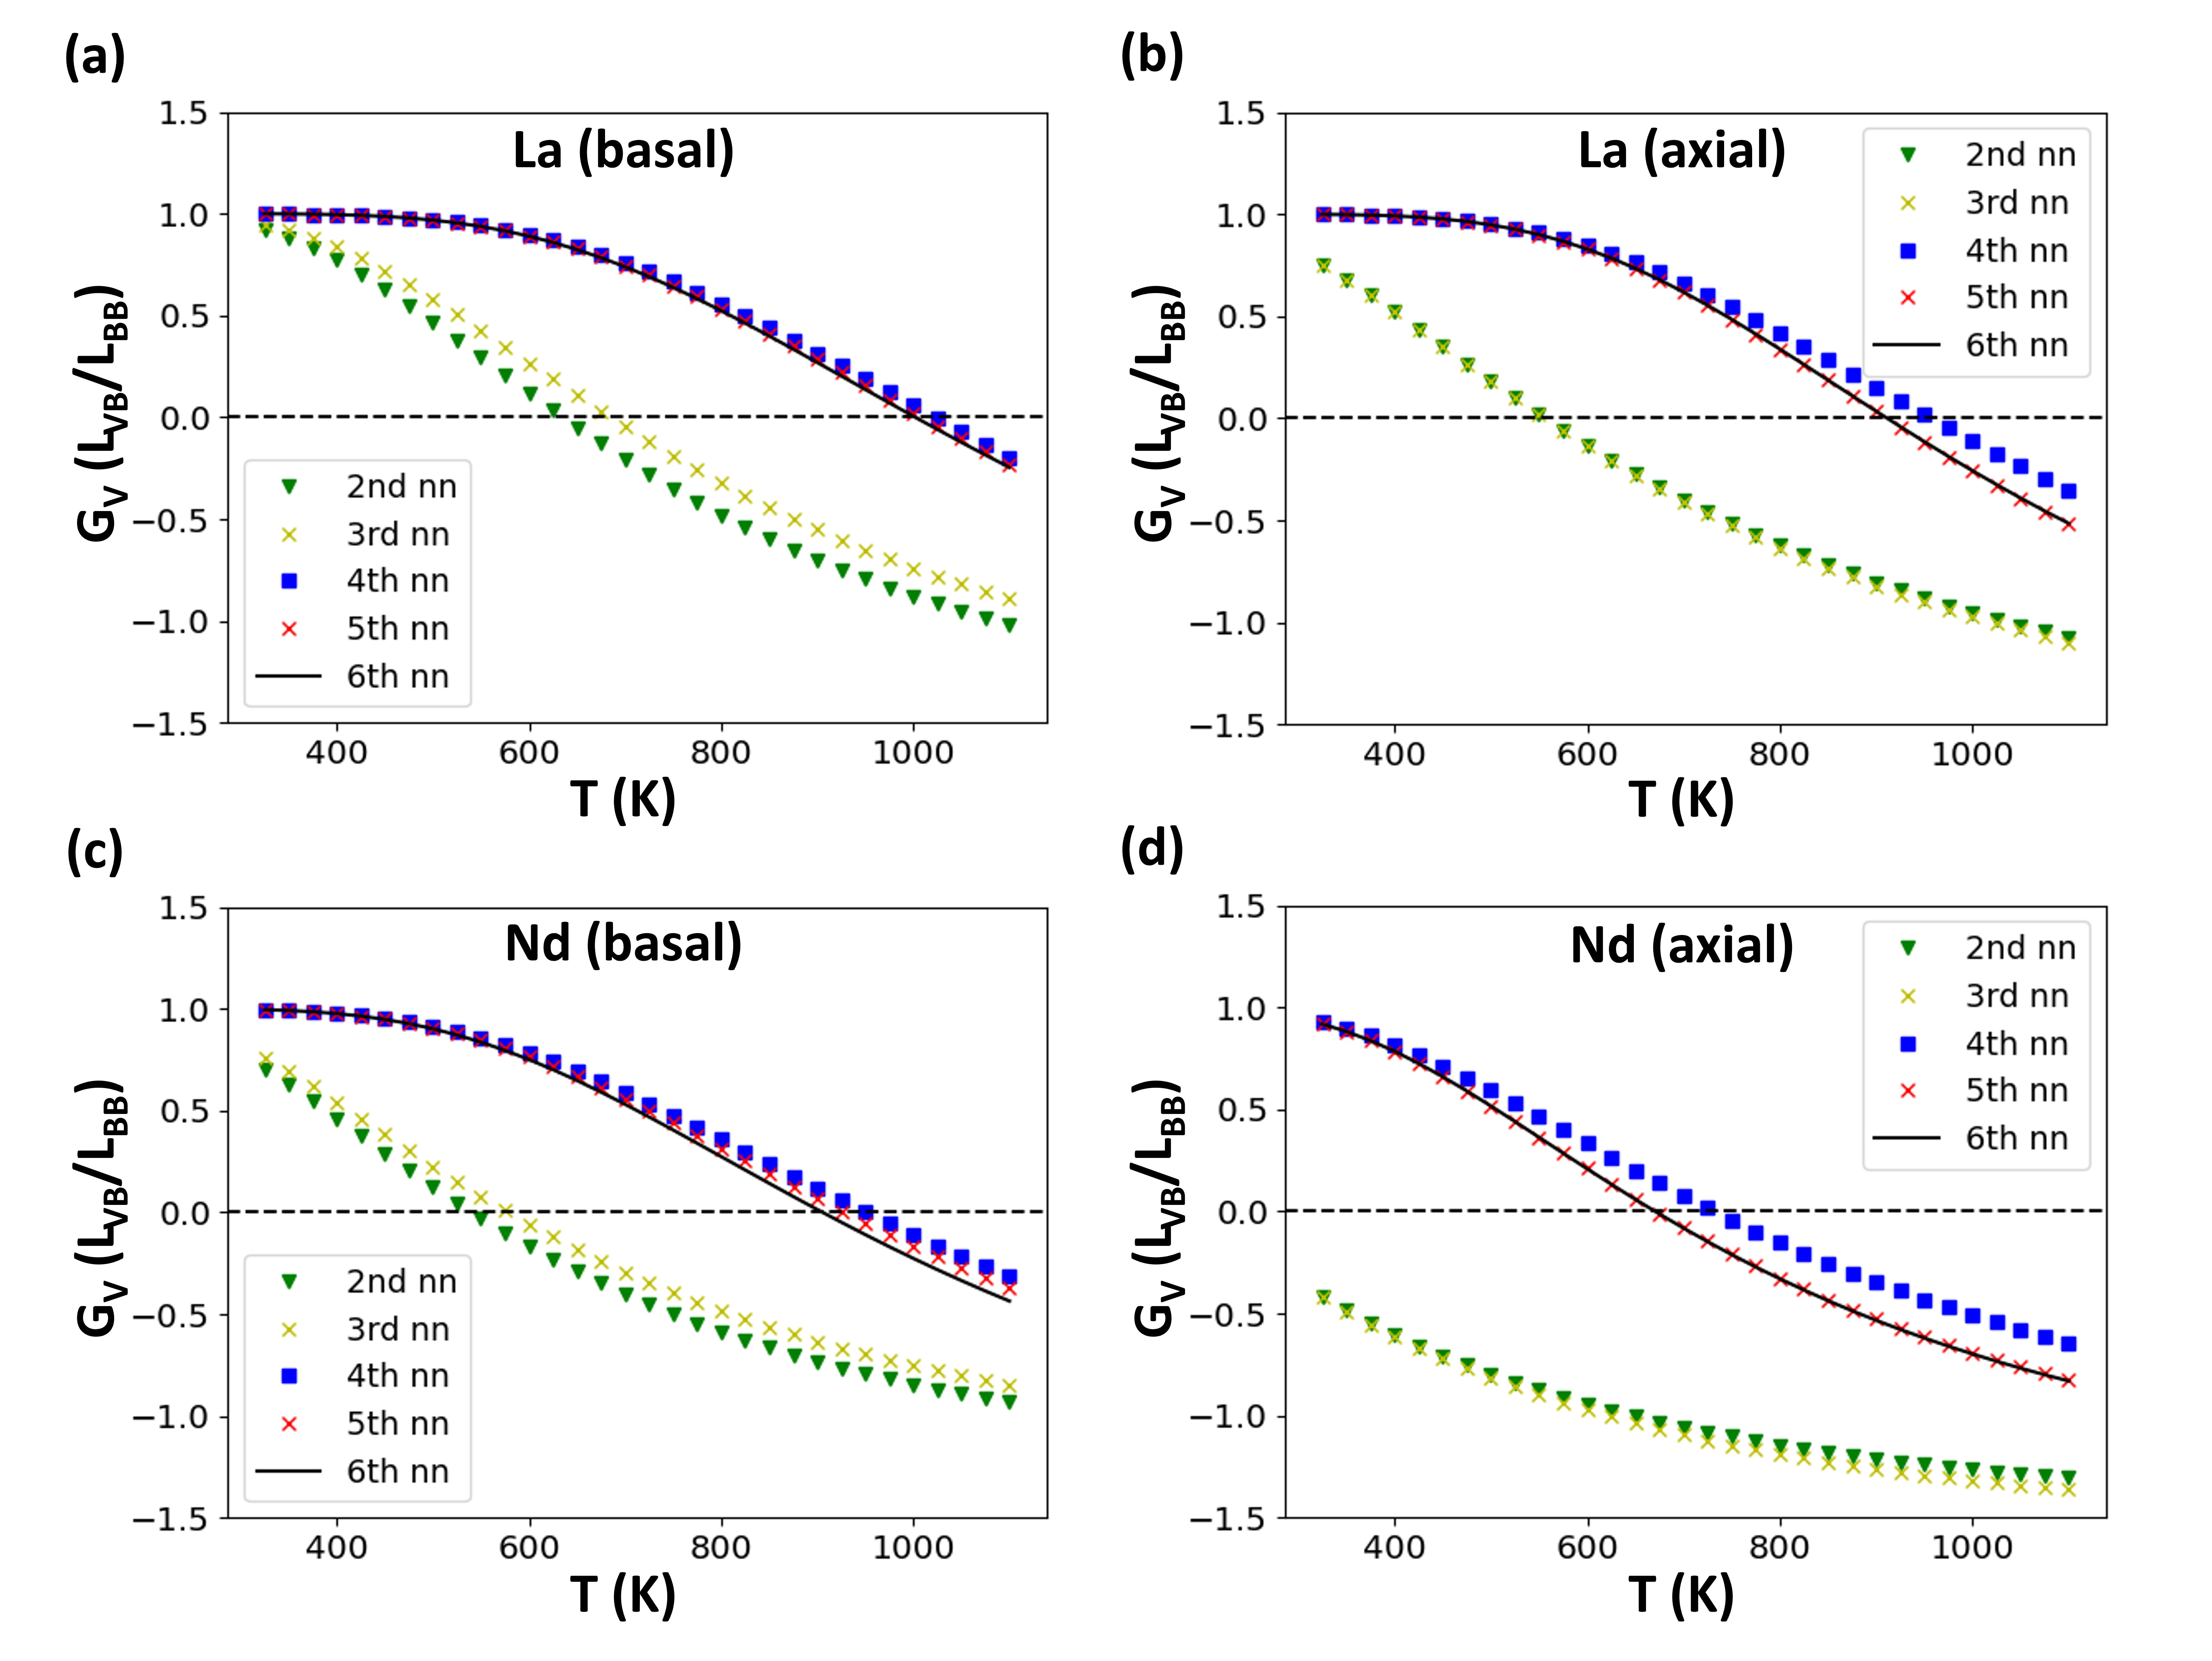
\includegraphics[width=\textwidth]{nn_convergence.jpg}
%DIFDELCMD <     %%%
\DIFdelendFL \DIFaddbeginFL 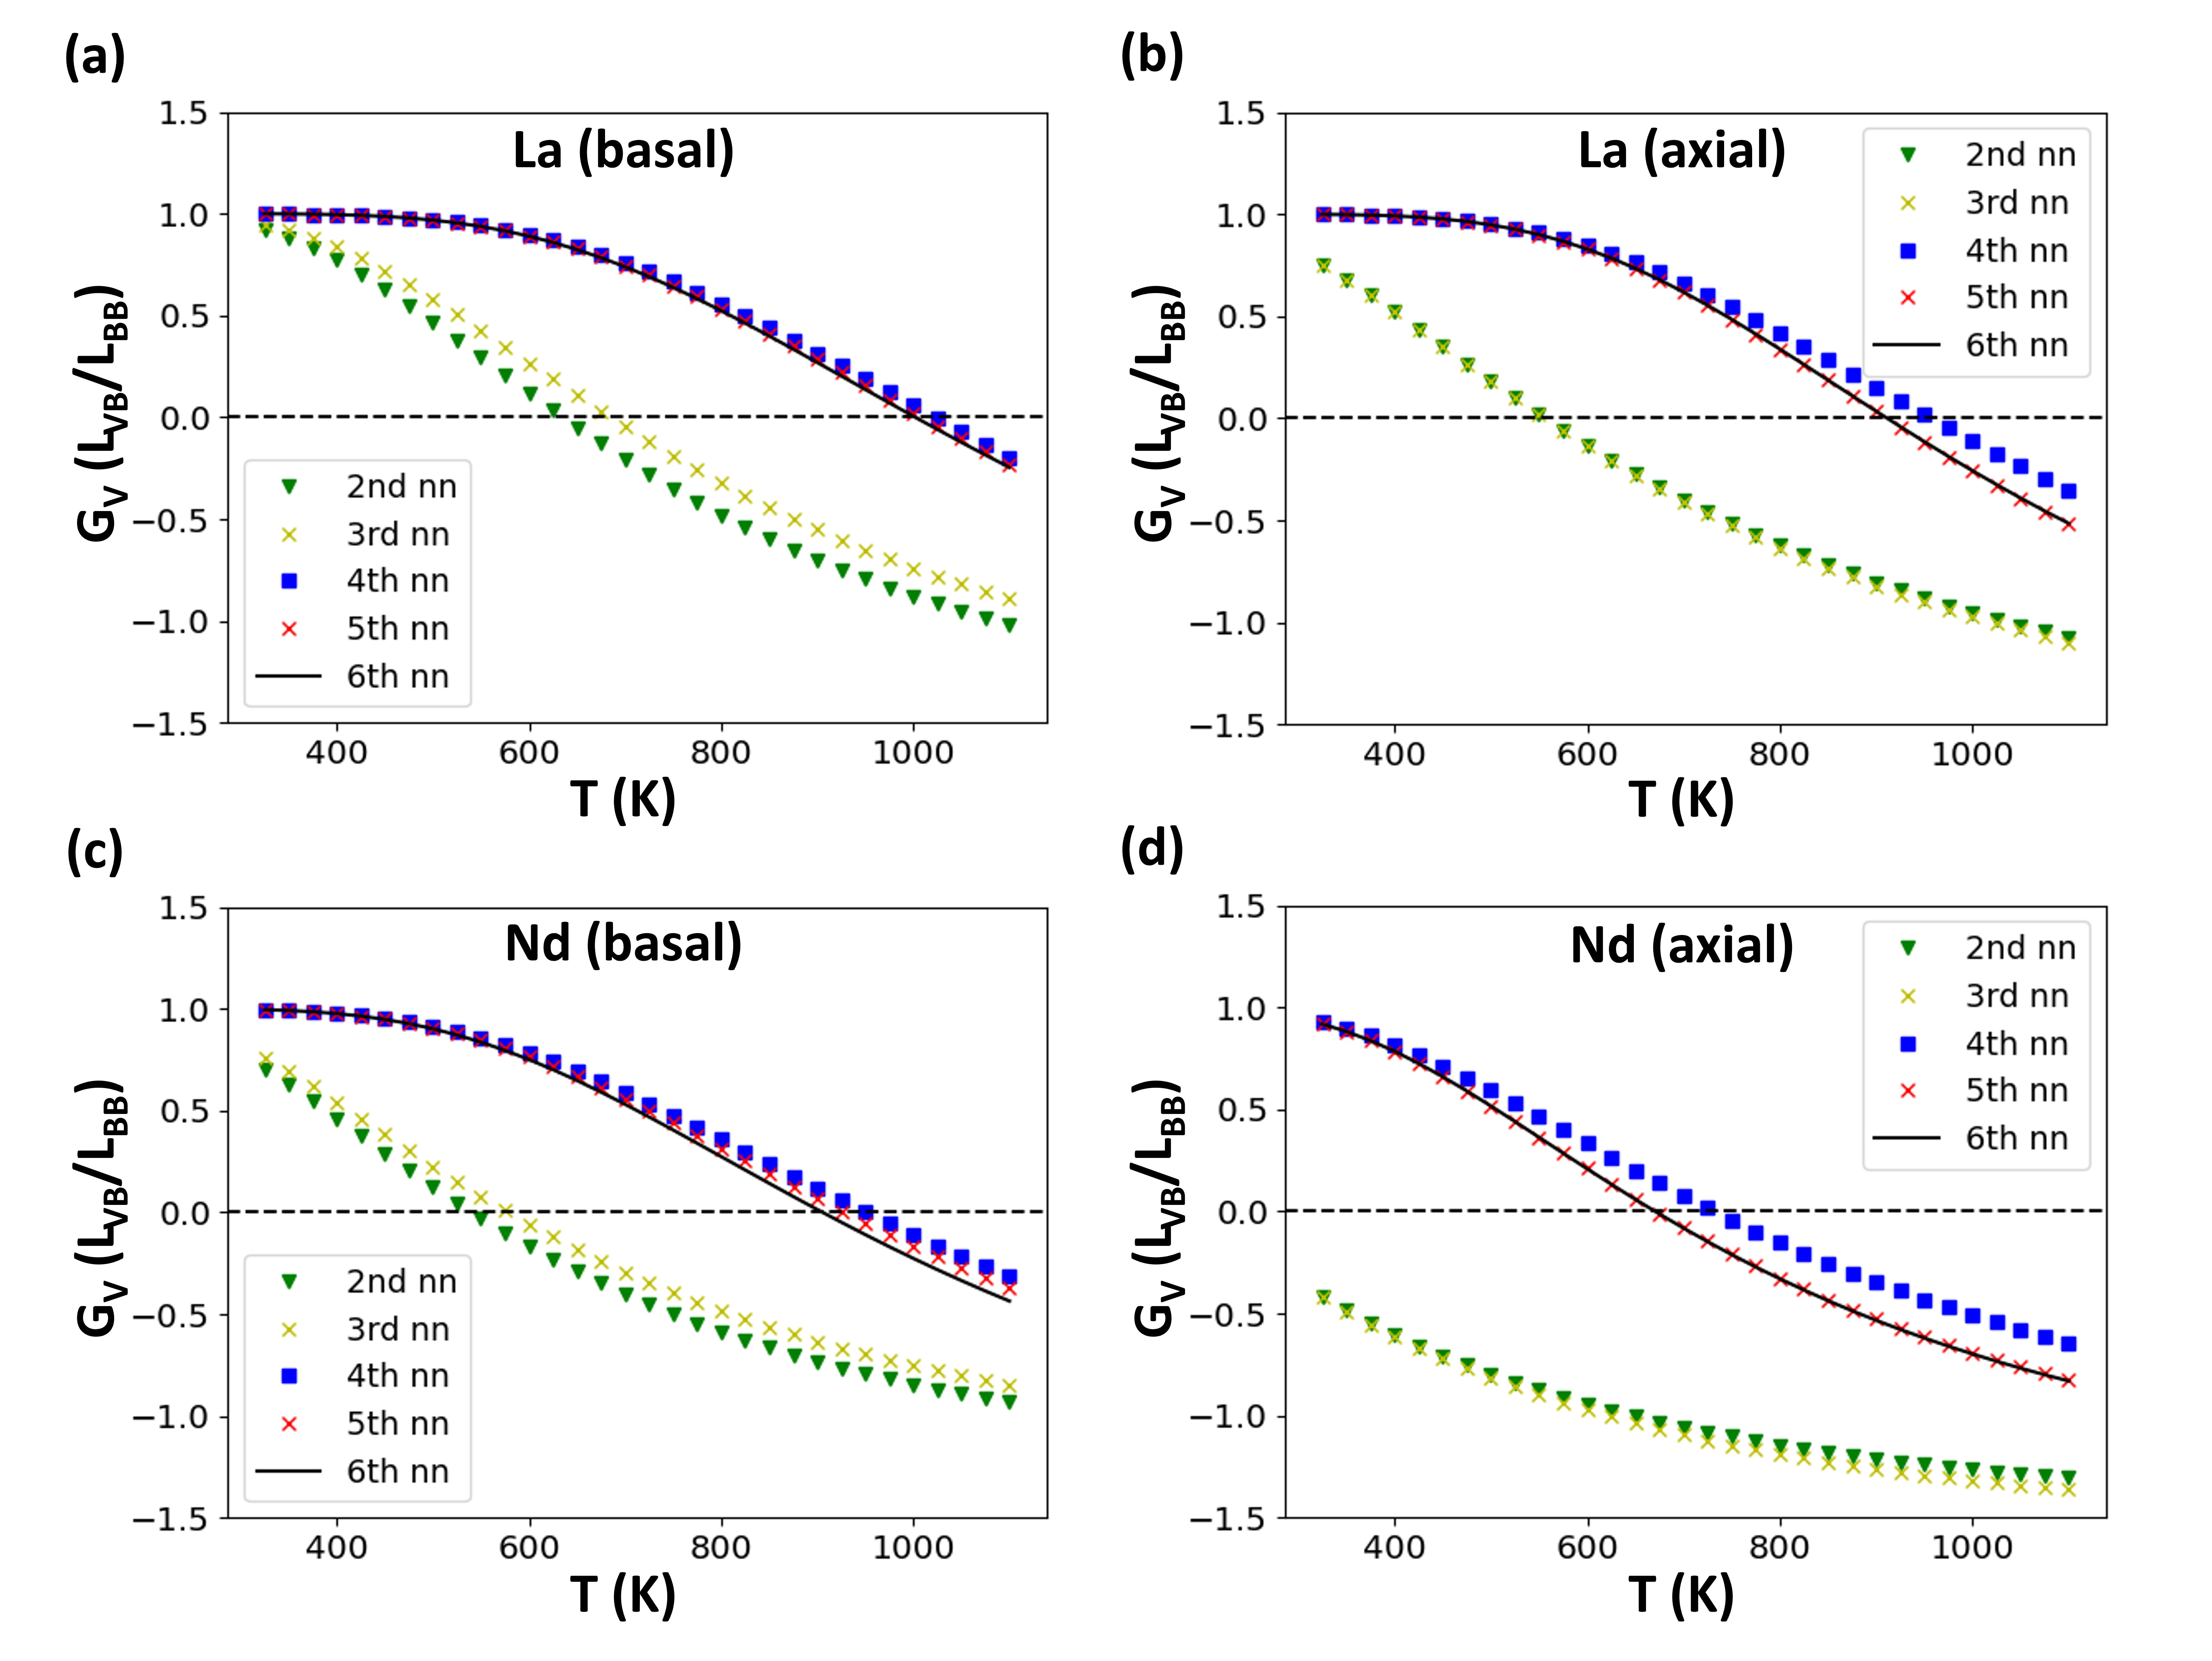
\includegraphics[width=0.9\textwidth]{10_nn_convergence.jpg}
    \DIFaddendFL \caption{Convergence of vacancy drag ratios of La and Nd in HCP Zr with an increase in the thermodynamic threshold (ThRa) from the $2^{nd}$ nearest neighbor to the $6^{th}$ nearest neighbor distance.}
    \label{fig:convergence_nn}
\end{figure}

An alternative approach to calculating all the jumps within the ThRa explicitly is the second shell approximation \cite{nastar_mean_2005, garnier_quantitative_2014}. This approximation is a modified version of the first shell approximation (1nn) where the ThRa value equals the $1^{st}$ nearest neighbor distance. Applying this to the HCP crystal structure yields 5 jumps, basal vacancy-solute exchange, pyramidal vacancy-solute exchange, 1b-1b, 1b-1p, and 1p-1p. In the second shell approximation (1nn)(1nn), other possible jumps from the $1^{st}$ nearest neighbor position are also considered. In the HCP crystal structure, this adds 9 more jumps (1b-2p, 1b-4b, 1b-4$\overline{b}$, 1b-4p, 1b-6b, 1p-2p, 1p-3c, 1p-4p, and 1p-5p). Test results of the first shell (1nn) and second shell (1nn)(1nn) approximation are shown in \Cref{fig:convergence_2nd_shell} compared to the full model with the ThRa = $6^{th}$ nearest neighbor. The vacancy drag ratios from the (1nn)(1nn) agree well with the full model. This indicates that the use of the LIMB approximation for jumps beyond the $1^{st}$ nearest neighbor, even though not very accurate in all cases, has a minimal effect on calculating transport coefficients. In addition, the ability of the (1nn)(1nn) approximation to achieve converged results was also reported in the FCC crystal structure by Garnier et al. \cite{garnier_quantitative_2014}. The convergence study presented in this work suggests that the (1nn)(1nn) approach may be used for solutes in the HCP crystal structures and is computationally more efficient. This approach requires the calculation of 11 fewer migration barriers than those required for the full model (ThRa = $6^{th}$) in the HCP structure.

\begin{figure}[h!]
    \centering
    \DIFdelbeginFL %DIFDELCMD < 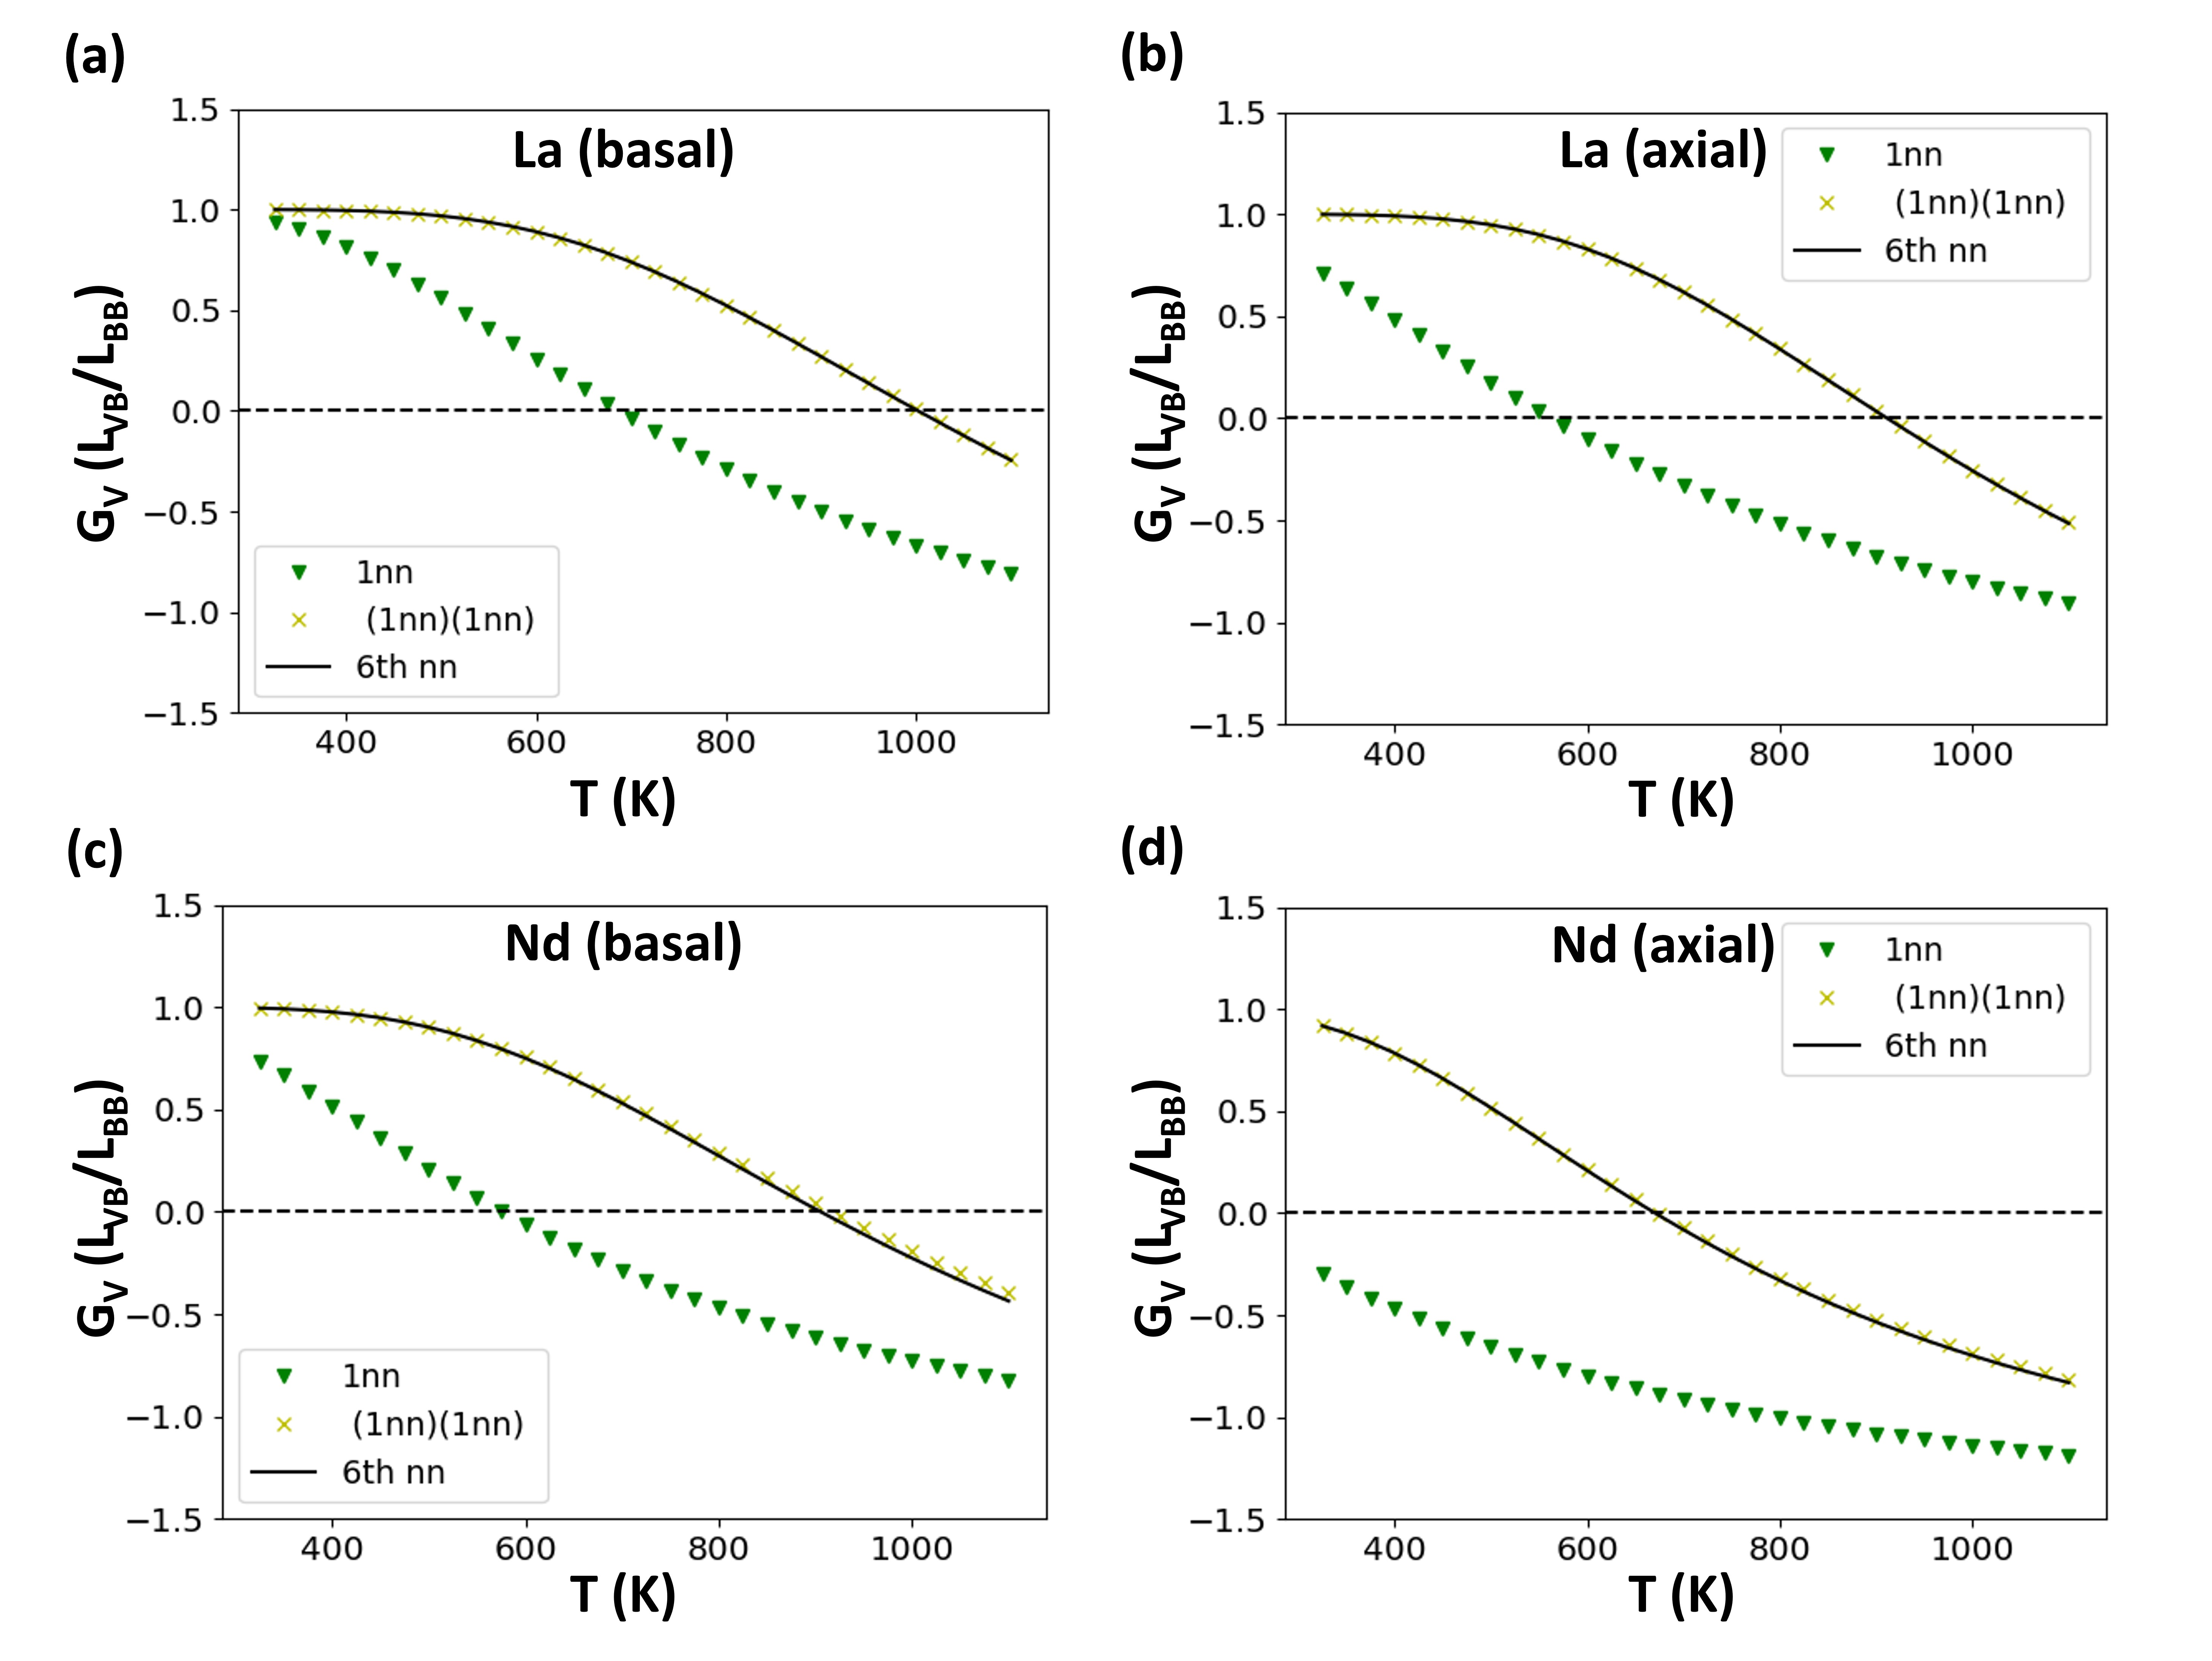
\includegraphics[scale=0.16]{nn_convergence_2nd_shell.jpg}
%DIFDELCMD <     %%%
\DIFdelendFL \DIFaddbeginFL 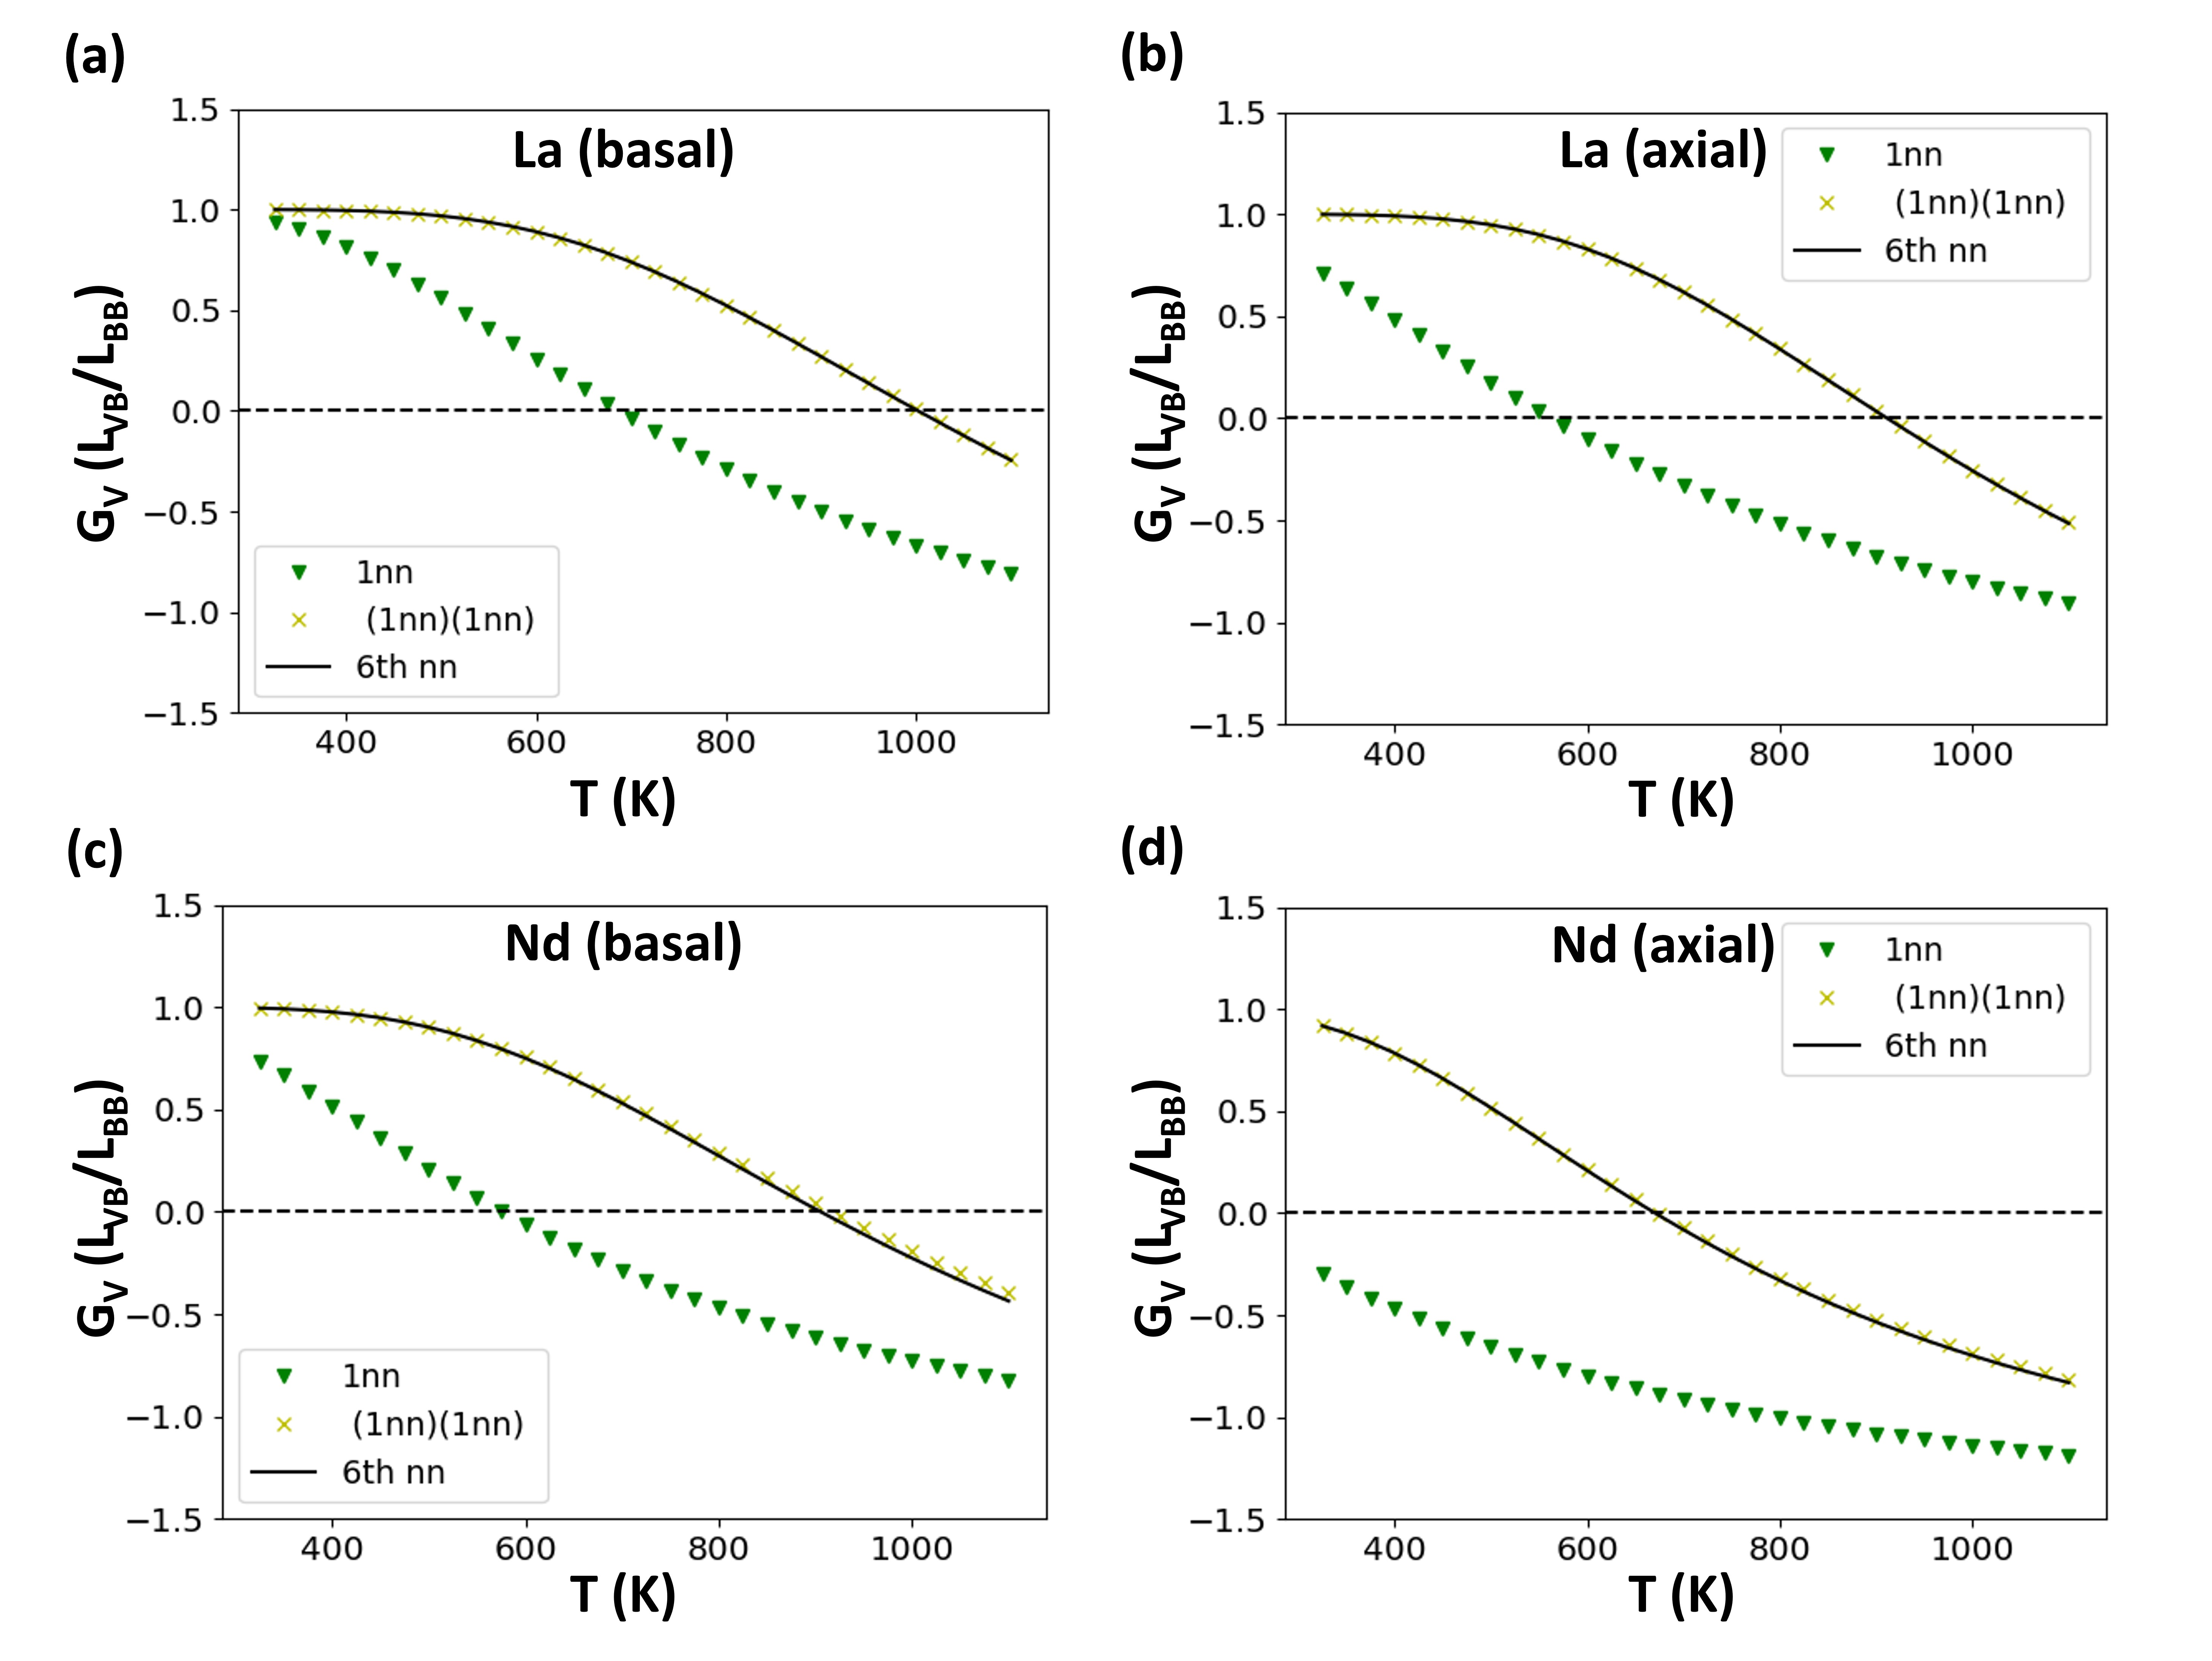
\includegraphics[width=0.9\textwidth]{11_nn_convergence_2nd_shell.jpg}
    \DIFaddendFL \caption{Comparing the vacancy drag ratio results of the first shell approximation (1nn) and the second shell approximation (1nn)(1nn) with the full model (ThRa = $6^{th}$ nn).}
    \label{fig:convergence_2nd_shell}
\end{figure}

\FloatBarrier
\section{DFT data}
\label{app:dft_data}
\DIFaddbegin 

\setcounter{figure}{0}
\setcounter{table}{0}

\DIFaddend The full set of migration barriers and attempt frequencies calculated using DFT for oversized lanthanides in HCP-Zr (La, Ce, and Pr) is reported in \Cref{tab:jumps_vac_oversized} and for Nd in HCP-Zr in \Cref{tab:jumps_vac_nd}.  The migration barriers and attempt frequencies for solute-vacancy exchange jumps are reported earlier in the results section in \Cref{tab:jumps}. 
\DIFdelbegin \DIFdel{The resulting diffusivities of the four lanthanides using all the atomistic data are plotted in \Cref{fig:diffusion_all_lanthanides}.
}\DIFdelend 





\begin{table}[h!]
    \centering
    \caption{The migration barriers ($E_m$) and attempt frequencies ($\nu$) for vacancy jumps in Zr-La, Zr-Ce, and Zr-Pr systems. The notation used for each jump is ``initial configuration"-``final configuration" and the listed migration energies are for the forward jump. The barrier of the backward jump can be deduced from the differences in binding energies between the two configurations.
    $^a$: pyramidal vacancy jump starting from the two half-vacancies configuration (1b') and we assume an attempt frequency equal to that of 1b'-1p jump. $^b$: basal vacancy jump starting from the two half-vacancies configuration (1b') and we assume an attempt frequency equal to that of 1b'-1b'. $^c$ and $^d$: pyramidal and basal vacancy jumps, respectively, where the solute atom remains on the lattice site and we assume an attempt frequency equal to that of the pyramidal and basal monovacancy jumps, respectively. }
    \begin{tabular}{c|c|c|c|c|c|c|c}
    \toprule
       Jump &$E_{m}^{La}$(eV) &$\nu^{La}$(THz) &$E_{m}^{Ce}$(eV) &$\nu^{Ce}$(THz)&$E_{m}^{Pr}$(eV) &$\nu^{Pr}$(THz)  \\
       \hline
       1b'-1b'  &0.788  &1.98 &0.654 &2.83 &0.588 &2.01 \\
       1b'-1p  &1.023  &1.43 &0.820 &2.29 &0.675 &1.53 \\
       1b'-2p  &0.799  &$1.43^{a}$ &0.750 &$2.29^{a}$ &0.709 &$1.53^{a}$ \\
       1b'-4b  &0.597  &$1.98^b$ &0.592 &$2.83^b$ &0.551 &$2.01^b$ \\
       1b'-4$\overline{b}$  &0.473  &$1.98^b$ &0.466 &$2.83^b$ &0.433 &$2.01^b$ \\
       1b'-4p  & 0.640 &$1.43^{a}$ &0.642 & $2.29^{a}$&0.630 &$1.53^{a}$\\
       1b'-6b  &0.644  &$1.98^b$ &0.636 &$2.83^b$ &0.609 &$2.01^b$ \\
       1p-1p  &0.889  &$4.65^d$ &0.515 &$4.65^d$ &0.386 &$4.65^d$ \\
       1p-2p  &0.879  &$4.65^d$ &0.689 &$4.65^d$ &0.638 &$4.65^d$ \\
       1p-3c  &0.772  &$4.58^c$ &0.661 &$4.58^c$ &0.652 &$4.58^c$ \\
       1p-4p  &0.613  &$4.65^d$ &0.507 &$4.65^d$ &0.485 &$4.65^d$ \\
       1p-5p  &0.731  &$4.58^c$ &0.652 &$4.58^c$ &0.628 &$4.58^c$ \\
       2p-4$\overline{b}$  &0.596  &$4.58^c$ &0.599 &$4.58^c$ &0.613 & $4.58^c$\\
       2p-4p  &0.545 &$4.65^d$ &0.555 &$4.65^d$ &0.549 &$4.65^d$ \\
       2p-5p  &0.636  &$4.58^c$ &0.641 &$4.58^c$ &0.647 &$4.58^c$ \\
       3c-5p  &0.556  &$4.65^d$ &0.567 &$4.65^d$ &0.559 &$4.65^d$ \\
       4p-5p  &0.675  &$4.58^c$ &0.664 &$4.58^c$ &0.670 &$4.58^c$ \\
       4p-4p &0.620 &$4.65^d$ &0.616 &$4.65^d$ &0.621 &$4.65^d$ \\
       4b-4p  &0.681  &$4.58^c$ &0.679 &$4.58^c$ &0.694 &$4.58^c$ \\
       5p-5p &0.586 &$4.65^d$ &0.579 &$4.65^d$ &0.576 &$4.65^d$ \\
       6b-4b  &0.589  &$4.65^d$ &0.566 &$4.65^d$ &0.547 &$4.65^d$ \\
       6b-4$\overline{b}$  &0.614  &$4.65^d$ &0.559 &$4.65^d$ &0.543 &$4.65^d$ \\
       6b-4p  &0.654  &$4.58^c$ &0.624 &$4.58^c$ &0.611 &$4.58^c$ \\
       \bottomrule
    \end{tabular}
    \label{tab:jumps_vac_oversized}
\end{table}

\begin{table}[h!]
    \centering
    \caption{The migration barriers and attempt frequencies for vacancy jumps in the Zr-Nd system. The notation used for each jump is ``initial configuration"-``final configuration" and the listed migration energies are for the forward jump. The barrier of the backward jump can be deduced from the differences in binding energies between the two configurations. The superscripts $^c$ and $^d$ are pyramidal and basal vacancy jumps, respectively, where the solute atom remains on the lattice site and we assume an attempt frequency equal to that of the pyramidal and basal monovacancy jumps, respectively.}
    \begin{tabular}{c|c|c}
    \toprule
        Jump&$E_m$ (eV) & $\nu$(THz)  \\
        \hline
       1b-1b &0.705 &$4.65^d$  \\
       1b-1p &0.937 &$4.58^c$ \\
       1b-2p &0.834 & $4.58^c$\\
       1b-4b &0.582 & $4.65^d$\\
       1b-4$\overline{b}$ &0.490 & $4.65^d$\\
       1b-4p &0.662 & $4.58^c$\\
       1b-6b &0.605 & $4.65^d$\\
       1p-1p &0.862 & $4.65^d$\\
       1p-2p &0.798 & $4.65^d$\\
       1p-3c &0.706 & $4.58^c$\\
       1p-4p &0.568 & $4.65^d$\\
       1p-5p &0.689 & $4.58^c$\\ 
       2p-4$\overline{b}$ &0.602 & $4.58^c$\\
       2p-4p &0.546 & $4.65^d$\\
       2p-5p &0.640 & $4.58^c$\\
       3c-5p &0.724 & $4.65^d$\\
       4p-5p &0.675 & $4.58^c$\\
       4p-4p &0.618 & $4.65^d$ \\
       4b-4p &0.675 & $4.58^c$\\
       5p-5p &0.584 & $4.65^d$\\
       6b-4b &0.593 &$4.65^d$ \\
       6b-4$\overline{b}$ &0.623 &$4.65^d$ \\
       6b-4p &0.663 & $4.58^c$\\
       \bottomrule
    \end{tabular}
    \label{tab:jumps_vac_nd}
\end{table}

\FloatBarrier

\DIFdelbegin %DIFDELCMD < \begin{figure}
%DIFDELCMD <     %%%
\DIFdelendFL \DIFaddbeginFL \section{\DIFaddFL{Correlation Factors}}
\label{appendix_correlation}

\setcounter{figure}{0}
\setcounter{table}{0}

\DIFaddFL{The correlation factors ($F_{ij}$) measure the deviation from the random-walk behavior in the transport of atoms. $F_{ij}$s of solute and self-diffusion can be extracted from the KineCluE output \cite{schuler_kineclue_2020}. It is calculated from the ratio of a transport coefficient to its uncorrelated contribution \cite{schuler_kineclue_2020} as follows:
}

\begin{equation}
    \DIFaddFL{F_{ij} = \frac{L_{ij}}{L_{ij}^0}
}\end{equation}

\DIFaddFL{The diffusion coefficients of lanthanides in HCP Zr 
and the corresponding correlation factors are plotted versus inverse temperature in Figure \ref{fig:correlation_factors}. In principle, the correlation factors depend also on solute concentration. However, in the dilute-limit model used in this work, the correlation factors and diffusion coefficients are independent of concentration.
}

\begin{figure}[h!]
    \DIFaddendFL \centering
    \DIFdelbeginFL %DIFDELCMD < 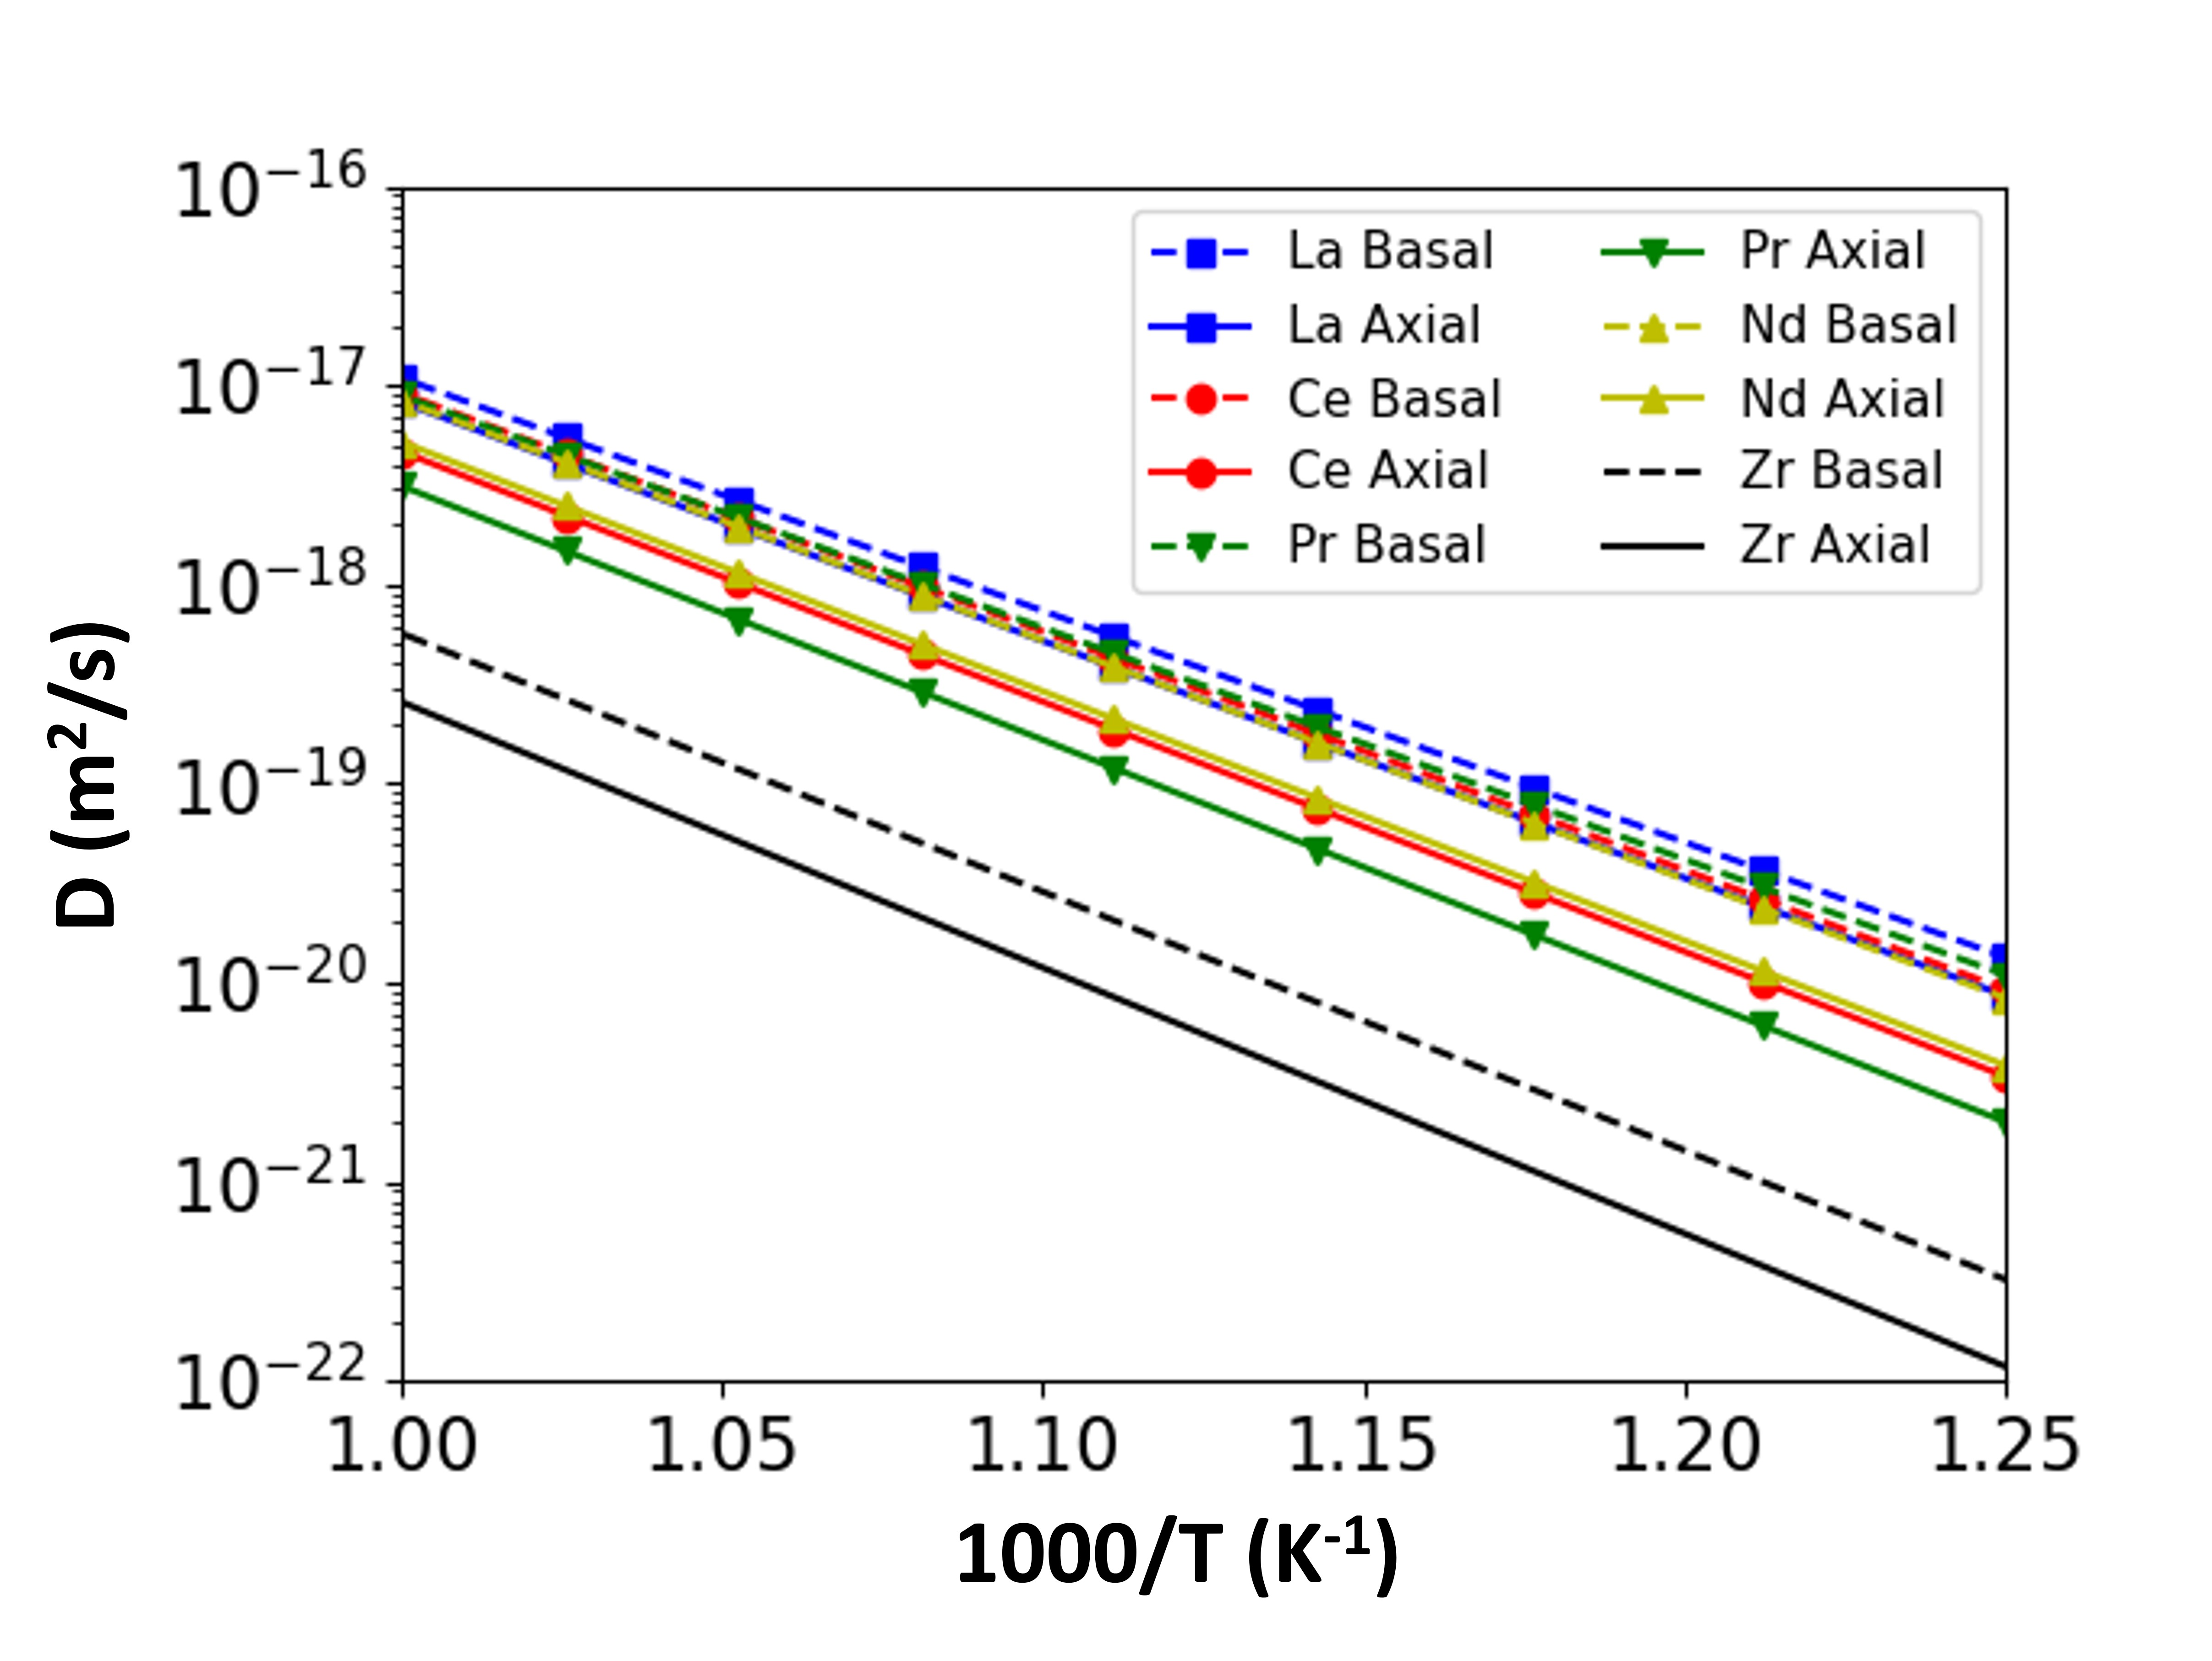
\includegraphics[scale=0.2]{diff_all.jpg}
%DIFDELCMD <     %%%
\DIFdelendFL \DIFaddbeginFL 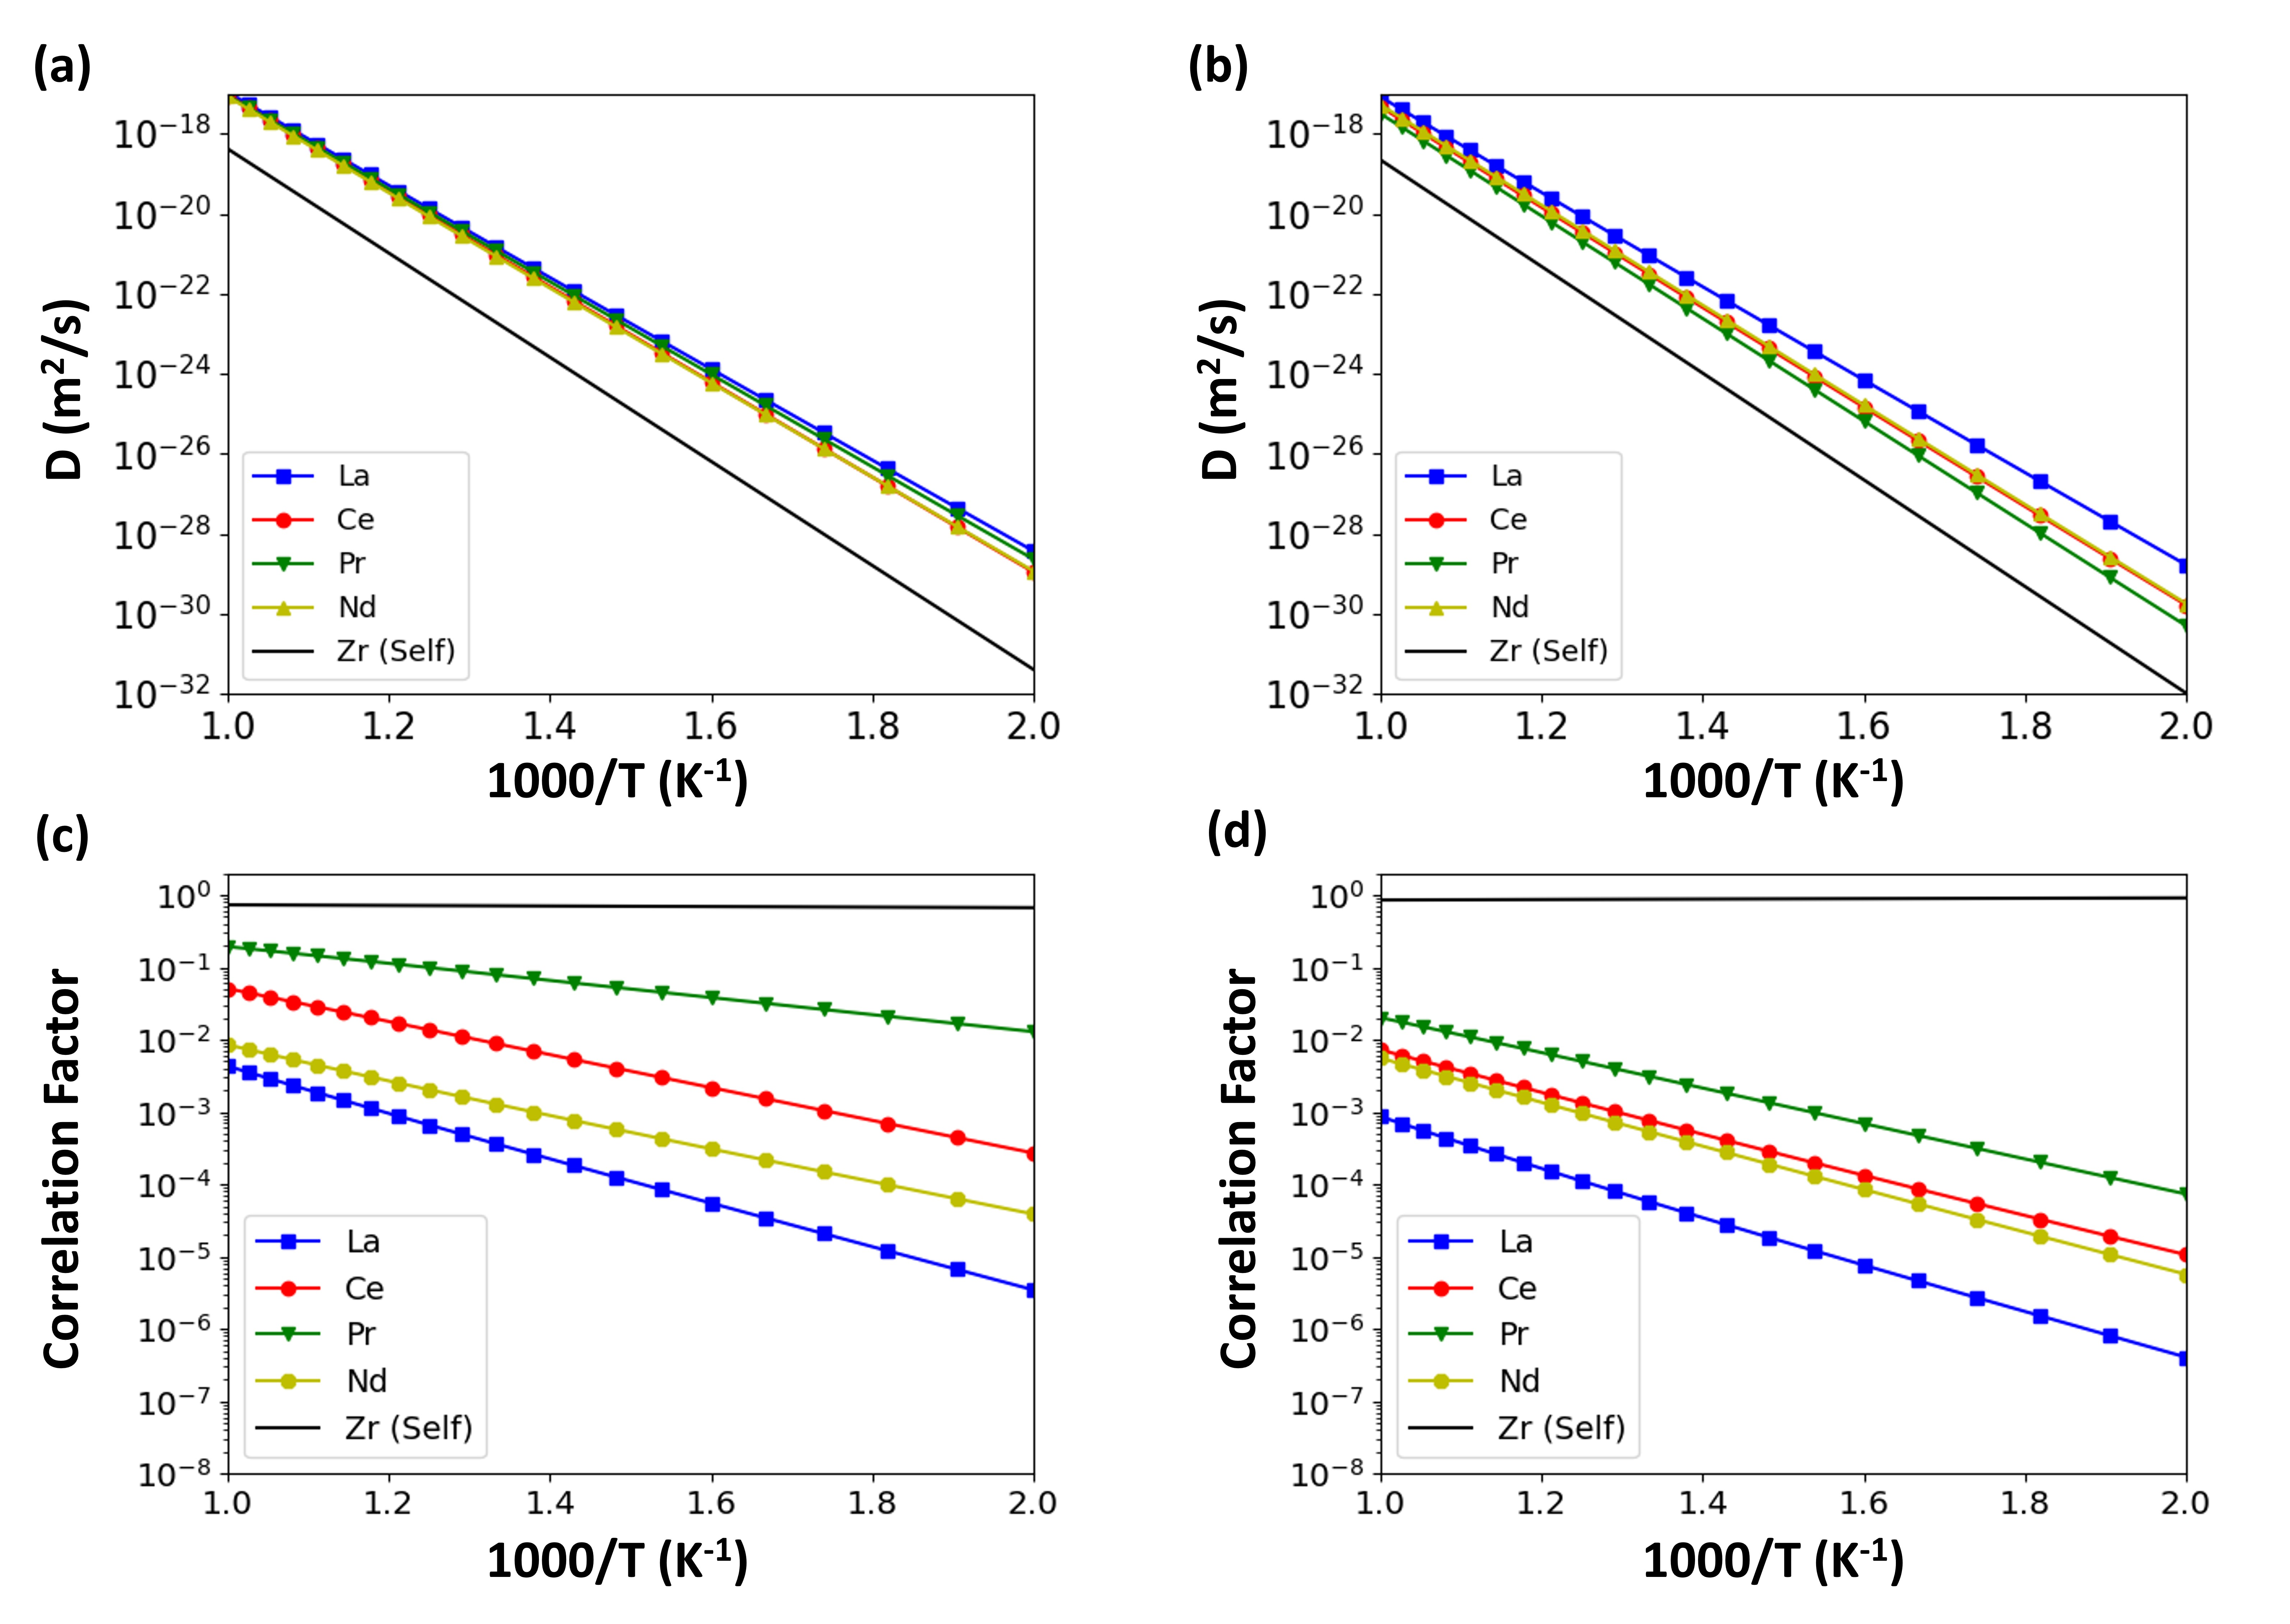
\includegraphics[width=0.9\textwidth]{13_correlation_factors.jpg}
    \DIFaddendFL \caption{The \DIFdelbeginFL \DIFdelFL{diffusivity }\DIFdelendFL \DIFaddbeginFL \DIFaddFL{diffusion coefficients }\DIFaddendFL of La, Ce, Pr, and Nd in \DIFdelbeginFL \DIFdelFL{both basal }\DIFdelendFL (\DIFdelbeginFL \DIFdelFL{dashed lines}\DIFdelendFL \DIFaddbeginFL \DIFaddFL{a}\DIFaddendFL ) \DIFaddbeginFL \DIFaddFL{basal, }\DIFaddendFL and \DIFdelbeginFL \DIFdelFL{axial }\DIFdelendFL (\DIFdelbeginFL \DIFdelFL{solid lines}\DIFdelendFL \DIFaddbeginFL \DIFaddFL{b}\DIFaddendFL ) \DIFaddbeginFL \DIFaddFL{axial }\DIFaddendFL directions are plotted versus inverse temperature between T = \DIFdelbeginFL \DIFdelFL{800 }\DIFdelendFL \DIFaddbeginFL \DIFaddFL{500 }\DIFaddendFL K and T = 1000 K. The \DIFdelbeginFL \DIFdelFL{self-diffusivity of Zr is }\DIFdelendFL \DIFaddbeginFL \DIFaddFL{corresponding correlation factors are }\DIFaddendFL plotted in \DIFaddbeginFL \DIFaddFL{(c) and (d) for basal and axial directions, respectively. Self-diffusion coefficients and the corresponding correlation factors are plotted in solid }\DIFaddendFL black \DIFaddbeginFL \DIFaddFL{lines}\DIFaddendFL .}
    \DIFdelbeginFL %DIFDELCMD < \label{fig:diffusion_all_lanthanides}
%DIFDELCMD < %%%
\DIFdelendFL \DIFaddbeginFL \label{fig:correlation_factors}
\DIFaddendFL \end{figure}

\FloatBarrier
 \DIFdelbegin %DIFDELCMD < 

%DIFDELCMD <  %%%
\DIFdelend \bibliographystyle{elsarticle-num} 
\bibliography{references_file}



\end{document}
